 %%%%%%%%%%%%%%%%%%%% book.tex %%%%%%%%%%%%%%%%%%%%%%%%%%%%%
%
% sample root file for the chapters of your "monograph"
%
% Use this file as a template for your own input.
%
%%%%%%%%%%%%%%%% Springer-Verlag %%%%%%%%%%%%%%%%%%%%%%%%%%


% RECOMMENDED %%%%%%%%%%%%%%%%%%%%%%%%%%%%%%%%%%%%%%%%%%%%%%%%%%%
%\documentclass{class/svmonoGV_large}
\documentclass{class/svmono}
\usepackage[dutch, english]{babel}
% choose options for [] as required from the list
% in the Reference Guide, Sect. 2.2

\usepackage{makeidx}         % allows index generation
\usepackage[pdftex]{graphicx}        % standard LaTeX graphics tool
% when including figure files
\usepackage{multicol}        % used for the two-column index
\usepackage[bottom]{footmisc}% places footnotes at page bottom
%\newcommand{\vet}[1]{{\ensuremath{\mbox{\boldmath $#1$}}}}
%\newtheorem{definition}{Definition}
%\newtheorem{theorem}{Theorem}
%\newtheorem{example}{Example}
\usepackage{hyperref}
\usepackage{amsmath}
\usepackage{multirow}
\usepackage{color}
\usepackage{subfigure}
\usepackage{natbib}
\usepackage{amsfonts}
\usepackage{amssymb}
\usepackage{epsfig}
\usepackage{makeidx}
\usepackage{pdfpages}
\usepackage{rotating}
\usepackage{listings}
\usepackage[left=2cm, right=2cm, top=2.7cm, bottom=2.7cm,]{geometry} 
%\usepackage{apacite}

\lstset{language=R,
	basicstyle=\small\ttfamily,
	stringstyle=\color{DarkGreen},
	otherkeywords={0,1,2,3,4,5,6,7,8,9},
	morekeywords={TRUE,FALSE},
	deletekeywords={data,frame,length,as,character},
	keywordstyle=\color{blue},
	commentstyle=\color{DarkGreen},
}
% etc.
% see the list of further useful packages
% in the Reference Guide, Sects. 2.3, 3.1-3.3
\geometry{paperwidth=17cm, paperheight=24cm}
% \usepackage[
%   noinfo,
%   cam,
%   cross,                % crosses as marks
%   width=17.6cm,         % the width of the galley
%   height=24.6cm,        % the height of the galley
%   center                % actual page is centered on the galley
% ]{crop}    
\makeindex             % used for the subject index
% please use the style svind.ist with
% your makeindex program


%%%%%%%%%%%%%%%%%%%%%%%%%%%%%%%%%%%%%%%%%%%%%%%%%%%%%%%%%%%%%%%%%%%%%

\begin{document}
	%
	%\author{Author(s)}
	%\title{Insert your Booktitle, Subtitle, Edition\\
	%{\small SPIN Springer's internal project number, if known}}
	%\subtitle{-- Monograph --}
	%\maketitle
	
	%for cosmetic reasons I include the front cover
	% REMOVE THE BELOW LINE WHEN SENDING TO PRINTER
	%\includepdf{cover_front.pdf}
	
	\titlepage{
		
		\author{Mingyang Cai\\ Utrecht University, Utrecht}
		\title{Informed Strategies for Multivariate Missing Data}
		\maketitle
		
		%	\newpage
		%	\thispagestyle{empty}
		%	\mbox{}
		
		\newpage
		\thispagestyle{empty}
		\begin{center}
			
			{\Huge Informed Strategies for }\\ \vspace{0.25cm}
			{\Huge Multivariate Missing Data}
			
			\vspace{2 cm}
			
			Geïnformeerde strategieën voor ontbrekende multivariate gegevens
			
			(met een samenvatting in het Nederlands)
			
			\vspace{3cm}
			
			\textbf{Proefschrift}         \\
			
			
			\vspace{3cm}
			
			ter verkrijging van de graad van doctor aan de \\
			Universiteit Utrecht\\
			op gezag van de\\
			rector magnificus, prof.dr. H.R.B.M. Kummeling,\\
			ingevolge het besluit van het college voor promoties\\ 
			in het openbaar te verdedigen op\\
			
			vrijdag 7 oktober 2022 des middags te 12.15 uur 
			
			\vspace{2cm}
			
			door           \\
			
			\vspace{.5cm}
			
			\textbf{Mingyang Cai}      \\
			
			\vspace{.5cm}
			
			geboren op 31 oktober 1992 \\
			te Jiangsu, China
		\end{center}
		
		\newpage
		\thispagestyle{empty}
		\begin{tabular}{lll}
			\textbf{Promotor:}    & & Prof.dr. S. van Buuren \\
			\textbf{Copromotor:} &  &   Dr. G. Vink \\      
		\end{tabular}
		\vspace{\fill}
		
		
		%\noindent Vink, Gerrit \\
		%Restrictive Imputation of Incomplete Survey Data \\
		%Proefschrift Universiteit Utrecht, Utrecht. - Met lit. opg. - Met samenvatting in het Nederlands. \\
		%ISBN: ISBN NR \\
		%Druk: DRUKKER INFO \\
		%Cover designed by Gerko Vink \\
		%Copyright $\copyright$ 2014, G. Vink. All Rights Reserved.\\
		%
		%
		%{\tiny
		%\noindent Neither this book nor any part may be reproduced or transmitted in any form or by any means, electronic or mechanical,
		%including photocopying, microfilming, and recording, or by any information storage and retrieval system, without written
		%permission of the author.
		%Alle rechten voorbehouden. Niets uit deze uitgave mag worden verveelvuldigd, in enige vorm of op enige wijze,
		%zonder voorafgaande schriftelijke toestemming van de auteur.
		%}
		\newpage
		\thispagestyle{empty}
		%\begin{tabular}{lll}
		\noindent \textbf{Beoordelingscommissie:} \\
		
		\noindent Prof. dr. A.G. de Waal\\
		Prof. dr. D. Rizopoulos\\
		Prof. dr. D.L. Oberski\\
		Prof. dr. J. Vermunt\\
		Dr. S. Jolani\\
		
		
		%\end{tabular}
		\vspace{\fill}
		
		
		%\noindent Vink, Gerko \\
		%Restrictive Imputation of Incomplete Survey Data \\
		%Proefschrift Universiteit Utrecht, Utrecht. - Met lit. opg. - Met samenvatting in het Nederlands. \\
		%ISBN 978-90-393-6300-3 \\
		%Druk: GVO drukkers \& vormgevers B.V. $|$ Ponsen \& Looijen \\
		%Cover design by Gerko Vink \\
		%Copyright $\copyright$ 2015, G. Vink. All Rights Reserved.\\
		
		{\small \noindent 
		}
		
		%\newpage
		%\thispagestyle{empty}
		%\mbox{}
		
		
		
		
		\frontmatter%%%%%%%%%%%%%%%%%%%%%%%%%%%%%%%%%%%%%%%%%%%%%%%%%%%%%%
		
		%%%%%%%%%%%%%%%%%%%%%% pref.tex %%%%%%%%%%%%%%%%%%%%%%%%%%%%%%%%%%%%%
%
% sample preface
%
% Use this file as a template for your own input.
%
%%%%%%%%%%%%%%%%%%%%%%%% Springer-Verlag %%%%%%%%%%%%%%%%%%%%%%%%%%

\Preface

%% Please write your preface here
I wish to express my gratitude to the people who have been instrumental in completing this project. I would like to show my greatest appreciation to my supervisors. Stef, I thank you for your valuable guidance and advice. Without your vast knowledge of statistics, this project would not have been possible. You inspired me greatly to research multiple imputations and has been critical to my scientific growth. Deep gratitude is also due to Gerko, my daily supervisor. Two meetings every week, parties held at your home and tips for living in the Netherlands, all these things make me feel at home away from home. I learn a lot from your elegant programming. I still remember your words at our first meeting: the PhD project is to prove your ability to conduct research independently. This word really leads the way to my project. I was pleased to have supervision from both of you.

I thank everyone once joined in the weekly mice meeting. The shared works and ideas, the discussed questions during the meeting really have an influence on me. Furthermore, I am grateful to everyone from M\&S at Utrecht University. I enjoyed various kinds of research meetings and activities here. 

My friends and family are important to me. I thank my parents for giving me the opportunity to learn more about statistics and develop skills to conduct scientific research. You could not have given me a greater gift. I also thank my brother and friends to make a joyful life.

%% Please "sign" your preface
\vspace{1cm}

\begin{flushright}\noindent
Utrecht, October 2022\\
{\it Mingyang Cai}
\end{flushright}

		\tableofcontents
		
		
		\mainmatter%%%%%%%%%%%%%%%%%%%%%%%%%%%%%%%%%%%%%%%%%%%%%%%%%%%%%%%
		\chapter{Introduction} 
\label{chap1}
	Missing data commonly occur in scientific research and have a significant impact on the downstream analysis. First, most statistical analyses require complete data and can not apply to incomplete data directly. Second, the reduced sample size arose from missing data generally induces estimates with less efficiency and results with a loss of statistical power \citep{RubinD1987}.

For instance, in clinical research, investigators may encounter difficulties of prognostic covariates measurement, such as estrogen receptor status, nodal status, or size of the tumour in cancer studies; CD4 counts in AIDS studies \citep{ibrahim2012missing}. Such missing variables restrict the assessment of balance in covariate distributions in observational studies. In social science, longitudinal studies are used to investigate some developmental trends over an extended period. However, longitudinal studies suffer attrition of participants. Missing data occur when participants drop out before the end of the study. In sample survey research, respondents may be assigned to a subset of all questions by design. Additionally, they may refuse to answer specific questions which involve private information (e.g., personal income) or cost much time (e.g., watching one movie before answering questions).  

Although missing data annoy scientists and researchers, the field of missing data analysis has been dramatically developed. A large number of approaches were proposed to handle missing data with different features. The general idea of missing data methods is to deduce information about missing data from what we observed.

\section{Missingness mechanisms}
It is necessary to understand the reason for non-response. \citet{rubin1976inference} assumed that the mechanisms of missing data could be modelled and defined three categories of missing data problems based on different missingness mechanisms. If the probability of variables being missing is equal for all cases, then the variables are missing completely at random (MCAR). An example of MCAR is when a random sample is drawn from the population, each individual has the same probability of being sampled. Individuals who are not included in the sample could be viewed as MCAR. In such a case, the observed data is still representative of the population, which implies the validity of complete data analysis. Although simplifying missing data problems, MCAR is often impractical. If the probability of variables being missing depends on the observed data, then the variables are missing at random (MAR), which is more general than MCAR. An example of MAR is that younger individuals have a higher probability of being sampled from the population, where the age of the collected sample is completely observed. Most missing data analyses are developed based on the MAR assumption because the MAR implies an ignorable missingness mechanism \citep{little2019statistical}. In such a case, the unobserved data share identical distributions as the observed data, which means that the model generated by the observed data could be applied to the missing data. However, it is notable that ignorable missingness mechanisms do not entirely disregard the missingness mechanisms. The imputer should consider variables that explain the probability of being missing. Sometimes, the missingness mechanisms are scientific interests. Suppose the probability of variables being missing depends on partially observed data or unobserved data. Then, the variables are missing not at random (MNAR), which is a more complex situation to handle the missing data problem. MNAR means that the research has no information about the missingness mechanism. An example of MNAR is that a researcher would like to analyse the income of a population. However, people with higher income may tend to refuse income disclosure.  

The classification of missingness mechanisms inspires researchers to understand the reason for missing data occurrence and provide information about which missing data analyses will produce valid inferences. For instance, in general, complete case analysis only works under MCAR.  

\section{Missing data methods}
There are mainly four categories of missing data approaches proposed in the literature: complete-case analysis, weighting procedures, direct maximum likelihood methods and multiple imputation methods \citep{little2019statistical}. The four methods are not mutually exclusive. This section will give an overview of the first three methods. Since this dissertation focuses on multiple imputation (MI), a more detailed introduction of MI will be given later. 

Complete case (CC) analysis, also named list-wise deletion, discards cases with missing values and only analyses complete observations. Although CC analysis is a straightforward and convenient solution to the missing data problem, it yields unbiased but less efficient mean vectors, covariance matrix and regression weights merely under MCAR. Sometimes, it may also produce acceptable results when there are a minor amount of partially observed cases. However, CC analysis wastes a large amount of data, which leads to loss of precision and bias when missingness mechanisms are MAR or MNAR. 

Weighting methods commonly apply for unit non-response, which means that all outcomes data for the respondent who refuses to participate in the survey are missing. The general idea of weighting analysis is analogous to weighting in randomisation inference. The weighting methods define the probability of selection ($\phi$) in the sample and apply the classical Horvitz - Thompson estimator \citep{horvitz1952generalization} to evaluate scientific interest. Suppose $y_i$ is the value of the variable $Y$ for unit $i$ ($i = 1, 2, \dots, n$), the Horvitz - Thompson estimator of the population mean is $\bar{Y}_{HT} = \sum_{i=1}^{n}\phi^{-1}y_i/n$. 

When there are non-responses units, the probability of response $\hat{p}$ should be considered and the adjusted estimator is:
\begin{equation*}
	\frac{\sum_{i=1}^{n}(\phi\hat{p}_i)^{-1}y_i}{\sum_{i=1}^{n}(\phi\hat{p}_i)^{-1}}
\end{equation*}

Weighting methods are a conceptually and computationally convenient procedure to reduce bias from CC analysis. However, although it takes account of missingness mechanisms, the application of weighing methods is limited because of no full use of incomplete observed units and less straightforward computations of variances. 

Direct maximum likelihood methods include extensive procedures that define a model for the complete data, estimate the parameters of the model with maximum likelihood and conduct statistical inferences. \citet{little2019statistical} developed sophisticated direct maximum likelihood methods to estimate parameters of likelihood, obtain standard errors from information matrix and create missing data. For example, suppose a random variable $Y$ consists of observed and missing parts ($Y_{obs}$ and $Y_{mis}$). Then, with the ignorable missingness mechanism assumption, the likelihood for the parameters of the imputation model ($\theta$) is an integral over the missing values:
\begin{equation*}
	L(\theta | Y_{obs}) =  \int f_{Y}(Y_{obs}, Y_{mis} | \theta)  \,dY_{mis}. 
\end{equation*}
Direct maximum likelihood methods could provides unbiased and efficient estimates under both MCAR and MAR. 

\section{Multiple imputation}
Multiple imputation (MI) is a general approach for the analysis of incomplete datasets. It involves generating several plausible imputed datasets and aggregating different results into a single inference. First, missing cells are filled with synthetic data drawn from corresponding posterior predictive distributions. Next, this procedure is repeated multiple times, resulting in several imputed datasets. The scientific interests are then estimated for each imputed dataset by complete-data analyses. Finally, different estimates are pooled into one inference using Rubin’s rule, which accounts for within and across imputation uncertainty \citep{RubinD1987}.

Rubin proposed the main principles of MI at the end of the 70's, but the uptake and development of MI techniques was growing at a favorable rate over the last two decades. Nowadays, various technologies of MI are generated for different statistical models, for instance, multilevel multiple imputation \citep{longford2001multilevel}, MI for longitudinal data \citep{twisk2002attrition, demirtas2004modeling}, MI for structural equation modeling \citep{olinsky2003comparative, allison2003missing}. Because of the methodological development of MI, the techniques are applied to a wide range of fields (e.g., epidemiology \citep{mueller2008injuries}, politics \citep{tanasoiu2008determinants}, genetics \citep{souverein2006multiple}, psychology \citep{sundell2008transportability} and sociology \citep{finke2008cross}) and implemented in many software packages (e.g. \texttt{mice} and \texttt{mi} in \texttt{R}, \texttt{IVEWARE} in \texttt{SAS}, \texttt{ice} in \texttt{STATA} and module \texttt{MVA} in \texttt{SPSS}) \citep{Buuren2011, azur2011multiple}.  

There are two general approaches for imputing multivariate data: joint modelling (JM) and fully conditional specification (FCS). Joint modeling imputation assumes a model $p(Y^{mis}, Y^{obs}\,|\,\theta)$ for the complete data and a prior distribution $p(\theta)$ for the parameter $\theta$. Joint modelling partitions the observed data into groups based on the missing pattern and imputes the missing data within each missing pattern according to corresponding predictive distribution. Under the assumption of ignorability, the parameters of the predictive distribution for different missing patterns are generated from the posterior joint distribution. \citet{schafer1997analysis} proposed joint modelling methods for multivariate normal data, categorical data and mixed normal-categorical data. Joint modelling approaches have solid theoretical properties (i.e., compatibility between the imputation and substantive models), while it lacks the flexibility of model specification.

Fully conditional specification specifies the distribution for each partially observed variable conditional on all other variables $P(Y(j)|Y(-j), X, \theta_{j})$ and imputes each missing variable iteratively. The FCS starts with naive imputations such as a random draw from the observed values. The \emph{t}th iteration for the incomplete variable \emph{$Y(j)$} consists of the following draws:
\begin{align*}
	&\theta_{j}^{t} \sim f(\theta_{j})f(Y^{obs}(j)|Y^{t-1}(-j), X, \theta_{j})\\
	&Y^{mis(t)}(j) \sim f(Y^{mis}(j)|Y^{t}(-j), X, \theta_{j}^{t}),
\end{align*}
where $f(\theta_{j})$ is generally specified as a noninformative prior. After a sufficient number of iteration, typically with 5 to 10 iterations \citep{Buuren2018, oberman2020missing}, the stationary distribution is achieved. The final iteration generates a single imputed dataset and the multiple imputations are created by applying FCS in parallel \emph{m} times. Since FCS provides tremendous flexibility in specifying imputation models for multivariate partially observed data, FCS is now a widely accepted and popular MI approach \citep{van2007multiple}. Even while, FCS lacks a satisfactory theory and has a potential risk in incompatibility. 

Hybrid imputation, also called block imputation, combines the flexibility of FCS with the attractive theoretical properties of JM. A block consists of one or more variables. If the block has multiple variables, then multivariate imputation methods will be applied to impute those variables jointly. The joint modelling approach is the case where all variables form one block, while the FCS approach treats each variable as a separate block. 
When the imputation model of one variable is potentially incompatible, or when its theoretical properties are not thoroughly studied, hybrid imputation would merge that variable with other variables and apply the joint modelling imputation approach to that block. 

On the other hand, when the joint distribution of several missing variables is ambiguous, hybrid imputation could use the FCS approach to impute each variable. In general, the apparent advantage of hybrid imputation is the flexibility of model specification. However, hybrid imputation methods are hardly known or studied. 

\section{Aim}
This dissertation develops hybrid imputation in both methodological and practical aspects. Based on missingness patterns and restrictions on the data, different block-wise partition strategies and the corresponding block imputation methods are considered to provide plausible imputations. Although hybrid imputation is a broad and undeveloped field, it could be a more user-friendly and flexible strategy for multivariate imputation. This dissertation addresses the following hybrid imputation problems. 

First, in medical and epidemiological research, the analysis model commonly contains squared terms \citep{seaman2012multiple, bartlett2015multiple}. In order to generate plausible imputations, the MI procedure should preserve the relationship between the original variable and its squared counterpart. \citet{Vink2013} proposed a hot-deck multiple imputation method, named polynomial combination (PC) method, for imputation models containing squared terms. The method yields unbiased regression estimates and preserves the quadratic relationships in the imputed data for both MCAR and MAR mechanisms. However, the coverage rate of the PC method is not thoroughly studied. Chapter \ref{chap2} dives into the coverage rate of the PC method and proposes a minor adjustment to the PC method. As a result, the performance of the PC method is improved to some extent.  

Second, in many domains of statistics, restrictions among variables are not limited to the quadratic effect, for instance, data transformations, interactions and range restrictions. Therefore, it is sensible to embrace all relations of scientific interest in the imputation model. With hybrid imputation strategies, the researcher could set variables involved in a restriction into one block and perform a joint imputation. Chapter \ref{chap3} proposes a multivariate predictive mean matching (MPMM), which generalises univariate predictive mean matching \citep{rubin1986statistical, little1988missing} to impute multiple variables simultaneously. 

Third, causal inference is widely used in epidemiology, biology and social science. The treatment effect is usually calculated by the average treatment effect. However, to provide more accurate treatment recommendations, the analyst should take account of the heterogeneity of treatment effects across individuals, also known as the individual treatment effect. Because only one of the potential outcomes is observed for each individual, the causal inference could also be viewed as a missing data problem. Chapter \ref{chap4} proposes a hybrid imputation method that sets potential outcomes in one block and imputes them to estimate individual treatment effects.

Fourth, the missing data and parameters of imputation models are often generated from the corresponding posterior distribution. However, the prior is limited to the non-informative setting. Multiple imputation with informative prior is not well developed. Open problems could be: How to implement MI with informative prior elegantly; The compatibility of FCS with informative prior; What is the corresponding priors of the substantive joint distribution when the compatibility of FCS with informative prior holds; How could MI with informative prior be applied in practice. Chapter \ref{chap5} investigates the compatibility of univariate imputation under normal linear regression with normal inverse-gamma priors.

Finally, a critical part of the multiple imputation process is selecting sensible models to generate plausible values for the missing data. The validity of complete data analysis on imputed datasets relies on the congeniality of the imputation model and the substantive model of interest \citep{meng1994multiple}. A comprehensive overview of model diagnostic in multiple imputation is available in \citet{nguyen2017model}. Chapter \ref{chap6} proposes a novel strategy to diagnose multiple imputation models based on posterior predictive checking. 

\section{Workflow of \texttt{MICE}}
A straightforward implementation of hybrid imputation can be found in the \texttt{MICE} algorithm proposed by \citet{Buuren2011}. Version 3.0 of \texttt{MICE} added a new block argument with which the user could partition the variables into blocks. The algorithm of \texttt{MICE} will iterate over blocks rather than variables. For the block that contains one variable, all imputation methods developed under the fully conditional specification framework are available. For the block that contains multiple variables, the \texttt{MICE} algorithm allows calling joint modelling imputation methods from other packages. For example, \textbf{mice::jomoImpute} is a wrapper around the \textbf{jomoImpute} function from the \texttt{mitml} package. This function is used for joint modelling imputation of multilevel data. 

The \texttt{MICE} package creates functions for three components: imputation, analysis, and pooling.  Imputed datasets are generated with function \textbf{mice()}. Complete data analysis are performed on every imputed dataset by \textbf{with()} function and combined into a single inference with function \textbf{pool()}. The software stores the output of each step in a particular class: \textbf{mids}, \textbf{mira} and \textbf{mipo}. 

The \texttt{MICE} algorithm starts with filling missing cells by randomly drawing values from the observed data. Subsequently, incomplete variables are imputed in a block-by-block iteration — a single iteration of the algorithm cycles through all specified blocks.

The number of iterations (argument \textbf{maxit} in \textbf{mice} function) and imputations (argument \textbf{m} in \textbf{mice} function) are of importance in MI. In general, a low number of iterations appear to be enough \citep{brand1999development, van1999multiple}. However, slow convergence may occur if there is a large amount of missing data or high autocorrelation between the imputation iterations. \citet{oberman2020missing} performed a simulation study and concluded that five to ten iterations are enough for inferential validity. The convergence of the \texttt{MICE} algorithm could be investigated by plotting statistics of interest in each imputation chain. If no definite trends appear, convergence is achieved.  

The default amount of imputations in \texttt{MICE} is set to be five. Although it may be beneficial to produce a higher number of imputed datasets \citep{royston2004multiple, graham2007many, bodner2008improves, white2011multiple}, \citet{schafer1998multiple} showed that in many cases, there is no remarkable advantage to pooling more imputed datasets. An immense amount of imputations implies more data storage and computational intensity. However, it may not be a substantive issue with the development of computer hardware. 

\section{Model-based imputation}
The aim of model-based imputation is to find predictive models for incomplete variables. With the hybrid imputation strategy, both the univariate imputation model for one incomplete variable and the multivariate imputation model for a set of incomplete variables could be fitted based on how incomplete variables are partitioned. The model-based approaches have a solid underpinning for theory. Joint modelling procedures are commonly implemented by model-based imputation, for example, multivariate normal distribution for a set of incomplete continuous variables, multinomial distribution for a set of incomplete categorical variables and general location model for a set of incomplete mixed variables \citep{schafer1997analysis}. 

For fully conditional specification, common model-based imputation procedures are available for substantive models based on regression models for continuous and discrete outcomes and the proportional hazards model. If necessary, the research could fit more complex parametric imputation models, such as hierarchical models and time series models. Since compatibility is a potential weakness of FCS, it is feasible to assess whether the iterative distribution of a set of univariate imputation models converges to a joint distribution with explicit imputation models. If not, the imputations may differ according to different orders in which missing variables are updated. The phenomenon is called the order effect. 

There are two strategies to set up the imputation models. The first one, explained by \citet{meng1994multiple}, is that assuming an imputation model, the researcher should assess whether the analysis model is congenial to the imputation model. The second one, proposed by \citet{bartlett2015multiple}, is that the researcher should start with the analysis model and then find an imputation model which is congenial to the analysis model. Both methods highlight the importance of the match between the substantive model and the imputation model. If there are solid scientific models for the incomplete data, model-based imputation will ensure the generated values are compatible with the substantive models. Otherwise, if a broad range of candidate models fit the data, or if there is no convinced substantive model, it will be challenging to find an imputation model to accommodate every substantive model. 

For example, to estimate individual causal effects, we assume a multivariate normal distribution for the continuous potential outcomes, the validity of which is illustrated by \citet{imbens2015causal}. In such a case, we generally partition potential outcomes and covariates into separate blocks. The continuous potential outcomes are drawn from a conditional joint normal distribution while the incomplete covariates could be imputed with fully conditional models. 

\section{Data-based imputation}
The most widely used data-based imputation method is predictive mean matching (PMM), proposed by \citet{rubin1986statistical} and \citet{little1988missing}. Although there are other non-parametric imputation methods such as tree-based imputation methods (e.g., classification and regression trees and random forest), we mainly develop imputation methods based on PMM and overview it. 

PMM calculates the estimated value for the observed and unobserved part in an incomplete variable through the Bayesian normal linear regression. First, the procedure selects a set of candidate donors from all complete cases by minimizing the distance between the predicted value of the missing unit and the predicted value of all observed units. Then, the unobserved value is imputed by randomly drawing one of the observed values of the candidate donors \citep{Buuren2018}.

Predictive mean matching has been proven to perform well in a wide range of simulation studies and is an attractive way to impute missing data \citep{Buuren2011, Heitjan1991, Morris2014, Vink2014, Vink2015}. PMM is applicable to missing variables at all measurement levels. The imputation produced by PMM would always fall in the range of observed values, follow the distributions of observed data and preserve the restriction on the data. More specifically, if the observed values follow a skewed distribution, the imputations will also be skewed. If observations are strictly positive, so will the imputations from PMM be. When applying PMM, the researcher could avoid data transformations to accommodate the assumption of the parametric imputation model. For example, imputed with Bayesian normal linear regression, the missing outcome should be transformed to validate the homoscedastic and normal assumptions. Furthermore, there is no need to post-processing the imputed values to satisfy intrinsic restrictions in the data. However, since PMM is a univariate imputation method, it cannot ensure the restrictions among a set of variables. 

When there is no definite substantive model, data-based imputation is an excellent alternative to produce plausible imputations. However,non-parametric imputation methods are not a substitute for sloppy modelling. When the procedure of drawing imputed values from the observed values is not reasonable, the derived imputed dataset can yield poor inference. Another potential issue for data-based imputation methods is that they cannot extrapolate beyond the range of the data and may create implausible imputations if the data is sparsely observed in some space. 

In short, PMM and other kinds of data-based imputation methods are a proper choice if the researchers think the fitted parametric model is flawed, and the validity of inference will weaken drastically. The methods work better with large samples and provide imputations that capture many patterns of the complete data. 

\section{Imputation models evaluation}
Assessing the fitness of the imputation model is also important in the MI procedure. Poor specification of the imputation model may lead to inconsistent imputed values and invalid estimates of target statistics. \citet{nguyen2017model} introduced currently available approaches for imputation models diagnostics such as comparison between the imputed value and observed data, cross-validation techniques and posterior predictive checking on scientific interests. The \texttt{MICE} package contains several graphical functions, such as \textbf{bwplot()}, \textbf{stripplot()}, \textbf{densityplot()} and \textbf{xyplot()}, to produce stripplot, box and whiskers plot, density plot and point plot of observed and imputed data to identify whether distributional discrepancy between observed and imputed data appears. 

\section{Outline of the dissertation}
This dissertation investigates hybrid imputation in both methodological and practical aspects and is divided into three parts. Part one considers data-based imputation strategies to jointly impute a block of variables so that data restrictions can be preserved. More specifically, two methods discussed in part one are generalizations of PMM. Part two considers model-based imputation methods, which assume a multivariate normal distribution for a block of incomplete variables. The compatibility of the joint model and the corresponding univariate conditional distributions for informative priors is evaluated. Part three focuses on imputation model checking instead of the imputation procedure because it is necessary to assess the validity of selected imputation models. The discussed model diagnostic approach works for both model-based and data-based imputation methods.  

		%%%%%%%%%%%%%%%%%%%%%%%% part.tex %%%%%%%%%%%%%%%%%%%%%%%%%%%%%%%%%%
%
% sample part title
%
% Use this file as a template for your own input.
%
%%%%%%%%%%%%%%%%%%%%%%%% Springer-Verlag %%%%%%%%%%%%%%%%%%%%%%%%%%


\part{Non-parametric imputation methods}

		%\addcontentsline{toc}{part}{Non-parametric imputation}
		\chapter{A note on imputing squares via polynomial combination approach}
\chaptermark{Polynomial combination}
\label{chap2}
	\begin{abstract}
		The polynomial combination (PC) method, proposed by Vink and Van Buuren, is a hot-deck multiple imputation method for imputation models containing squared terms. The method yields unbiased regression estimates and preserves the quadratic relationships in the imputed data for both MCAR and MAR mechanisms. However, Vink and Van Buuren never studied the coverage rate of the PC method. This paper investigates the coverage of the nominal 95\% confidence intervals for the polynomial combination method and improves the algorithm to avoid the perfect prediction issue. We also compare the original and the improved PC method to the substantive model compatible fully conditional specification method (SMC-FCS) proposed by Bartlett et al. and elucidate the two imputation methods' characters. 
	\end{abstract}

	\section{Introduction}
	Squared terms are often included in real-life data models to accommodate some form of nonlinearity. When the analysis model contains the partially observed covariates and corresponding squared terms, some challenges arise:  
	%such squared terms are part of an analysis model applied to incomplete data, 
	\begin{enumerate}
		\item The analysis and imputation models should accommodate squared terms, i.e., the squares themselves should be considered in the imputation procedure of corresponding linear terms.
		\item The relation between the square term and its lower-order polynomial should be preserved.
		\item The analysis model parameter estimates should be unbiased.
	\end{enumerate}
	
	To obtain unbiased estimates, one could impute the squared term as if it were another variable. We will refer to this as \textit{Transform, then Impute} (TTI) \citep{vonhippe2009}. However, this approach distorts the relationship between the original variable and its square. A straightforward process to preserve the quadratic relation during imputation is calculating the squared term only after imputation (\textit{Impute, then Transform}, ITT). However, ITT biases estimates of regression coefficients, as its contribution during imputation is ignored \citep{vonhippe2009, Vink2013}. Moreover, both these partial fixes only work when the missingness is completely random \citep{seaman2012multiple}.
	
	To solve these issues for a more general class of missingness mechanisms, \citet{Vink2013} propose to impute the combination of the original variable and its square and decompose it into distinct roots. This polynomial combination approach (PC) is built around predictive mean matching, a nonparametric imputation hot-deck technique that does not assume a specific distribution for the data \citep{rubin1986statistical, little1988missing}. \citet{seaman2012multiple} demonstrated that predictive mean matching gives biased estimation when the analysis is a linear regression with a quadratic term and the missingness mechanism is missing at random. However, PC yields unbiased estimates for MCAR and MAR missingness mechanisms by applying a reasonable donor selection procedure on the polynomial combination instead. 
	
	More recently, \citet{bartlett2015multiple} proposed a substantive model compatible approach (SMC-FCS), which generalizes the imputation of nonlinear covariates beyond the squared term model. The SMC-FCS technique is efficient but needs the correct data analysis model during imputation to obtain draws of values that conform to this model. It yields unbiased estimates if 1) the substantive model is correctly specified and 2) the normality assumption of missing variables with quadratic effects is tenable because of a restriction of the software (the package \texttt{smcfcs} \citep{smcfcs2021} in \texttt{R} \citep{R2018}). When the missing variable with quadratic effects does not follow the normal distribution, one could apply an appropriate transformation to make the normality assumption plausible (e.g., log-normal distribution). More interestingly, \citet{bartlett2015multiple} suggest that the SMC-FCS estimates can yield unbiased inference, meaning that estimates are both unbiased and properly covered cf. \citet{neyman1934two}. Such an investigation into coverage of multiply imputed parameters was not part of the study by \citet{Vink2013}.
		
	We now have two techniques that seem promising in imputing squared terms: the polynomial combination method and SMC-FCS. Both approaches have appealing properties, preserve the relationship between the square and its base, and yield unbiased estimates. However, both techniques differ fundamentally in their approach. SMC-FCS is a strictly model-based technique that requires the correct specification of the complete-data model and the substantive model. On the other hand, PC is a hot-deck technique with a data-driven estimation procedure that only requires the specification of the polynomial combination. We highlighted the most used properties and promising methods in Table \ref{tab2_1} \citep{vonhippe2009, Vink2013, bartlett2015multiple}.
	\begin{table}[ht!]
		\resizebox{\textwidth}{!}{
			\begin{tabular}{c|c|c|c|c}
				& \texttt{TTI}           & \texttt{ITT}          & \texttt{PC}        & \texttt{SMC-FCS}      \\
				\hline
				Unbiased estimates of $\beta$          & MCAR only          & -            & MCAR \& MAR       & MCAR \& MAR          \\\hline
				Quadratic relationship & Not preserved & Preserved    & Preserved & Preserved    \\\hline
				Coverage rate of $\beta$         & Poor          & Poor         & Unknown   & Correct      \\\hline
				Violation of normality &     &    & Robust    & Somewhat robust   \\\hline
				Model specification    &   &  & Non-parametric  & Parametric
			\end{tabular}
		}
		\caption{Summary of properties of four squared term imputation methods.}
		\label{tab2_1}
	\end{table} 
	
	
	
	The interpretation of Table \ref{tab2_1}, taking the SMC-FCS approach as an example, should be as follows:
	\begin{enumerate}
		\item SMC-FCS yields unbiased regression estimates $\beta$ provided that the missing mechanism is \emph{MAR};
		\item SMC-FCS does \emph{preserve} the quadratic relationship between the original variable and its square;
		\item SMC-FCS produces \emph{correct} coverage rates of corresponding regression estimates $\beta$; 
		\item SMC-FCS is \emph{somewhat robust} against the violation of normality assumption of the covariates with quadratic effects;
		\item SMC-FCS is a \emph{parametric} imputation approach, which means SMC-FCS requires an explicit specified imputation model. 
	\end{enumerate}
	The `` - " sign in a cell indicates that the method cannot produce unbiased estimates. Whether the PC method has a correct coverage rate is not thoroughly studied and will be investigated in the following section. There are four blank cells left because the TTI and ITT methods cannot produce unbiased regression estimates or preserve the quadratic relationships; it is redundant to investigate the violation of normality and model specification for them.    
	
	In this manuscript, we evaluate the performance of imputing squared terms with SMC-FCS and the PC method to investigate these techniques' strengths and limitations in different scenarios. In the next section, we briefly discuss the SMC-FCS and PC methodology and propose a minor adjustment to the PC method.
	
	\section{Polynomial combination}
	In this section, we detail both the original polynomial combination (OPC) approach proposed by \citet{Vink2013}, as well as a modification that is robust against perfect prediction issues. We refer to the modified polynomial combination approach as MPC. 
	\subsection{Original polynomial combination}
	Suppose the model of scientific interest is 
	\begin{equation}
		Y = \alpha + X\beta_{1} + X^2\beta_{2} +\epsilon
		\label{eqn2_1}
	\end{equation}
	with $\epsilon \sim N(0, \sigma^2)$. We assume that $Y$ is complete and that $X = (X_{obs}, X_{mis})$ is partially missing. 
	
	The original polynomial combination method first performs predictive mean matching (PMM) \citep{little1988missing} on the combined variable $Z = X\beta_{1} + X^2\beta_{2}$, and then decomposes $Z$ into components $X$ and $X^2$. Under the model in equation \ref{eqn2_1}, two roots of variable $X$ are:
	\begin{equation}
		\begin{array}{ll}
			X_{-} &= -\frac{1}{2\beta_{2}}(\sqrt{4\beta_{2}Z + \beta_{1}^2} + \beta_{1})\\
			X_{+} &= \frac{1}{2\beta_{2}}(\sqrt{4\beta_{2}Z + \beta_{1}^2} - \beta_{1})
		\end{array}
	\end{equation} 
	where the discriminant $4\beta_{2}Z + \beta_{1}^2$ should be larger than 0. For any imputed $Z$, we select either $X = X_{-}$ or $X = X_{+}$ and square it to derive the square term $X^2$. 

	The choice between the roots $X_{-}$ and $X_{+}$is made by random sampling, conditional on $Y$, $Z$, and their interaction $YZ$. The binary random variable $V$ is defined as 0 if $X < X_{min}$ and 1 if $X > X_{min}$, where the minimum of the parabola $X_{min} = -\beta_{1}/2\beta_{2}$. We model the probability $P(V = 1)$ by logistic regression as
	\begin{equation}
		\textnormal{logit} P(V = 1) = Y\beta_{\textnormal{Y}} + Z\beta_{\textnormal{Z}} + YZ\beta_{\textnormal{YZ}}
	\end{equation} 
	on the observed data, where $\textnormal{logit} P(V = 1) = \textnormal{log}(P(V = 1) / P(V = 0))$ is the logistic function. Under the assumption of ignorability, we apply the same model to calculate the predicted probability $P(V = 1)$ for $Z_{mis}$, where $Z_{mis}$ denotes the polynomial combination of $X_{mis}$ and $X_{mis}^{2}$. Finally, a random draw from the binomial distribution is made ($V = 0$ \textnormal{or} $1$), and the corresponding (negative or positive) root is selected as the imputation. 
  
	\subsection{Modification of Polynomial combination}
	Since we estimate binary variables $V$ in the OPC imputation procedure, it is necessary to avoid bias due to perfect prediction. When imputers apply the original polynomial combination method, perfect prediction occurs when all the observed binary variables $V_{obs}$ are equal to one (or zero). In this case, the likelihood tends to a limit as one or some regression coefficients tend to infinity, which leads to seriously implausible imputations of the binary variable $V$ \citep{white2010avoiding}. 
	
	Suppose all observed $ X $ are located on the parabolic function's right arm, then the perfect prediction arises. If no corrections are performed, the coefficients of the logistic function $\textnormal{logit}P(V = 1) = Y\beta_{Y} + Z\beta_{Z} + YZ\beta_{YZ}$ will have extremely wide and flat posterior distributions, which tends to derive extremely positive or negative estimates of coefficients. Provided all observed $X$ are located on the right arm of the parabolic function, some missing values of $X$ would be addressed incorrectly on the left arm, as shown in Figure 2.1(a).
	
	A computationally convenient approach to avoid perfect prediction is data augmentation \citep[Section 3.6.2]{Buuren2018}. We augment the data with a few extra observations and add a small weight to these observations \citep[Section 5.2]{white2010avoiding}. To improve the polynomial combination method, we calculate any unobserved dichotomous outcomes (whether to take the positive or negative distinct real root for $X_{mis}$) $V_{mis}$ by logistic regression of V given Y, Z, and YZ (i.e., equation 3) with the augmented data instead of the observed data. More specifically, based on the observed $V$, $Y$ and $Z$, the augmented data adds eight subjects shown in Table \ref{tab2_2}, with the weight $3/8$, to the observed data. When the population estimation of the probability $P(V = 1)$ equals one (or zero), we expect the modified polynomial combination method would provide more plausible imputations, as shown in Figure 2.1(b). 
	
	\begin{table}[ht!]
		\centering
		\begin{tabular}{c|c|l|l}
			& V & Y                              & Z                              \\\hline
			1 & 1 & E($Y_{obs}$) + SD($Y_{obs}$) & E($Z_{obs}$)                  \\
			2 & 1 & E($Y_{obs}$) - SD($Y_{obs}$) & E($Z_{obs}$)                  \\
			3 & 0 & E($Y_{obs}$) + SD($Y_{obs}$) & E($Z_{obs}$)                  \\
			4 & 0 & E($Y_{obs}$) - SD($Y_{obs}$) & E($Z_{obs}$)                  \\
			5 & 1 & E($Y_{obs}$)                  & E($Z_{obs}$) + SD($Z_{obs}$) \\
			6 & 1 & E($Y_{obs}$)                  & E($Z_{obs}$) - SD($Z_{obs}$) \\
			7 & 0 & E($Y_{obs}$)                  & E($Z_{obs}$) + SD($Z_{obs}$) \\
			8 & 0 & E($Y_{obs}$)                  & E($Z_{obs}$) - SD($Z_{obs}$)
		\end{tabular}
		\caption{Augmented data}
		\label{tab2_2}
	\end{table}
	
	\subsection{SMC-FCS} 
	The substantive model compatible fully conditional specification (SMC-FCS) is a parametric imputation method proposed by \citet{bartlett2015multiple}. In general, the missing predictor is imputed based on other predictors. A rejection sampling (e.g., Metropolis-Hastings algorithm) is used where the acceptance ratio is generated based on the likelihood of the substantive model. Suppose $\phi$ is a vector containing the coefficients of the model $f(Y|X)$ and $\theta_{i}, i = 1, \dots, p$ is a vector containing the coefficients of the model $f(X_{i}|X_{-i})$, where $X_{-i}$ are all the other covariates excluding $X_{i}$. The parametric density function of the partially observed variable $X_{i}$ is proportional to $f(Y|X, \phi)f(X_{i}|X_{-i}, \theta_{i})$, rooted in the Bayesian rule:
	\begin{equation}
		\begin{array}{ll}
			f(X_{i}|X_{-i}, Y) &= \frac{f(X_{i}, X_{-i}, Y)}{f(Y, X_{-i})}\\
			&\propto f(Y|X_{i}, X_{-i})f(X_{i}|X_{-i}).
		\end{array} 
	\end{equation}
	Since the density generally does not follow a standard parametric family, the rejection sampling is necessary to draw coefficients from the posterior distributions of $\phi$ and $\theta_{i}$. With the assumption of independent priors $f(\phi)$ and $f(\theta_{i})$, the posterior distributions of $\phi$ and $\theta_{i}$ would be:
	\begin{equation}
		\begin{array}{ll}
			\phi &\sim f(Y|X_{i}, X_{-i}, \phi)f(\phi)\\
			\theta_{i} &\sim f(X_{i}|X_{-i}, \theta_{i})f(\theta_{i}).
		\end{array}
	\end{equation}
	The statistical property of this approach is that if the substantive model $f(Y|X)$ is correctly specified, the imputation model will be congenial to the analysis model \citep{meng1994multiple}. The lack of congeniality can sometimes produce implausible imputations that result in biased inferences in the downstream analysis \citep{robins2000inference}. 
	\section{Evaluation}
	We evaluated the average biases across all simulations, the coverage of nominal 95\% confidence intervals, and the average width of corresponding confidence intervals of the regression weights $\beta_{1}$ and $\beta_{2}$. 
	\subsection{Simulation setup}
	The outcome $Y$ was simulated according to the scientific model:
	\begin{equation}
		Y = \alpha + X\beta_{1} + X^2\beta_{2} +\epsilon
	\end{equation}
	with $\alpha = 0$, $\beta_{1} = 1$, $\beta_{2} = 1$ and  $\epsilon \sim N(0, \sigma_{\epsilon}^2)$. The value of $\sigma_{\epsilon}$ varied according to different distributions of $X$ so that the coefficient of determination $R^2$ was always equal to 0.75. 
	
	The predictor $X$ was generated from a normal, a skew-normal, or a normal mixture distribution. The mean of $X$ was either 0 or 1, and the variance was 1 for all three distributions. The abscissa at the parabolic minimum was $X = -1/2$. Hence, when the location of $X$ was 0, there was a strong U-shaped association between $Y$ and $X$. If $X$ had location 2, the relationship between $Y$ and $X$ would be somewhat linear. For the skew-normal distribution, we set the slant parameter to be 6 when the mean of $X$ equalled 0 and -3 when the mean of $X$ equalled 2. For the normal mixture distribution, $X$ was drawn from $N(-0.875, 0.234)$ and $N(0.875, 0.234)$ with equal probability to have mean 0 and $N(1.125, 0.234)$ and $N(2.875, 0.234)$ with equal probability to have mean 2. 
	
	We generated a sample of size $n = 100$ and repeated 1000 simulations for each missingness scenario. For each simulation scenario, 30 percent missingness was induced jointly in $X$ and $X^2$ for five missingness mechanisms: MCAR, MARleft, MARmid, MARtail, and MARright. Specifically, MCAR denotes that the probability of $X$ being missing is the same for all cases. While with a left-tailed (MARleft), centered (MARmid), both-tailed (MARtail) or right-tailed (MARright) missingness mechanism, a higher probability of $X$ being missing is assigned to the units with low, centered, extreme and high values of $Y$ respectively. Let $R$ be the response indicator for $X$, where $R$ equals 0 if $X$ is missing and 1 otherwise. For MARleft, the missingness probability is defined as $\textnormal{logit} P(R = 0) = -X + \bar{x} + \gamma_{l}$, where $\gamma_{l}$ was chosen to make the probability of missing $X$ equal to 0.3. Similarly, the missingness probability is defined as $\textnormal{logit} P(R = 0) = -|X - \bar{x}| + \gamma_{m}$, $\textnormal{logit} P(R = 0) = |X - \bar{x}| + \gamma_{t}$ and $\textnormal{logit} P(R = 0) = X - \bar{x} + \gamma_{r}$ for MARmid, MARtail and MARright, where $\gamma_{m}$, $\gamma_{r}$ and $\gamma_{t}$ were chosen to make corresponding probabilities of missing $X$ equal to 0.3 \citep[Section 3.2.4]{Buuren2018}. All missingness was generated with the \textbf{ampute} function \citep{Schouten2018} from the package \texttt{MICE} \citep{Buuren2011} in \texttt{R}. The \textbf{mice.impute.quadratic} function in the package \texttt{MICE} was modified by including data augmentation.
	\subsection{Simulation results}
	We compared five approaches: TTI, ITT, OPC, MPC and SMC-FCS and focused on some remarkable findings of OPC, MPC and SMC-FCS. The results of the TTI and ITT simulations reiterated the corresponding conclusions in Table \ref{tab2_1}. In general, TTI did not preserve the quadratic relation, even though it gave unbiased and confidence-valid estimates in some cases (e.g., with MCAR and standard normal distribution $X$). Furthermore, ITT had considerable bias under nearly all combinations of missingness mechanisms and distributions of $X$. 
	
	
	Table \ref{tab2_3} shows the average biases, the coverage of the nominal 95\% confidence intervals, and the average width of confidence intervals for $\beta_1$ and $\beta_2$ when $E(X)$ equals 0. The outcome $Y$ follows a U-shape. With MCAR, MARleft and MARmid and when $X$ is distributed as normal, skewed normal or a mixture of two normals, OPC and MPC gave unbiased estimates and correct CI coverage. The CI coverage of SMC-FCS was close to 95\%. However, with $X$ skew-normal distributed MCAR and MARmid, SMC-FCS was slightly biased. With MARtail and MARright, SMC-FCS outperformed OPC and MPC when $X$ followed a normal distribution or a normal mixture distribution. OPC and MPC had slight bias and somewhat reduced CI coverage (approximately 85\%) with $X$ distributed according to a normal, a skewed normal or a mixture of two normals. SMC-FCS was unbiased and had CI coverage close to 95\% with normal and mixture normal. However, with skewed normal $X$, SMC-FCS was somewhat biased and the CI had slightly lower than nominal coverage.
	
	Table \ref{tab2_4} demonstrates the mean biases of $\beta_{1}$ and $\beta_{2}$, the empirical coverage and the mean width of the corresponding 95\% CIs where $X$ is location 2 and scale 1. Almost all observed values of $Y$ are on the right arm of the quadratic function. With normal $X$, SMC-FCS consistently yielded confidence-valid estimates because of the congeniality of the analysis model and imputation model. However, with MAR (MARleft, MARmid, MARtail and MARright), SMC-FCS gave a slightly biased estimate for $\beta_{1}$. OPC and MPC gave unbiased results and the CI had approximately 95\% coverage under MCAR and MARmid. With MARleft, OPC and MPC were slightly biased for $\beta_{1}$, but the 95\% CI for $\beta_{1}$ and $\beta_{2}$ had the correct coverage. With MARtail and MARright, OPC and MPC were unbiased. The CI of MPC (around 90\%) had higher nominal coverage than OPC (around 80\%). With $X$ distributed according to a skewed normal, OPC and MPC yielded unbiased estimates under MCAR, MARmid, MARtail and MARright but slightly biased estimates under MARleft. The CI coverage of OPC and MPC was close to 95\% under MCAR, MARleft and MARmid. Like the case with normal $X$, the CI of MPC (around 90\%) had better coverage than OPC (around 85\%). With $X$ distributed as a mixture of two normals, SMC-FCS gave biased results under all missingness mechanisms and its CI had somewhat reduced coverage under MARright. OPC and MPC were unbiased under MCAR, MARmid and MARtail but biased under MARleft and MARright. MPC had CI coverage close to 95\% under all missingness mechanisms. The CI from OPC had correct coverage under MCAR, MARleft and MARmid, but approximately 85\% coverage under MARtail and MARright.         
	
	
	We investigated if the biases of SMC-FCS were caused by Monte Carlo error. Figures 2.2(a) and 2.2(b) demonstrate that the bias is due to simulation error. The estimates for $\beta_{1}$ and $\beta_{2}$ show primarily overestimation and underestimation, respectively. This implies that, when applying SMC-FCS, the explicit specification of the distribution of the incomplete variable with the quadratic effect may need careful consideration.
	
	
	
	\section{Conclusion}
	We evaluate the performance of four imputation approaches for incomplete data problems where the model of scientific interest contains squared terms. We improve the performance of the polynomial combination method by incorporating a data augmentation step, thus realizing more plausible imputations when the missingness covariate relates almost exclusively to one arm of the quadratic curve.
	
	
	In our simulation studies, although ITT preserves the quadratic relations, it gives biased estimates under almost all combinations of experimental factors. Oppositely, TTI provides unbiased estimates in some cases but fails to keep the quadratic relations in the imputed data. With normally distributed predictors and right-tailed missingness mechanisms, the performance of SMC-FCS is superior to that of MPC, with coverages closer to the nominal level. However, when the normality assumption is violated, the polynomial combination yields less biased estimates. Overall, both the SMC-FCS and polynomial combination methods produce plausible imputations of squared terms and outperform TTI and ITT. Differences between the approaches only become apparent under intense MARtail and MARright scenarios in simulation. However, these two mechanisms are more extreme than we are likely to see in practice since there is a strong relationship between the outcome $Y$ and the probability of the variable $X$ being unobserved in the tail. All in all, when differences in performance are found, such differences are small, and it may be challenging to interpret them as meaningful. This means that, in practice, the choice of an imputation approach could largely be a choice of preference. 
	
	If there is a solid, well-known scientific model, we highly recommend using SMC-FCS to sharpen results. The substantive model would then be correctly specified, ensuring that the distribution from which imputations are generated is compatible. SMC-FCS is a reliable model-based method to impute predictors with quadratic effects. It is theoretically well-grounded, and procedures are available for substantive models based on standard regression, discrete outcomes, and proportional hazards \citep{Buuren2018}. However, with an increasing number of variables in the dataset, it becomes increasingly challenging to infer the correct substantive model based on the incomplete data a priori. The strategy of applying SMC-FCS in practice is performing model selection once imputed datasets are generated to ensure the accuracy of substantive model specification, which is not a trivial process \citep{bartlett2015multiple}. Usually, the substantive model is specified according to prior studies or assumptions.      
	
	In contrast, we advise using the polynomial combination approach when the scientific model is less specific or when modelling efforts are challenging. It is proven to be a valid data-driven imputation method that is flexible in applying because we only need to specify the quadratic term. This makes it straightforward to implement in any imputation effort. The polynomial combination method is based on predictive mean matching, and the performance of imputation procedures involving PMM are proven to work well in a wide range of research problems \citep{Vink2015, rubin1986statistical, little1988missing}. Therefore, we expect that the polynomial combination approach could be of great practical importance in incomplete data analyses with squared terms.  
	
	\newpage
	\begin{figure}[ht!]
		\begin{tabular}{c}
			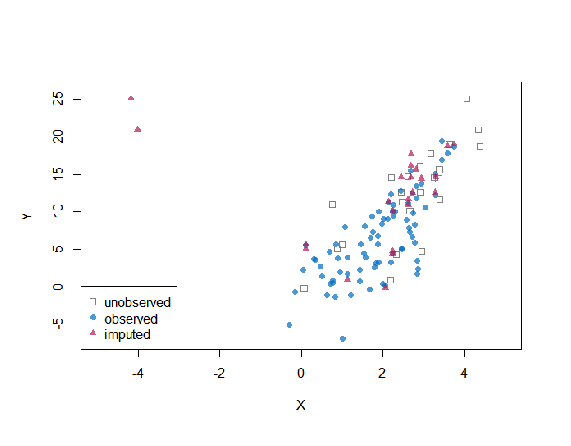
\includegraphics[width=\textwidth, height=10cm]{plots/plot2.1.eps} \\
			\textnormal{(a)}  \\[6pt]
		\end{tabular}
		\begin{tabular}{c}
			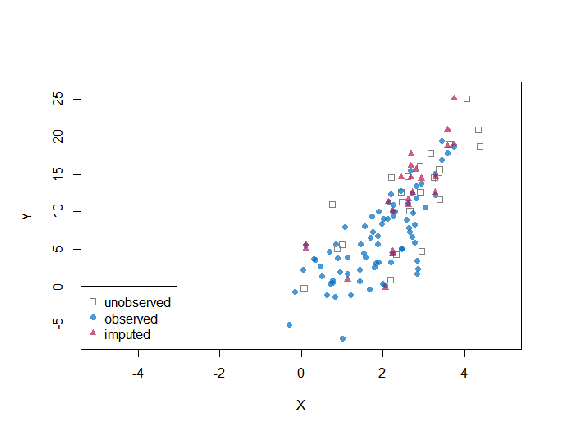
\includegraphics[width=\textwidth, height=10cm]{plots/plot2.2.eps}\\			
			\textnormal{(b)} \\[6pt]
		\end{tabular}
		\caption{Imputations (triangles) generated by OPC and MPC. We see that in (a) some imputations fall outside of the range of the observed (circle) and unobserved values (square), due to the OPC algorithm assigning the donor values to the incorrect distinct real root. In (b) the MPC approach assigns the imputations to the distinct real root that corresponds to the observed and unobserved data.}
		\label{fig2_1}
	\end{figure}
	
	
	\begin{figure}[ht!]
		\begin{tabular}{c}
			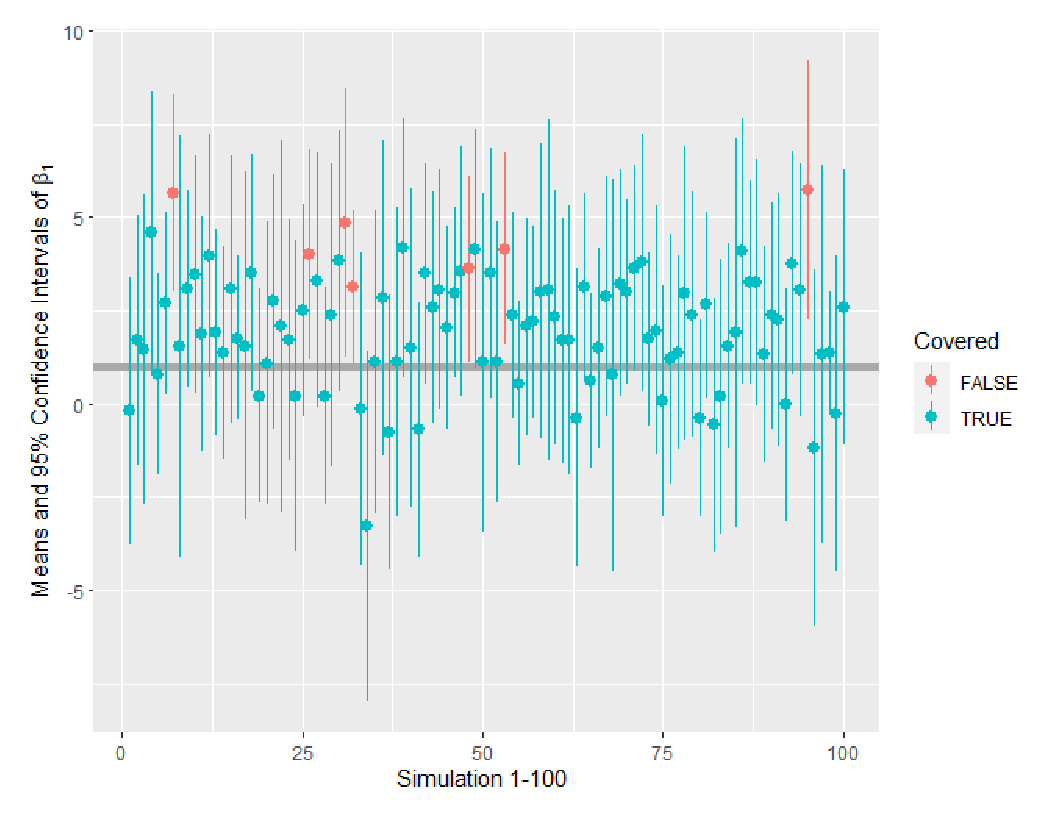
\includegraphics[width=\textwidth, height=10cm]{plots/plot2.3.eps} \\
			\textnormal{(a)}  \\[6pt]
		\end{tabular}
		\begin{tabular}{c}
			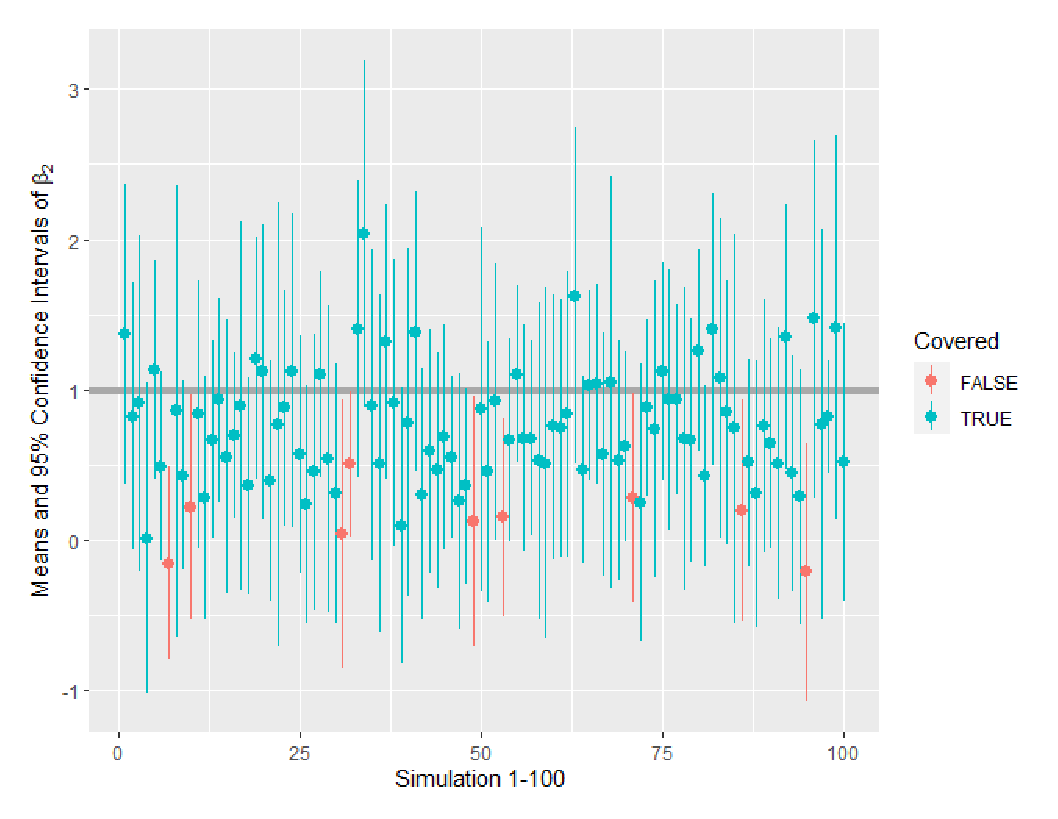
\includegraphics[width=\textwidth, height=10cm]{plots/plot2.4.eps}\\	
			\textnormal{(b)} \\[6pt]
		\end{tabular}
		\caption{The plot of means and confidence intervals of $\beta_{1}$ and $\beta_{2}$ from the first 100 simulations. The model of interest is $Y = X + X^2 + \epsilon$, where $X \sim \frac{1}{2}N(1.125, 0.234) + \frac{1}{2}N(2.875, 0.234)$. The missingness mechanism is MARright and the imputation approach is SMC-FCS. The imputations seem to primarily overestimate the true parameter estimate of $\beta_{1}$ in (a) and underestimate the true parameter estimate of $\beta_{2}$ in (b).}
		\label{fig2_2}
	\end{figure}
	

	\newpage
	\begin{table}[ht!]
		\resizebox{\textwidth}{!}{
			\begin{tabular}{c|ccc|ccc|ccc|ccc|ccc}
				& \multicolumn{15}{c}{Missingness Mechanism}                                                                                           \\
				& \multicolumn{3}{c}{MCAR} & \multicolumn{3}{c}{MARleft} & \multicolumn{3}{c}{MARmid} & \multicolumn{3}{c}{MARtail} & \multicolumn{3}{c}{MARright} \\
				& Bias    & Cov    & Ciw    & Bias    & Cov    & Ciw    & Bias    & Cov    & Ciw    & Bias    & Cov    & Ciw    & Bias   & Cov    & Ciw    \\
				\hline
				Normal         &        &        &        &        &        &        &        &        &        &        &        &        &        &        &        \\
				\texttt{TTI}            &        &        &        &        &        &        &        &        &        &        &        &        &        &        &        \\
				$\beta_1$      & 0.01  & 0.94  & 0.52  & -0.05  & 0.92  & 0.47  & -0.01  & 0.96   & 0.51  & 0.11  & 0.88  & 0.63  & 0.21  & 0.78  & 0.74  \\
				$\beta_2$      & 0  & 0.94  & 0.39  & -0.06  & 0.9  & 0.34  & -0.03  & 0.93  & 0.36  & 0.1  & 0.86  & 0.51  & 0.2  & 0.73  & 0.62  \\
				\texttt{ITT}            &        &        &        &        &        &        &        &        &        &        &        &        &        &        &        \\
				$\beta_1$      & -0.05  & 0.9  & 0.9  & -0.02  & 0.98  & 0.94  & -0.09  & 0.98   & 0.86  & -0.04  & 0.99  & 1.09  & -0.04  & 0.98  & 1.13  \\
				$\beta_2$      & -0.25  & 0.88  & 0.89  & -0.25  & 0.86  & 0.86  & -0.2  & 0.9  & 0.78  & -0.34  & 0.84  & 1.17  & -0.31  & 0.87  & 1.16  \\
				\texttt{OPC}            &        &        &        &        &        &        &        &        &        &        &        &        &        &        &        \\
				$\beta_1$      & 0.03  & 0.94  & 0.56  & 0.01  & 0.95  & 0.46  & 0.01  & 0.95   & 0.48  & 0.08  & 0.87  & 0.75  & 0.09  & 0.88  & 0.87  \\
				$\beta_2$      & 0.03  & 0.92  & 0.41  & 0  & 0.94  & 0.33  & 0  & 0.94  & 0.34  & 0.13  & 0.84  & 0.6  & 0.15  & 0.83  & 0.72  \\
				\texttt{MPC}            &        &        &        &        &        &        &        &        &        &        &        &        &        &        &        \\
				$\beta_1$      & 0.03  & 0.94  & 0.56  & 0.01  & 0.95  & 0.46  & 0.01      & 0.95  & 0.47  & 0.1  & 0.86  & 0.75  & 0.1  & 0.88  & 0.86  \\
				$\beta_2$      & 0.03  & 0.92  & 0.41  & 0  & 0.94  & 0.33  & 0  & 0.94  & 0.34  & 0.13   & 0.84  & 0.6  & 0.15  & 0.83  & 0.72  \\
				\texttt{SMC-FCS}        &        &        &        &        &        &        &        &        &        &        &        &        &        &        &        \\
				$\beta_1$      & 0  & 0.96  & 0.53  & -0.01  & 0.95  & 0.47  & 0.01  & 0.94  & 0.49  & 0  & 0.96  & 0.6  & 0  & 0.95  & 0.67  \\
				$\beta_2$      & 0  & 0.95  & 0.39  & 0  & 0.95  & 0.33  & 0  & 0.95  & 0.34  & 0.01  & 0.95  & 0.51  & 0.02  & 0.95  & 0.57  \\
				\hline
				Skewed-normal    &        &        &        &        &        &        &        &        &        &        &        &        &        &        &        \\
				\texttt{TTI}            &        &        &        &        &        &        &        &        &        &        &        &        &        &        &        \\
				$\beta_1$      & -0.15  & 0.95  & 3.21  & -0.25  & 0.92  & 2.98  & 0.15  & 0.95   & 2.79  & -0.43  & 0.92  & 4.93  & -0.26  & 0.94  & 5.75  \\
				$\beta_2$      & 0.09  & 0.94  & 1.48  & 0.04  & 0.93  & 1.28  & -0.09  & 0.94  & 1.23  & 0.35  & 0.88  & 2.59  & 0.39  & 0.91  & 3.28  \\
				\texttt{ITT}            &        &        &        &        &        &        &        &        &        &        &        &        &        &        &        \\
				$\beta_1$      & 0.3  & 0.94  & 2.55  & 0.27  & 0.93  & 2.24  & 0.18  & 0.96   & 2.39  & 0.5  & 0.9  & 2.91  & 0.41  & 0.94  & 3.18  \\
				$\beta_2$      & -0.13  & 0.96  & 1.27  & -0.12  & 0.93  & 1.01  & -0.07  & 0.96  & 1.07  & -0.24  & 0.9  & 1.71  & -0.15  & 0.95  & 1.91  \\
				\texttt{OPC}            &        &        &        &        &        &        &        &        &        &        &        &        &        &        &        \\
				$\beta_1$      & 0  & 0.93  & 2.68  & -0.02  & 0.94   & 2.49  & 0.03  & 0.93  & 2.4  & -0.07  & 0.86  & 3.64  & 0.01  & 0.82  & 3.79   \\
				$\beta_2$      & 0.03  & 0.92  & 1.27  & 0.01  & 0.94  & 1.11  & -0.01  & 0.94  & 1.08  & 0.16  & 0.85  & 1.98  & 0.13  & 0.82  & 2.16   \\
				\texttt{MPC}            &        &        &        &        &        &        &        &        &        &        &        &        &        &        &        \\
				$\beta_1$      & 0.01  & 0.95  & 2.69  & -0.02  & 0.94  & 2.47  & 0.03  & 0.93  & 2.39  & -0.02  & 0.92  & 3.87  & 0.03  & 0.88  & 4  \\
				$\beta_2$      & 0.03  & 0.94  & 1.29  & 0.01  & 0.94  & 1.11  & -0.01   & 0.93  & 1.08  & 0.15  & 0.91  & 2.09  & 0.15  & 0.86  & 2.26  \\
				\texttt{SMC-FCS}        &        &        &        &        &        &        &        &        &        &        &        &        &        &        &        \\
				$\beta_1$      & -0.14  & 0.94  & 2.59  & -0.01  & 0.95  & 2.39  & -0.15  & 0.96  & 2.43  & -0.41   & 0.93  & 3.51  & -0.49  & 0.91  & 3.56  \\
				$\beta_2$      & 0.09  & 0.95  & 1.21  & 0  & 0.94  & 1.08  & 0.07  & 0.96  & 1.07  & 0.28  & 0.91  & 1.87  & 0.39  & 0.88  & 1.97  \\
				\hline
				Normal-mixture &        &        &        &        &        &        &        &        &        &        &        &        &        &        &        \\
				\texttt{TTI}            &        &        &        &        &        &        &        &        &        &        &        &        &        &        &        \\
				$\beta_1$      & 0  & 0.96  & 0.4  & -0.05  & 0.93  & 0.38  & 0  & 0.95   & 0.4  & 0.02  & 0.95  & 0.43  & 0.1  & 0.86  & 0.46  \\
				$\beta_2$      & 0  & 0.96  & 0.46  & -0.05  & 0.94  & 0.42  & -0.04  & 0.95  & 0.44  & 0.02  & 0.96  & 0.52  & 0.09  & 0.91  & 0.57  \\
				\texttt{ITT}            &        &        &        &        &        &        &        &        &        &        &        &        &        &        &        \\
				$\beta_1$      & -0.04  & 0.98  & 0.62  & 0.03  & 0.98  & 0.59  & -0.02  & 0.98   & 0.58  & -0.07  & 0.98  & 0.65  & -0.09  & 0.98  & 0.68  \\
				$\beta_2$      & -0.42  & 0.59  & 0.98  & -0.36  & 0.71  & 0.96  & -0.32  & 0.72  & 0.86  & -0.55  & 0.35  & 0.97  & -0.52  & 0.4  & 0.96  \\ 
				\texttt{OPC}            &        &        &        &        &        &        &        &        &        &        &        &        &        &        &        \\
				$\beta_1$      & 0.02   & 0.94   & 0.38  & 0  & 0.93  & 0.36  & 0.01  & 0.94  & 0.37  & 0.06  & 0.88  & 0.44  & 0.08  & 0.87  & 0.48  \\
				$\beta_2$      & 0.01  & 0.94  & 0.44  & 0      & 0.93  & 0.41    & 0  & 0.94  & 0.41  & 0.04  & 0.92  & 0.53  & 0.05  & 0.92  & 0.58  \\
				\texttt{MPC}            &        &        &        &        &        &        &        &        &        &        &        &        &        &        &        \\
				$\beta_1$      & 0.02  & 0.94   & 0.38  & 0  & 0.93  & 0.36  & 0.01  & 0.94  & 0.36  & 0.06  & 0.89  & 0.44  & 0.08  & 0.87  & 0.48  \\
				$\beta_2$      & 0.01  & 0.95  & 0.44  & 0  & 0.94  & 0.41  & 0  & 0.94  & 0.4  & 0.04  & 0.92  & 0.53  & 0.05  & 0.93  & 0.58  \\
				\texttt{SMC-FCS}        &        &        &        &        &        &        &        &        &        &        &        &        &        &        &        \\
				$\beta_1$      & -0.01  & 0.95  & 0.4  & -0.02  & 0.95  & 0.38  & 0.02  & 0.95  & 0.38  & -0.05  & 0.93  & 0.43  & -0.05  & 0.93  & 0.48  \\
				$\beta_2$      & -0.02  & 0.95  & 0.46   & 0.01  & 0.94  & 0.41   & -0.03  & 0.94  & 0.42  & -0.03  & 0.94  & 0.51  & -0.06  & 0.93  & 0.57 
			\end{tabular}
		}
		\caption{Simulation results for five missingness mechanisms when imputing a squared term regression where the mean of X equals 0. Shown are the absolute bias of the estimate, coverage of the 95\% confidence interval for the estimate and the average confidence interval width.}
		\label{tab2_3}
	\end{table}
	
	\newpage
	\begin{table}[ht!]
		\resizebox{\textwidth}{!}{
			\begin{tabular}{c|ccc|ccc|ccc|ccc|ccc}
				& \multicolumn{15}{c}{Missingness Mechanism}                                                                                               \\
				& \multicolumn{3}{c}{MCAR} & \multicolumn{3}{c}{MARleft} & \multicolumn{3}{c}{MARmid} & \multicolumn{3}{c}{MARtail} & \multicolumn{3}{c}{MARright} \\
				& Bias     & Cov    & Ciw    & Bias     & Cov    & Ciw    & Bias     & Cov    & Ciw    & Bias     & Cov    & Ciw    & Bias    & Cov    & Ciw    \\ \hline
				Normal                            &         &        &        &         &        &        &         &        &        &         &        &        &         &        &        \\
				\texttt{TTI}            &        &        &        &        &        &        &        &        &        &        &        &        &        &        &        \\
				$\beta_1$      & -0.58  & 0.93  & 7.17  & -1  & 0.92  & 8  & -0.08  & 0.95   & 6.04  & -1.32  & 0.91  & 10.11  & -0.89  & 0.93  & 9.24  \\
				$\beta_2$      & 0.11  & 0.93  & 1.66  & 0.15  & 0.93  & 1.73  & 0  & 0.95  & 1.39  & 0.31  & 0.89  & 2.43  & 0.29  & 0.91  & 2.4  \\
				\texttt{ITT}            &        &        &        &        &        &        &        &        &        &        &        &        &        &        &        \\
				$\beta_1$      & 0.71  & 0.94  & 5.61  & 0.6  & 0.94  & 5.57  & 0.5  & 0.96   & 5.27  & 0.99  & 0.92  & 5.95  & 1.02  & 0.93  & 4.97  \\
				$\beta_2$      & -0.19  & 0.95  & 1.41  & -0.14  & 0.95  & 1.31  & -0.13  & 0.96  & 1.28  & -0.28  & 0.9  & 1.58  & -0.3  & 0.91  & 1.63  \\
				\texttt{OPC}     &         &        &        &         &        &        &         &        &        &         &        &        &         &        &        \\
				$\beta_1$                         & -0.05  & 0.92  & 5.28  & -0.15   & 0.93  & 5.56  & 0.01   & 0.93  & 4.98  & -0.12   & 0.87  & 6.04  & 0.04   & 0.8  & 5.65  \\
				$\beta_2$                         & 0.02    & 0.93  & 1.27  & 0.03   & 0.94  & 1.27  & 0   & 0.94  & 1.17  & 0.05   & 0.87  & 1.51  & 0.03   & 0.82  & 1.48  \\
				\texttt{MPC}     &         &        &        &         &        &        &         &        &        &         &        &        &         &        &        \\
				$\beta_1$                         & -0.05   & 0.93  & 5.17  & -0.15   & 0.94  & 5.39  & 0   & 0.91  & 4.77  & -0.03   & 0.93  & 6.26  & 0.05   & 0.89  & 6.02  \\
				$\beta_2$                         & 0.02   & 0.93  & 1.25  & 0.03   & 0.94  & 1.24  & 0.01   & 0.92  & 1.13  & 0.04   & 0.91  & 1.56  & 0.04   & 0.88  & 1.57  \\
				\texttt{SMC-FCS} &         &        &        &         &        &        &         &        &        &         &        &        &         &        &        \\
				$\beta_1$                         & 0.03    & 0.95   & 5.44  & -0.11   & 0.95  & 5.78   & -0.06   & 0.95  & 5.14  & -0.22   & 0.94  & 6.02  & -0.1   & 0.97  & 5.69  \\
				$\beta_2$                         & 0   & 0.95  & 1.3  & 0.03   & 0.94  & 1.31  & 0.01   & 0.95  & 1.25  & 0.06    & 0.94  & 1.5  & 0.04   & 0.96  & 1.48  \\ \hline
				Skewed-normal                       &         &        &        &         &        &        &         &        &        &         &        &        &         &        &        \\
				\texttt{TTI}            &        &        &        &        &        &        &        &        &        &        &        &        &        &        &        \\
				$\beta_1$      & -0.15  & 0.93  & 2.95  & -0.45  & 0.92  & 4.14  & -0.06  & 0.95   & 2.56  & -0.32  & 0.95  & 4.07  & -0.07  & 0.94  & 2.97  \\
				$\beta_2$      & 0.06  & 0.93  & 1.27  & 0.14  & 0.92  & 1.59  & 0.03  & 0.95  & 1.11  & 0.12  & 0.94  & 1.73  & 0.06  & 0.93  & 1.41  \\
				\texttt{ITT}            &        &        &        &        &        &        &        &        &        &        &        &        &        &        &        \\
				$\beta_1$      & 0.46  & 0.92  & 2.64  & 0.29  & 0.93  & 2.86  & 0.35  & 0.94   & 2.49  & 0.62  & 0.87  & 2.83  & 0.73  & 0.81  & 2.48  \\
				$\beta_2$      & -0.28  & 0.88  & 1.26  & -0.13  & 0.94  & 1.23  & -0.21  & 0.9  & 1.16  & -0.37  & 0.8  & 1.37  & -0.48  & 0.64  & 1.26  \\
				\texttt{OPC}     &         &        &        &         &        &        &         &        &        &         &        &        &         &        &        \\
				$\beta_1$                         & 0.01   & 0.92  & 2.24  & -0.11   & 0.93  & 2.74   & 0.02   & 0.93  & 2.19  & -0.07   & 0.88  & 2.5  & 0   & 0.85  & 2.19  \\
				$\beta_2$                         & 0   & 0.93  & 0.99  & 0.05    & 0.93  & 1.14  & -0.01   & 0.94  & 0.96  & 0.04    & 0.89  & 1.11  & 0.02   & 0.86  & 1.03  \\
				\texttt{MPC}     &         &        &        &         &        &        &         &        &        &         &        &        &         &        &        \\
				$\beta_1$                         & 0   & 0.92  & 2.18  & -0.11   & 0.93  & 2.66  & 0   & 0.92  & 2.02  & -0.04    & 0.94  & 2.59  & 0.02   & 0.91  & 2.28  \\
				$\beta_2$                         & 0.01   & 0.93   & 0.96  & 0.05   & 0.93  & 1.11  & 0   & 0.93  & 0.89  & 0.04   & 0.95  & 1.15  & 0.02   & 0.9   & 1.06  \\
				\texttt{SMC-FCS} &         &        &        &         &        &        &         &        &        &         &        &        &         &        &        \\
				$\beta_1$                         & 0.1   & 0.95  & 2.46  & -0.04   & 0.95  & 3.01  & 0.09    & 0.95  & 2.27  & 0.14   & 0.95  & 2.65  & 0.2     & 0.93  & 2.22  \\
				$\beta_2$                         & -0.05   & 0.94  & 1.08  & 0.03  & 0.95  & 1.22  & -0.04   & 0.94  & 1  & -0.08   & 0.94  & 1.2    & -0.14   & 0.91  & 1.04  \\ \hline
				Normal-mixture                    &         &        &        &         &        &        &         &        &        &         &        &        &         &        &        \\
				\texttt{TTI}            &        &        &        &        &        &        &        &        &        &        &        &        &        &        &        \\
				$\beta_1$      & -1.5  & 0.9  & 10.48  & -2.15  & 0.86  & 11.93  & -0.71  & 0.93   & 8.8  & -2.35  & 0.87  & 13.63  & -1.73  & 0.91  & 12.47  \\
				$\beta_2$      & 0.33  & 0.9  & 2.52  & 0.43  & 0.87  & 2.73  & 0.16  & 0.94  & 2.11  & 0.51  & 0.88  & 3.29  & 0.43  & 0.9  & 3.15  \\
				\texttt{ITT}            &        &        &        &        &        &        &        &        &        &        &        &        &        &        &        \\
				$\beta_1$      & 1.38  & 0.88  & 6.4  & 0.83  & 0.92  & 6.13  & 1.07  & 0.92   & 6.33  & 1.76  & 0.8  & 6.08  & 2.08  & 0.78  & 6.35  \\
				$\beta_2$      & -0.35  & 0.88  & 1.62  & -0.19  & 0.94  & 1.52  & -0.25  & 0.92  & 1.58  & -0.49  & 0.76  & 1.57  & -0.57  & 0.72  & 1.63  \\	
				\texttt{OPC}     &         &        &        &         &        &        &         &        &        &         &        &        &         &        &        \\
				$\beta_1$                         & -0.05  & 0.92  & 6.28  & -0.24   & 0.92  & 6.51  & 0.02   & 0.93  & 6.05  & -0.09   & 0.88  & 6.61  & 0.19    & 0.85  & 6.43  \\
				$\beta_2$                         & 0.02    & 0.92   & 1.53  & 0.06   & 0.92  & 1.57  & 0   & 0.94  & 1.47   & 0.04   & 0.87  & 1.64  & -0.03   & 0.86  & 1.62  \\
				\texttt{MPC}     &         &        &        &         &        &        &         &        &        &         &        &        &         &        &        \\
				$\beta_1$                         & -0.04   & 0.93  & 6.24  & -0.23   & 0.92   & 6.39  & 0.02  & 0.91  & 5.92  & -0.04  & 0.93  & 6.77  & 0.24   & 0.92  & 6.69   \\
				$\beta_2$                         & 0.02   & 0.93  & 1.53  & 0.05    & 0.93  & 1.54  & 0   & 0.92   & 1.45  & 0.03   & 0.92   & 1.68  & -0.03   & 0.92   & 1.69  \\
				\texttt{SMC-FCS} &         &        &        &         &        &        &         &        &        &         &        &        &         &        &        \\
				$\beta_1$                         & 0.32   & 0.95  & 6.37  &-0.32   & 0.96  & 6.85   & 0.25   & 0.94  & 6.18  & 0.5   & 0.94  & 6.58  & 0.95   & 0.91  & 6.69  \\
				$\beta_2$                         & -0.07   & 0.94  & 1.57  & 0.09   & 0.95   & 1.65  & -0.04   & 0.94  & 1.5  & -0.14   & 0.92   & 1.66  & -0.25   & 0.9  & 1.71 
			\end{tabular}
		}
		\caption{Simulation results for five missingness mechanisms when imputing a squared term regression where the mean of X equals 2. Shown are the absolute bias of the estimate, coverage of the 95\% confidence interval for the estimate and the average confidence interval width.}
		\label{tab2_4}
	\end{table}



		\chapter{Generalizing univariate predictive mean matching to impute multiple variables simultaneously}
\label{chap3}
	\begin{abstract}
		Predictive mean matching (PMM) is an easy-to-use and versatile univariate imputation approach. It is robust against transformations of the incomplete variable and violation of the normal model. However, univariate imputation methods cannot directly preserve multivariate relations in the imputed data. We wish to extend PMM to a multivariate method to produce imputations that are consistent with the knowledge of derived data (e.g., data transformations, interactions, sum restrictions, range restrictions, and polynomials). This paper proposes multivariate predictive mean matching (MPMM), which can impute incomplete variables simultaneously. Instead of the normal linear model, we apply canonical regression analysis to calculate the predicted value used for donor selection. To evaluate the performance of MPMM, we compared it with other imputation approaches under four scenarios: 1) multivariate normal distributed data, 2) linear regression with quadratic terms; 3) linear regression with interaction terms; 4) incomplete data with inequality restrictions. The simulation study shows that with moderate missingness patterns, MPMM provides plausible imputations at the univariate level and preserves relations in the data.   
	\end{abstract}

	\section{Introduction}
	\label{sec:3.1}
	Multiple imputation (MI) is a popular statistical method for the analysis of missing data problems. To provide valid inferences from the incomplete data, the analysis procedure of MI consists of three steps. First, in the imputation step, missing values are drawn from a plausible distribution (e.g., posterior distributions for Bayesian model-based approaches and a cluster of candidate donors for non-parametric approaches) to generate several (\emph{m}) complete datasets. The value of \emph{m} commonly varies between 3 to 10. Second, in the analysis step, complete data analysis are used to estimate the quantity of scientific interest for each imputed data set. This step yields \emph{m} separate analyses because imputed datasets are different. Finally, in the pooling step, m results are aggregated into a single result by Rubin’s rules, accounting for the uncertainty of estimates due to the missing data \citep[p.76]{RubinD1987}. 
	
	Two widely used strategies for imputing multivariate missing data are joint modeling (JM) and fully conditional specification (FCS). Joint modeling was proposed by \citet{RubinD1987} and especially developed by \citet{schafer1997analysis}. Given that the data is assumed to follow a multivariate distribution, all incomplete variables are generally imputed by drawing from the joint posterior predictive distribution conditional on other variables. Fully conditional specification, which was developed by \citet{van2007multiple}, follows an iterative scheme that imputes each incomplete variable based on a conditionally specified model. Fully conditional specification allows for tremendous flexibility in multivariate model design and flexibility in imputing non-normal variables, especially discrete variables \citep{goldstein2014fitting}. However, FCS may suffer from incompatibility problems, and computational shortcuts like the sweep operator cannot be applied to facilitate computation \citep{Buuren2018}. On the other hand, joint modeling possesses more solid theoretical guarantees. With increasing incomplete variables, JM may lead to unrealistically large models and a lack of flexibility, which will not occur under FCS.  
	
	In practice, there are often extra structures in the missing data which are not modelled properly. Suppose there are two jointly missing variables $\boldsymbol{X_1}$ and $\boldsymbol{X_2}$. There may be restrictions on the sum of $\boldsymbol{X_1}$ and $\boldsymbol{X_1}$ (e.g., $\boldsymbol{X_1} + \boldsymbol{X_1} = C$, where $C$ is a fixed value) and the rank of $\boldsymbol{X_1}$ and $\boldsymbol{X_2}$ (e.g., $\boldsymbol{X_1} > \boldsymbol{X_2}$), data transformations (e.g., $\boldsymbol{X_2} = log(\boldsymbol{X_1})$, $\boldsymbol{X_2} = \boldsymbol{X_1}^2$) or interaction terms included in the data ($\boldsymbol{X_1}$, $\boldsymbol{X_2}$, $\boldsymbol{X_3}$ are jointly missing, where $\boldsymbol{X_3} = \boldsymbol{X_1} * \boldsymbol{X_2}$). In this paper, we would focus on the setting of structures between two jointly missing variables, which is a simple scenario to illustrate.  
	
	The two popular approaches of MI mentioned before may not be appropriate for modeling the relations among multiple variables in the missing data. Joint modeling may lack the flexibility of modeling the relations explicitly, and FCS imputes each missing variable separately, which may not ensure that the imputation remains consistent with the observed relations among multiple variables. 
	
	\citet[section 4.7.2]{Buuren2018} suggested block imputation, which combines the strong points of joint modeling and fully conditional specification. The general idea is to place incomplete variables into blocks and apply multivariate imputation methods to the block. Joint modeling can be viewed as a ``single block" imputation method. In contrast, FCS is strictly a multiple blocks imputation method, where the number of blocks equals the number of incomplete columns in the data. It is feasible to consider the relations among a set of missing variables if we specify them as a single block and perform the MI iteratively over the blocks. 
	
	Based on the rationale of block imputation, we extend univariate predictive mean matching to the multivariate case to allow for the joint imputation of blocks of variables. The general idea is to match the incomplete case to one of the complete cases by applying canonical regression analysis and imputing the variables in a block entirely from the matched case \citep{little1988missing}. We shall refer to the multivariate extension of PMM as \emph{multivariate predictive mean matching} (MPMM).  
	
	Predictive mean matching (PMM) is a user-friendly and versatile non-parametric imputation method. Multiple imputation by chained equation (\texttt{MICE}), which is a popular software package in \texttt{R} for imputing incomplete multivariate data by Fully Conditional Specification (FCS), sets the PMM as the default imputation approach \citep{Buuren2011}. We tailor PMM to the block imputation framework, which will widen its application. More computational details and properties of PMM would be addressed in section \ref{sec:3.2}.       
	
	
	For a comprehensive overview of missing data analysis, we refer to \citet{little2019statistical} for a comparison of approaches to missing data other than multiple imputation (e.g, ad-hoc methods, maximum likelihood estimation and weighting methods). \citet{schafer1999multiple}, \citet{sinharay2001use} and \citet{allison2001missing} introduced basic concepts and general methods of MI. \citet{schafer2002missing} discussed practical issues of application of MI. Various sophisticated missing data analysis were developed on the fields of multilevel model \citep{longford2001multilevel}, structural equation modeling \citep{olinsky2003comparative, allison2003missing}, longitudinal data analysis \citep{twisk2002attrition, demirtas2004modeling} and meta-analysis \citep{pigott2001missing}. \citet{schafer2003multiple} compared Bayesian MI methods with maximum likelihood estimation. \citet{seaman2013review} gave an overview of the use of inverse probability weighting in missing data problems. \citet{ibrahim2005missing} provided a review of various advanced missing data methods. Because an increasing number of missing data methodologies emerged, MI as well as other approaches were applied in many fields (e.g., epidemiology, psychology and sociology) and implemented in many statistical software packages (e.g., \texttt{mice} and \texttt{mi} in \texttt{R}, \texttt{IVEWARE} in \texttt{SAS}, \texttt{ice} in \texttt{STATA} and module \texttt{MVA} in \texttt{SPSS}) \citep{Buuren2011}.
	
	
	
	The following section will outline canonical regression analysis, introduce predictive mean matching (PMM), and connect the techniques to propose multivariate predictive mean matching (MPMM). Section \ref{sec:3.3} provides a simple comparison between PMM and MPMM. Section \ref{sec:3.4} is a simulation study investigating whether MPMM yields valid estimates and preserves functional relations between imputed values. The discussion closes the paper.
	
	
	
	
	
	\section{Multivariate Predictive Mean Matching}
	\label{sec:3.2}
	\subsection{Canonical regression analysis (CRA)}
	Canonical regression analysis is a derivation and an asymmetric version of canonical correlation analysis (CCA). It aims to look for a linear combination of covariates that predicts a linear combination of outcomes optimally in a least-squares sense \citep{Israels1987}. The basic idea of canonical regression analysis is quite old and has been discussed under different names, such as Rank-reduced regression \citep{izenman1975reduced} and partial least squares \citep{sun2009equivalence}.  
	
	Let us consider the equation
	\begin{equation}
		\boldsymbol{\alpha'Y} = \boldsymbol{\beta X} + \epsilon.
	\end{equation}
	We aim to minimize the variance $\epsilon$ with respect to $\alpha$ and $\beta$ under some restrictions. CRA can be implemented by maximizing the squared multiple correlation coefficient for the regression of $\alpha'Y$ on $X$, which can be written as
	\begin{equation}
		R^2_{\alpha'y.x}=\frac{\boldsymbol{\alpha'\Sigma_{yx}\Sigma^{-1}_{xx}\Sigma_{xy}\alpha}}{\boldsymbol{\alpha'\Sigma_{yy}\alpha}},
	\end{equation}
	where $R^2_{\alpha'y.x}$ is the ratio of the amount of variance of $\boldsymbol{\alpha'Y}$ accounted for by the covariates $\boldsymbol{X}$ to the total variance. According to \citet{McDonald1968}, maximization of the above equation leads to eigenvalue decomposition. The solution is that $\boldsymbol{\alpha}$ is the right-hand eigenvector of $\boldsymbol{\Sigma^{-1}_{yy}\Sigma_{yx}\Sigma^{-1}_{xx}\Sigma_{xy}}$ corresponding to its greatest eigenvalue. After reducing the rank of $\boldsymbol{\alpha'Y}$ to $1$, we could estimate $\boldsymbol{\beta}$ by multivariate regression analysis. 
	
	\subsection{Predictive mean matching (PMM)}
	PMM was first proposed by \citet{rubin1986statistical}and formalized by \citet{little1988missing}. It can be viewed as an extension of the $k$ nearest neighbor method. PMM calculates the estimated value of the missing variable through a specified imputation model (e.g., linear imputation model). The method selects a set of candidate donors (typically, the number of candidate donors is 5) from all complete cases whose estimated values are closest to the estimated value of the missing unit. The unobserved value is imputed by randomly drawing one of the observed values of the candidate donors \citep{Buuren2018}.
	
	\subsubsection{Computational details}
	We elaborate the algorithm of predictive mean matching for the clear illustration of its merger with canonical regression analysis \citep{Vink2015}. $\boldsymbol{X_{obs}}$, a $N_{obs} \times j$ matrix, denotes the observed part of predictors and $\boldsymbol{X_{mis}}$, a $N_{mis} \times j$ matrix, denotes the missing part of predictors. 
	\begin{enumerate}
		\item Use linear regression of $\boldsymbol{Y_{obs}}$ given $\boldsymbol{X_{obs}}$ to estimate $\boldsymbol{\hat{\beta}}$ and $\hat{\epsilon}$ through ordinary least squares
		\item Draw $\sigma^{2\ast}=\hat{\epsilon}^\mathsf{T}\hat{\epsilon}/A$, where $A$ is a $\chi^2$ variate with $N_{obs}-j$ degrees of freedom
		\item Draw $\boldsymbol{\beta^{\ast}}$ from a multivariate normal distribution with mean vector $\boldsymbol{\hat{\beta}}$ and covariance matrix $\boldsymbol{\sigma^{2\ast}(X^\mathsf{T}_{obs}X_{obs})^{-1}}$
		\item Calculate $\boldsymbol{\hat{V}_{obs}=X_{obs}\hat{\beta}}$ and $\boldsymbol{\hat{V}_{mis}=X_{mis}\beta^{\ast}}$
		\item For each missing cell $y_{mis,n}$, where $n=1,\cdots,N_{mis}$
		\begin{enumerate}
			\item Find $\Delta=|\hat{v}_{mis,n}-\hat{v}_{obs,k}|$ for all $k=1,\cdots,N_{obs}$
			\item Pick several observed entries $y_{obs}$, 5 as default in \emph{mice.impute.pmm}, with the smallest distance defined in step 5(a)
			\item Randomly draw one of the $y_{obs}$ which are picked in the previous step to impute $y_{mis,n}$  
		\end{enumerate}
		\item Repeat steps 1-5 \emph{m} times and save \emph{m} completed datasets. 
	\end{enumerate}
	
	Predictive mean matching has been proven to perform well in a wide range of simulation studies and is an attractive way to impute missing data \citep{Buuren2011, Vink2015, Heitjan1991, Morris2014, Vink2014}. More precisely, PMM has the appealing features that the imputed values 1) follow the potential distributions of the data and 2) are always within the range of observed data because imputed values are replaced by real observed values \citep{Buuren2018}. For the same reason, PMM yields acceptable imputations even when normality assumptions are violated \citep{Vink2014}. In cases where the observed values follow a skewed distribution, the imputations will also be skewed. If observations are strictly positive, so will the imputations from PMM be. Furthermore, since PMM does not rely on model assumptions, it alleviates the adverse impact when the imputation model is misspecified \citep{JamesR.Carpenter2013}. 
	
	Although PMM was developed for situations with only a single incomplete variable, it is easy to implement it under a fully conditionally specification framework for imputing multivariate missing data. However, the application of PMM under FCS framework is only limited to univariate imputation. Therefore, it may distort the multivariate relations in the imputations and narrow the application of the method to more complex data structures. For example, \citet{seaman2012multiple} concluded that a univariate implementation of predictive mean matching is not advised to produce plausible estimates when the analysis model contains non-linear terms. As a multivariate extension to PMM, we expect that MPMM could yield plausible and consistent imputations when missing covariates include polynomial or interaction terms.  
	
		
	\subsection{Multivariate predictive mean matching (MPMM)}
	\label{sec:3.2.3}
	For illustration, we present the algorithm with one missing data pattern. The appendix discusses the extension to cases with multiple missing patterns. 
	Let $\boldsymbol{Y=(Y_1,\cdots,Y_I)}$ and $\boldsymbol{X=(X_1,\cdots,X_J)}$ be two sets of $I$ jointly incomplete variables and $J$ complete  quantitative variables, respectively. Let $\boldsymbol{V = \alpha Y}$ denotes the linear combination of multiple response variables and $\boldsymbol{X}$ denotes predictors with $j$ dimensions. 
	\begin{enumerate}
		\item Use the observed data to estimate the $(I+J)\times(I+J)$ covariance matrix
		\[ \left( \begin{array}{cc}
			\boldsymbol{\Sigma_{y_{obs}y_{obs}}} & \boldsymbol{\Sigma_{y_{obs}x_{obs}}}  \\
			\boldsymbol{\Sigma_{x_{obs}y_{obs}}} & \boldsymbol{\Sigma_{x_{obs}x_{obs}}}  \end{array} \right)\]
		\item Find the largest eigenvalue $\lambda^2$ of $\boldsymbol{\Sigma^{-1}_{y_{obs}y_{obs}}\Sigma_{y_{obs}x_{obs}}\Sigma^{-1}_{x_{obs}x_{obs}}\Sigma_{x_{obs}y_{obs}}}$ and its corresponding right-hand eigenvector $\alpha$
		\item Calculate the linear combination $\boldsymbol{\alpha'Y}$ for all completely observed individuals in the sample: $\boldsymbol{V_{obs}=\alpha'Y_{obs}}$ 
		\item Use linear regression of $\boldsymbol{V_{obs}}$ given $\boldsymbol{X_{obs}}$ to estimate $\boldsymbol{\hat{\beta}}$ and $\hat{\epsilon}$ through ordinary least squares
		\item Draw $\sigma^{2\ast}=\hat{\epsilon}^\mathsf{T}\hat{\epsilon}/A$, where $A$ is a $\chi^2$ variate with $N_{obs}-j$ degrees of freedom
		\item Draw $\beta^{\ast}$ from a multivariate normal distribution with mean vector $\boldsymbol{\hat{\beta}}$and covariance matrix $\boldsymbol{\sigma^{2\ast}(X^\mathsf{T}_{obs}X_{obs})^{-1}}$
		\item Calculate $\boldsymbol{\hat{V}_{obs}=X_{obs}\hat{\beta}}$ and $\boldsymbol{\hat{V}_{mis}=X_{mis}\beta^{\ast}}$
		\item For each missing vector $\boldsymbol{y_{mis,n}}$, where $n=1,\cdots,N_{mis}$
		\begin{enumerate}
			\item Find $\Delta=|\hat{v}_{mis,n}-\hat{v}_{obs,k}|$ for all $k=1,\cdots,N_{obs}$
			\item Pick several observed components $y_{obs} = \{y_{1, obs},\cdots,y_{I, obs}\}$, 5 as default, with the smallest distance defined in step 8(a)
			\item Randomly draw one of the $y_{obs}$ which are picked in the previous step to impute $y_{mis,n}$ 
		\end{enumerate}
		\item Repeat steps 5-8 \emph{m} times and save \emph{m} completed datasets.
	\end{enumerate}
	
	We also tried other methods of multivariate analysis, such as multivariate regression analysis (MRA) \citep[chapter 10]{rencher2003methods} and redundancy analysis (RA) \citep{van1977redundancy}. However, imputation models specified by MRA or RA are not appropriate because of the assumed independence between missing variables. The violation of this assumption leads to less sensible imputations when there are extra relations among missing covariates. 
	
	\section{Comparison between PMM and MPMM}
	\label{sec:3.3}
	We shall illustrate that although MPMM is a multivariate imputation method, where the whole missing component is assigned entirely from the matching donor, the derived imputed datasets are also plausible at the univariate level. 
	
	\subsection{Simulation conditions}
	The predictors were generated by a multivariate distribution  
	\begin{eqnarray*}
		\begin{pmatrix}\boldsymbol{X_{1}}\\
			\boldsymbol{X_{2}}\\
			\boldsymbol{X_{3}}
		\end{pmatrix} & \sim & \mathcal{N}\left[\left(\begin{array}{c}
			2\\
			2\\
			2
		\end{array}\right),\left(\begin{array}{ccc}
			12 & 0 & 0\\
			0 & 12 & 0\\
			0 & 0 & 12
		\end{array}\right)\right].\\
	\end{eqnarray*}
	The responses were generated based on the multivariate linear model
	\begin{eqnarray*}
		\begin{pmatrix}\boldsymbol{Y_{1}}\\
			\boldsymbol{Y_{2}}\\
			\boldsymbol{Y_{3}}
		\end{pmatrix} & \sim & \mathcal{N}\left[\left(\begin{array}{c}
			3\boldsymbol{X_1} + \boldsymbol{X_2} + 2\boldsymbol{X_{3}}\\
			\boldsymbol{X_{1}} + 5\boldsymbol{X_{2}} + 2\boldsymbol{X_{3}}\\
			5\boldsymbol{X_{1}} + 3\boldsymbol{X_{2}} + \boldsymbol{X_{3}}
		\end{array}\right),\left(\begin{array}{ccc}
			4 & 4\rho & 4\rho\\
			4\rho & 4 & 4\rho\\
			4\rho & 4\rho & 4
		\end{array}\right)\right],\\
	\end{eqnarray*}
	where $\rho$ denotes the correlation between the predictors $\boldsymbol{X}$. Let \textbf{R} be the vector of observation indicators whose values are zero if the corresponding variable is missing and one if observed. We simulated missingness such that rows in the set $(\boldsymbol{Y_1, Y_2, Y_3})$ were always either observed or completely missing. This joint missingness was either completely at random (MCAR) with $P(\textbf{R}=0|\textbf{X}, \textbf{Y})=0.4$ or right-tailed missing at random (MARright) with $P(\textbf{R}=0|\textbf{X}, \textbf{Y})=\frac{\mathrm{e}^a}{1+\mathrm{e}^a}$, where $a=\alpha_0+\boldsymbol{X_1}/SD(\boldsymbol{X_1})$ and $\alpha_0$ was chosen to make the probability of jointly missing \textbf{Y} equal to 0.4. Missing values were induced with the \texttt{ampute} function \citep{Schouten2018} from the package \texttt{MICE} \citep{Buuren2011} in \texttt{R} \citep{R2018}. The correlation $\rho$ was simulated from 0.2, 0.5 or 0.8 corresponding to a weak, moderate and strong dependence between predictors. The sample size was 2000, and 1000 simulations were repeated for different setups. 
	
	For reasons of brevity, we focused our evaluation on the expectation of $\boldsymbol{Y_{1}}$ and the correlation between $\boldsymbol{Y_{1}}$ and $\boldsymbol{Y_{2}}$. We studied the average bias over 1000 simulations with respect to the designed population value and the coverage rate of nominal 95\% confidence interval. Within each simulation, we generated five imputed datasets and combined the statistics into a single inference by using Rubin's combination rules \citep[p.76]{RubinD1987}.  
	
	\subsection{Results}
	\begin{table}[ht!]
		\centering
		\resizebox{\textwidth}{!}{
			\begin{tabular}{ccccc|cc|cc|cc}
				
				\hline
				&&&\multicolumn{4}{c|}{$E(Y_{1})$}&\multicolumn{4}{c}{$\rho(Y_{1}, Y_{2})$}\\
				\cline{3-11}
				&&&\multicolumn{2}{c}{PMM}&\multicolumn{2}{c|}{PMM-CRA}&\multicolumn{2}{c}{PMM}&\multicolumn{2}{c}{PMM-CRA}\\
				\cline{3-11}
				&$\rho$&scenario&bias&cov&bias&cov&bias&cov&bias&cov\\
				\hline
				&\multirow{2}{*}{$0$}
				&MCAR&0&0.94&0&0.95&0&0.95&0&0.94\\
				&&MAR&0&0.93&0&0.94&0&0.96&0&0.94\\	
				\hline
				&\multirow{2}{*}{$0.5$}
				&MCAR&0&0.95&0&0.93&0&0.95&0&0.95\\
				&&MAR&0&0.94&0&0.94&0&0.94&0&0.94\\
				\hline
				&\multirow{2}{*}{$0.8$}
				&MCAR&0&0.93&0&0.94&0.01&0.91&0&0.95\\
				&&MAR&0&0.93&0&0.93&0.01&0.93&0&0.94\\ 
				
			\end{tabular}
			
		}	
		\caption{Simulation results for evaluating whether MPMM provide valid imputations at the univariate level.}
		\label{tab3_1}
	\end{table}   
	
	In general, MPMM yielded no discernible difference with PMM when focusing on the correlation coefficient $\rho(\boldsymbol{Y_{1}}, \boldsymbol{Y_{2}})$. Under the MCAR missingness mechanism, both methods yielded unbiased estimates and displayed coverage rates close to the nominal 95\%, and even there was 40\% missingness in the joint set $(\boldsymbol{Y_1, Y_2, Y_3})$. It is notable to see that with MARright and high correlation between $\boldsymbol{Y_{1}}$ and $\boldsymbol{Y_{2}}$, PMM had a somewhat reduced coverage rate, which suggests that MPMM yielded more robust results against various correlation coefficients. For estimation of the mean value $E(Y_{1})$, MPMM performed similarly to PMM. Both methods yielded plausible imputations with various missingness scenarios and different pre-assumed correlation coefficients. 
	
	These initial results suggested that multivariate predictive mean matching could be an alternative to predictive mean matching. If PMM yields sensible imputations, so will PMM-CRA.
	
	\section{Evaluation}
	\label{sec:3.4}
	To investigate the performance of MPMM when there are relations in the incomplete data, we performed the following simulation studies. 
	
	\subsection{Linear regression with squared term}
	\label{sec:3.4.1}
	We first simulated from a linear regression substantive model with a squared term. 
	\subsubsection{Simulation conditions}
	The dependent variable $\boldsymbol{Y}$ was generated according to the analysis model
	\begin{equation}
		\boldsymbol{Y} = \alpha + \beta_1\boldsymbol{X} + \beta_2 \boldsymbol{X^2} + \epsilon
	\end{equation}
	where $\alpha=0$, $\beta_1=1$, $\beta_2=1$, both predictor $\boldsymbol{X}$ and error term $\epsilon$ were assumed as standard normal distributions. These coefficients lead to a strong quadratic association between $\boldsymbol{Y}$ and $\boldsymbol{X}$. A large sample size ($n=5000$) was created. Simulations were repeated 1000 times so that we could achieve more robust and stable analyses. Forty percent of $\boldsymbol{X}$ and $\boldsymbol{X^2}$ were designed to be jointly missing under five various missingness mechanisms: MCAR, MARleft, MARmid, MARtail, and MARright \footnote[1]{With left-tailed (MARleft), centered (MARmid), both tailed (MARtail) or right-tailed (MARright) missingness mechanism, a higher probability of $\boldsymbol{X}$ being missing are assigned to the units with low, centered, extreme and high values of $Y$ respectively.}, which means no cases with missing values on either $X$ or $X^2$ for each mechanism. Missing values were again created with the \texttt{ampute} function from the package \texttt{MICE} in \texttt{R}.
	
	\subsubsection{Estimation methods}
	We compared the performance of MPMM to four other approaches: \emph{`transform, then impute'} (TTI), \emph{`impute, then transform'} (ITT), polynomial combination method (PC) and substantive model compatible FCS (SMC-FCS). \emph{`Impute, then transform'}, also named as passive imputation, excludes $\boldsymbol{X^2}$ during imputation and appends it with the square of $\boldsymbol{X}$ afterwards. \emph{`Transform, then impute'}, also known as just another variable (JAV), treats the squared term as another variable to be imputed. Both aforementioned methods are proposed by \citet{vonhippe2009}. We also apply polynomial combination proposed by \citet{Vink2013}. PC imputes the combination of $\boldsymbol{X}$ and $\boldsymbol{X^2}$ by predicted mean matching and then decomposes it by solving a quadratic equation for $\boldsymbol{X}$. The polynomial combination method is implemented by \texttt{mice.impute.quadratic} function in the \texttt{R} \texttt{MICE} package. Finally, SMC-FCS is proposed by \citet{bartlett2015multiple}. In general, it imputes the missing variable based on the formula:
	\begin{equation}
		\begin{array}{ll}
			f(\boldsymbol{X_{i}}|\boldsymbol{X_{-i}}, \boldsymbol{Y}) &= \frac{f(\boldsymbol{X_{i}}, \boldsymbol{X_{-i}}, \boldsymbol{Y})}{f(\boldsymbol{Y}, \boldsymbol{X_{-i}})}\\
			&\propto f(\boldsymbol{Y}|\boldsymbol{X_{i}}, \boldsymbol{X_{-i}})f(\boldsymbol{X_{i}}|\boldsymbol{X_{-i}}).
		\end{array} 
	\end{equation}
	Provided the scientific model is known and the imputation model is specified precisely (i.e., $f(\boldsymbol{Y}|\boldsymbol{X_{i}}$ fits the substantive model), SMC-FCS derives imputations that are compatible with the substantive models. SMC-FCS is implemented by \texttt{smcfcs} function in the \texttt{R} \texttt{smcfcs} package and a range of common models (e.g., linear regression, logistic regression, poisson regression, Weibull regression and Cox regression) are available.
 
	
	\subsubsection{Results}
	\begin{table}[ht!]
		\centering
		\resizebox{\textwidth}{!}{
			\begin{tabular}{lcccccrl}
				\hline
				&\multicolumn{5}{c}{Missingness Mechanism} \\
				\cline{2-6}
				&MCAR	&MARleft	&MARmid		&MARtail	& MARright\\
				\hline
				\textit{Transform, then impute}	&&&&&\\
				Intercept ($\alpha$)				&0		&0.15	&-0.04	&0	&-0.11\\
				Slope of $X$ ($\beta_1$)			&1(0.93)		&0.93(0.02)	&0.97(0.68)	&1.13(0)	&1.27(0)\\
				Slope of $X^2$ ($\beta_2$)		&1(0.92)		&0.93(0)	&0.96(0.13)	&1.13(0)	&1.27(0)\\
				Residual SD ($\sigma_\epsilon$) 	&1		&0.96	&1		&1.06	&1.13\\
				$R^2$						&0.75	&0.77	&0.75	&0.72	&0.68\\\\
				\textit{Impute, then transform}	&&&&&\\
				Intercept ($\alpha$)				&0.32	&0.22	&0.2	&0.45	&0.49\\
				Slope of $X$ ($\beta_1$)			&0.94(0.62)	&0.97(0.91)	&0.89(0.08)	&1(0.99)	&1.04(0.92)\\
				Slope of $X^2$ ($\beta_2$)		&0.68(0)	&0.68(0)	&0.74(0)	&0.62(0)	&0.7(0)\\
				Residual SD ($\sigma_\epsilon$) 	&1.41	&1.36	&1.35	&1.52	&1.57\\
				$R^2$						&0.5	&0.54	&0.55		&0.42	&0.38\\\\
				\textit{PC}	&&&&&\\
				Intercept ($\alpha$)				&0	&0	&0	&-0.05	&-0.06\\
				Slope of $X$ ($\beta_1$)			&1(0.93)	&1(0.93)	&1(0.93)	&1(0.85)	&1(0.82)\\
				Slope of $X^2$ ($\beta_2$)		&1.01(0.9)	&1(0.94)	&1(0.93)	&1.07(0.12)	&1.09(0.09)\\
				Residual SD ($\sigma_\epsilon$) 	&1	&1	&1	&1.05	&1.07\\
				$R^2$						&0.75	&0.75	&0.75		&0.72	&0.71\\\\
				\textit{PMM-CRA}	&&&&&\\
				Intercept ($\alpha$)				&0		&0	&0	&-0.03	&-0.03\\
				Slope of $X$ ($\beta_1$)			&1(0.93)		&1(0.93)		&1(0.91)		&1.04(0.47)	&1.06(0.4)\\	
				Slope of $X^2$ ($\beta_2$)		&1(0.91)		&1(0.95)		&1(0.93)	&1.05(0.25)	&1.07(0.23)\\	
				Residual SD ($\sigma_\epsilon$) 	&1		&1		&1		&1.05	&1.07\\	
				$R^2$						&0.75	&0.75	&0.75	&0.72	&0.71\\\\
				\textit{SMC-FCS}	&&&&&\\
				Intercept ($\alpha$)				&0.01	&0	&0	&0.03	&0.05\\
				Slope of $X$ ($\beta_1$)			&1(0.96)	&1(0.95)	&1(0.95)	&1(0.97)	&1.01(0.97)\\
				Slope of $X^2$ ($\beta_2$)		&1(0.95)	&1(0.96)	&1(0.94)	&1(0.96)	&1.01(0.93)\\
				Residual SD ($\sigma_\epsilon$) 	&1.04	&1	&1	&1.11	&1.12\\
				$R^2$						&0.73	&0.75	&0.75		&0.69	&0.68\\\hline
			\end{tabular}
		}
		\caption{Average parameter estimates for different imputation methods under five different missingness mechanisms over 1000 imputed datasets ($n=5000$) with 40\% missing data. The designed model is $Y = \alpha + \beta_1X + \beta_2 X^2 + \epsilon$, where $\alpha=0$, $\beta_1=1$, $\beta_2=1$ and $\epsilon \sim N (0,1)$. The population coefficient of determination $R^2=.75$.}
		\label{tab3_2}
		
	\end{table}
	
	
	Table \ref{tab3_2} displays the results of the simulation, including estimates of $\alpha$, $\beta_1$, $\beta_2$, $\sigma_\epsilon$, $R^2$ and the coverage of nominal 95\% confidence intervals of $\beta_1$ and $\beta_2$. In general, MPMM performed similarly to the polynomial combination method. There were no discernible biases for both approaches with five types of missingness mechanisms (MCAR, MARleft, MARmid, MARtail, and MARright). The coverage of the CIs for $\beta_1$ and $\beta_2$ from MPMM and PC was close to 95\% with MCAR, MARleft, and MARmid. However, MPMM and PC had low CI coverage with MARtail and MARright. The undercoverage issue is due to the data-driven nature of predictive mean matching. PMM might result in implausible imputations when sub-regions of the sample space are sparsely observed or even truncated, possibly because of the extreme missing data mechanism and the small sample size. In such a case, two possible results may occur. First, the same donors are repeatedly selected for the missing unit in the sparsely populated sample space, which may lead to an underestimation of the variance of the considered statistic \citep{Jong2014}. Second, more severely, the selected donors are far away from the missing unit in the sparsely populated sample space, which may lead to a biased estimate of the considered statistic. 
	
	Although \emph{`impute, then transform'} method preserved the squared relationship, it resulted in severely biased estimates, even with MCAR. The CI coverage of $\beta_2$ was considerably poor, with all cases of missingness mechanisms. With MCAR, \emph{`transform, then impute'} method yielded unbiased regression estimates and correct CI coverage for $\beta_1$ and $\beta_2$. However, TTI distorted the quadratic relation between $\boldsymbol{X}$ and $\boldsymbol{X^2}$. It also gave severely biased results, and the CIs for $\beta_1$ and $\beta_2$ had 0\% coverage with MARleft, MARtail, and MARright. Since we knew the scientific model in the simulation study and specified a correct imputation model, SMC-FCS provided unbiased estimates and closed to 95\% CI coverage with all five missingness mechanisms. Furthermore, It was noteworthy that with MARtail and MARright, MPMM and PC yielded relatively accurate estimations for $\sigma_\epsilon$ and $R^2$ compared with the model-based imputation method.    
	
	
	Overall, the multivariate predictive mean matching yielded unbiased estimates of regression parameters and preserved the quadratic structure between $\boldsymbol{X}$ and $\boldsymbol{X^2}$. Figure \ref{fig3_1} shows an example of the observed data and imputed data relationships between $\boldsymbol{X}$ and $\boldsymbol{X^2}$, generated by the multivariate predictive mean matching method.
	
		\begin{figure}[ht!]
		\centering
		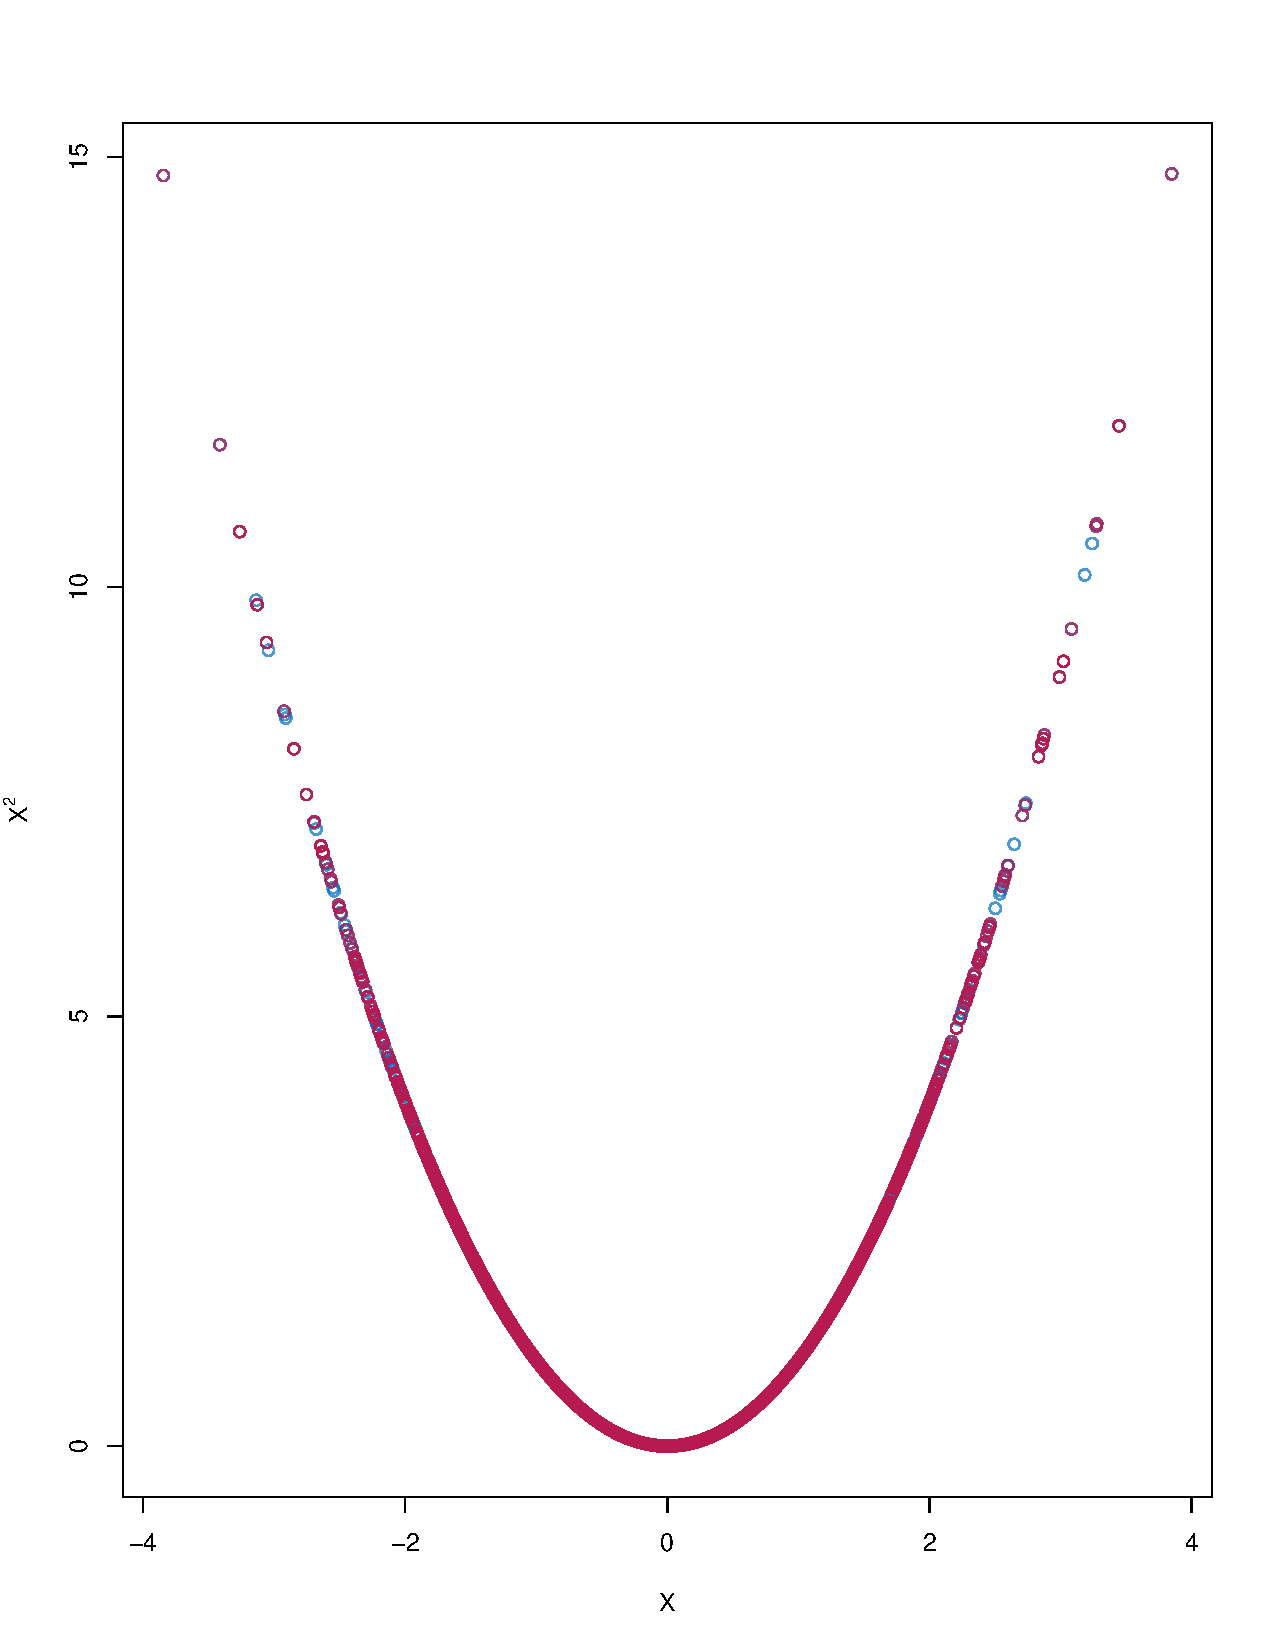
\includegraphics[width=\columnwidth]{plots/plot3.1.pdf}
		\caption{Predictive mean matching based on canonical regression analysis. Observed (blue) and imputed values (red) for $X$ and $X^2$.}
		\label{fig3_1}
	\end{figure}
	
	
	\subsection{Linear regression with interaction term}
	This section considers a linear regression substantive model, which includes two predictors and their interaction effect. 
	
	\subsubsection{Simulation conditions}
	The dependent variable $Y$ was generated according to the analysis model
	\begin{equation}
		\boldsymbol{Y} = \alpha+ \beta_1\boldsymbol{X_1} +  \beta_2\boldsymbol{X_2} + \beta_3\boldsymbol{X_1X_2} + \epsilon
	\end{equation}
	where $\alpha=0$, $\beta_1=1$, $\beta_2=1$, $\beta_3=1$, two predictors $\boldsymbol{X_1}$, $\boldsymbol{X_2}$ and error term $\epsilon$ were assumed as standard normal distributions. Under five types of missingness mechanisms: MCAR, MARleft, MARmid, MARtail, and MARright, the probability of jointly missing $X_1$ and $X_2$ was set to 0.4. There were no units with missing values on either $\boldsymbol{X_1}$ or $\boldsymbol{X_2}$. Missing values were amputed with the \texttt{ampute} function from the package \texttt{MICE} in \texttt{R}. For each simulation scenario, $n=5000$ units were generated and 1000 simulations were repeated.   
	
	\subsubsection{Estimation methods}
	We evaluated and compared the same methods as under section \ref{sec:3.4.1}, except the polynomial combination method. The model-based imputation method ensures a compatible imputation model by accommodating the designed model $\boldsymbol{Y} = \boldsymbol{X_1} + \boldsymbol{X_2} + \boldsymbol{X_1X_2} + \epsilon$. 
	
	
	\subsubsection{Results}
	\begin{table}[ht!]
		\centering
		\resizebox{\textwidth}{!}{
			\begin{tabular}{lcccccrl}
				\hline
				&\multicolumn{5}{c}{Missingness Mechanism} \\
				\cline{2-6}
				&MCAR	&MARleft	&MARmid		&MARtail	& MARright\\
				\hline
				\textit{Transform, then impute}	&&&&&\\
				Intercept ($\alpha$)				&0	&0.05	&-0.05 &0.06	&0.05\\
				Slope of $X_1$ ($\beta_1$)			&1(0.93)		&0.96(0.4)	&1(0.94)	&1.05(0.42)	&1.08(0.05)\\
				Slope of $X_2$ ($\beta_2$)		&1(0.94)		&0.96(0.4)	&1(0.96)	&1.05(0.38)	&1.09(0.02)\\
				Slope of $X_1X_2$($\beta_3$)    &1(0.94)        &0.96(0.53)    &0.95(0.25)    &1.06(0.31)    &1.09(0.02)\\
				Residual SD ($\sigma_\epsilon$) 	&1	&0.97	&1	&1.02	&1.04\\
				$R^2$						&0.75	&0.76	&0.75	&0.74	&0.73\\\\
				\textit{Impute, then transform}	&&&&&\\
				Intercept ($\alpha$)				&0	&-0.04	&-0.01	&0.01	&0.11\\
				Slope of $X_1$ ($\beta_1$)			&0.98(0.88)	&1.05(0.51)	&0.96(0.71)	&0.98(0.9)	&0.95(0.69)\\
				Slope of $X_2$ ($\beta_2$)		&0.98(0.88)	&1.05(0.48)	&0.96(0.73)	&0.98(0.92)	&0.95(0.69)\\
				Slope of $X_1X_2$($\beta_3$)    &0.64(0)  &0.64(0)  &0.7(0)  &0.54(0)  &0.61(0)\\
				Residual SD ($\sigma_\epsilon$) 	&1.25	&1.18	&1.22	&1.28	&1.37\\
				$R^2$						&0.61	&0.65	&0.63	&0.59	&0.53\\\\
				\textit{PMM-CRA}	&&&&&\\
				Intercept ($\alpha$)				&0	&0	&0	&0.01	&0.02\\
				Slope of $X_1$ ($\beta_1$)			&1(0.93)		&1(0.86)		&1(0.92)		&1.02(0.8)	&1.02(0.73)\\	
				Slope of $X_2$ ($\beta_2$)		&1(0.93)		&1(0.84)		&1(0.93)	&1.02(0.8)	&1.02(0.77)\\	
				Slope of $X_1X_2$($\beta_3$)     &1(0.94) &1.01(0.86)   &1(0.93) &1.02(0.71)  &1.03(0.68)\\
				Residual SD ($\sigma_\epsilon$) 	&1		&1.01		&1		&1.03	&1.03\\	
				$R^2$						&0.75	&0.74	&0.75	&0.74	&0.74\\\\
				\textit{SMC-FCS}	&&&&&\\
				Intercept ($\alpha$)				&0	&-0.01	&0	&0.01	&0.03\\
				Slope of $X_1$ ($\beta_1$)			&1(0.95)	&1.01(0.95)	&1(0.95)	&1(0.96)	&0.99(0.95)\\
				Slope of $X_2$ ($\beta_2$)		&0.99(0.94)	&0.99(0.93)	&1(0.97)	&1(0.96)	&0.99(0.96)\\
				Slope of $X_1X_2$($\beta_3$)    &1(0.95)  &1(0.96)  &1(0.95)   &1(0.97)  &1.01(0.93)\\
				Residual SD ($\sigma_\epsilon$) 	&1.02	&1.02	&1	&1.07	&1.06\\
				$R^2$						&0.74	&0.74	&0.75		&0.71	&0.72\\\hline
			\end{tabular}
		}
		\caption{Average parameter estimates for different imputation methods under five different missingness mechanisms over 1000 imputed datasets ($n=5000$) with 40\% missing data. The designed model is $Y = \alpha+ \beta_1X_1 +  \beta_2X_2 + \beta_3X_1X_2 + \epsilon$, where $\alpha=0$, $\beta_1=1$, $\beta_2=1$, $\beta_3=1$ and $\epsilon \sim N (0,1)$. The population coefficient of determination $R^2=.75$.}
		\label{tab3_3}
		
	\end{table}
	
	Table \ref{tab3_3} shows the estimates of $\alpha$, $\beta_1$, $\beta_2$, $\beta_3$, $\sigma_\epsilon$, $R^2$ and the coverage of the 95\% confidence intervals for $\beta_1$, $\beta_2$ and $\beta_3$. With MCAR, MARleft, and MARmid, MPMM was unbiased, and the CI coverage for regression weights was at the nominal level. While similar to the linear regression with quadratic term situation, with MARtail and MARright, MPMM yielded unbiased estimates but had relatively reduced confidence interval coverage. The reason is explained in section \ref{sec:3.4.1}. \emph{`Transform, then impute'} method did not preserve the relations even though it resulted in plausible inferences in cases of MCAR and MARmid. The imputations were not plausible. Moreover, with MARleft, MARtial, and MARright, \emph{`transform, then impute'} method gave severely biased estimates and extremely poor CI coverage. \emph{`Impute, then transform'} method generally yielded biased estimates, and the CI for coefficients $\beta_1$, $\beta_2$ and $\beta_3$ had lower than nominal coverage with all five types of missingness. SMC-FCS yielded unbiased estimates of regression weights and had correct CI coverage in all simulation scenarios. The only potential shortcoming of the model-based imputation method was that the estimates of $\sigma_\epsilon$ and $R^2$ showed slight deviations from true values with MARtail and MARright.  
	
	\subsection{Incomplete dataset with inequality restriction $\boldsymbol{X_1} + \boldsymbol{X_2} \geqq C$}
	\label{sec:3.4.3} 
	Multiple predictive mean matching is flexible to model relations among missing variables other than linear regression with polynomial terms or interaction terms. Lastly, we would evaluate the inequality restriction $\boldsymbol{X_1} + \boldsymbol{X_2} \geqq C$, which is relatively difficult for the model-based imputation approach to specify. One application of such inequality restriction would be the analysis of the academic performance of qualified students. For example, the sum score of mid-term and final exams should exceed a fixed value.  
	
	\subsubsection{Simulation conditions} 
	The data was generated from: 
	\begin{eqnarray*}
		\begin{pmatrix}\boldsymbol{X_{1}}\\
			\boldsymbol{X_{3}}
		\end{pmatrix} & \sim & \mathcal{N}\left[\left(\begin{array}{c}
			0\\
			1
		\end{array}\right),\left(\begin{array}{cc}
			4 & 3.2\\
			3.2 & 4
		\end{array}\right)\right],\\
	\end{eqnarray*}
	$\boldsymbol{X_2} = 3 - \boldsymbol{X_1} + \epsilon$, where $\epsilon$ followed a standard uniform distribution. The sum of $\boldsymbol{X_1} + \boldsymbol{X_2} \geqq 3$ was the restriction in the generated data. We simulated missingness such that rows in the block $(\boldsymbol{X_1, X_2,})$ were always either observed or completely missing. We considered 30\% joint missingness of $\boldsymbol{X_1}$ and $\boldsymbol{X_2}$. 2000 subjects were generated and 1000 simulations were performed for two missingness mechanisms : MCAR and MARright. We evaluated the mean of $X_1$ and $X_2$ and the coverage of nominal 95\% CIs. 
	
	\subsubsection{Estimation methods}
	We compared MPMM with PMM to illustrate the limited performance of univariate imputation approaches when there are relations connected to multiple missing variables. We did not apply joint modeling and univariate model-based imputation methods because it is hard to specify the designed inequality restriction.
	
	\subsubsection{Results}
	\begin{table}[ht!]
		\centering
		\resizebox{\textwidth}{!}{
			\begin{tabular}{ccc|cc|cc|cc}
				& \multicolumn{4}{c|}{MPMM}                                & \multicolumn{4}{c}{PMM}                                 \\\hline
				& \multicolumn{2}{c|}{MCAR} & \multicolumn{2}{c|}{MARright} & \multicolumn{2}{c|}{MCAR} & \multicolumn{2}{c}{MARright} \\\hline
				& MEAN      & COVERAGE     & MEAN        & COVERAGE       & MEAN      & COVERAGE     & MEAN        & COVERAGE       \\\hline
				$E(X_1)$ & 0         & 0.95         & 0.01        & 0.94           & 0         & 0.92         & -0.3        & 0              \\\hline
				$E(X_2)$ & 3.5       & 0.95         & 3.51        & 0.95           & 3.5       & 0.92         & 3.8         & 0             
			\end{tabular}
		}
		\caption{Average parameter estimates for MPMM and PMM under MCAR and MARright over 1000 imputed datasets ($n=2000$) with 30\% missing data. The designed model is introduced in section \ref{sec:3.4.3}. The true values of $E(X_1)$ and $E(X_2)$ are $0$ and $3.5$.}
		\label{tab3_4}
	\end{table}
	
	Table \ref{tab3_4} shows the mean estimates of $\boldsymbol{X_1}$ and $\boldsymbol{X_2}$ and coverage of the corresponding 95\% CIs. The true values for $E(\boldsymbol{X_1})$ and $E(\boldsymbol{X_2})$ are $0$ and $3.5$. MPMM yielded unbiased estimates with MCAR and MARright and had the correct CI coverage. However, PMM was unbiased with close to 95\% when the missingness mechanism is MCAR. It had considerable bias and extremely poor coverage with MARright. The reason is that the relations between $X_1$ and $X_2$ are not modeled \citep{Morris2014}.   
	
	\section{Conclusion}
	\label{sec:3.5}
	Predictive mean matching is an attractive method for missing data imputation. However, because of its univariate nature, PMM may not keep relations between variables with missing units. Our proposed modification of predictive mean matching, MPMM, is a multivariate extension of PMM that imputes a block of variables. We combine canonical regression analysis with predictive mean matching so that the models for donors selection are appropriate when there are restrictions involving more than one variable. MPMM could be valuable because it inherits the advantages of predictive mean matching and preserves relations between partially observed variables. Moreover, since predictive mean matching performs well in a wide range of simulation studies, so can the multivariate predictive mean matching.     
	
	We assess the performance of the multivariate predictive mean matching under three different substantive models with restrictions. In the first two simulation studies, MPMM provides unbiased estimates where the scientific model includes square terms and interaction terms under both MCAR and MAR missingness mechanisms. However, with MARtail and MARright, MPMM suffers the undercoverage issue because the density of the response indicator is heavy-tailed with our simulation setup. It makes units with large $Y$ almost unobserved and more missing than observed data in the tail region. The missingness mechanism is commonly moderate in practice, unlike MARtial and MARright in simulation studies. Overall, when no sub-regions of the sample space are sparsely observed, the multiple predictive mean matching analysis will provide unbiased estimates and correct CI coverage. 
	
	SMC-FCS yields better estimates and CI coverage of regression weights, but MPMM provides relatively accurate $\sigma_\epsilon$ and $R^2$. The comparison is not entirely fair because SMC-FCS, as used here, requires the correct substantive model for the data. In practice, we often do not know the model, and MPMM becomes attractive. MPMM is an easy-to-use method when increasing variables in the datasets or only the estimates are of interest. 
	
	The third simulation shows the appealing properties of MPMM. When relations of missing variables are challenging to model, MPMM becomes the most effective approach to imputation. We expect that MPMM could be applied to other relations not yet discussed in section \ref{sec:3.4}.    
	
	We limited our calculations and analyses to normal distributed $\boldsymbol{X}$. However, since Vink (2014) concluded that PMM yields plausible imputations with non-normal distributed predictors, we argue that distributions of predictors will not significantly impact the imputations. We focus on the simple case with one missing data pattern. One possible way to generalize MPMM to more complicated missing data patterns is proposed in the appendix. The general idea is to partition the cases into groups of identical missing data patterns in the block imputed with MPMM. We then perform the imputation in ascending order of the fraction of missing information, i.e., we first impute cases with relatively small missing data problems. Considering to impute partially observed covariates for linear regression with a quadratic term $Y = X + X^2$, we first impute cases with only missing value in $X^2$ by square the observed $X$. Then cases with only missing value in $X$ are imputed with one square root of $Y = X + X^2$. However, the selection of roots should be modeled with logistic regression. Finally, we impute cases with jointly missing $X$ and $X^2$ with MPMM. The comprehensive understanding of MPMM with multiple missing data patterns is an area for further research.         
	
	\section*{Appendix}
	The MPMM algorithm with multiple missing patterns:
	\begin{enumerate}
		\item Sort the rows of $\boldsymbol{Y}$ into $S$ missing data patterns $\boldsymbol{Y_{[s]}}, s=1,\cdots,S$.
		\item Initialize $\boldsymbol{Y_{mis}}$ by a reasonable starting value.
		\item Repeat for $T=1,\cdots,t$.
		\item Repeat for $S=1,\cdots,s$.
		\item Impute missing values by steps 1-8 of PMM-CRA algorithm proposed in section \ref{sec:3.2.3}.
		\item Repeat steps 1-5 \emph{m} times and save \emph{m} completed datasets.
	\end{enumerate} 
	
	

	



		\include{parts/part2}
		\chapter{How to relate potential outcomes: Estimating individual treatment effects under a given specified partial correlation} 
\label{chap4}
	\begin{abstract}
		In most medical research, the average treatment effect is used to evaluate a treatment's performance. However, precision medicine requires knowledge of individual treatment effects: What is the difference between a unit's measurement under treatment and control conditions? In most treatment effect studies, such answers are not possible, because the outcomes under both experimental conditions are not jointly observed. This makes the problem of causal inference a missing data problem. We propose to solve this problem by imputing the individual potential outcomes under a specified partial correlation (SPC), thereby allowing for heterogeneous treatment effects. We demonstrate in simulation that our proposed methodology yields valid inference for the marginal distribution of potential outcomes. We highlight that the posterior distribution of individual treatment effects varies with different specified partial correlations. This property can be used to study the sensitivity of optimal treatment outcomes under different correlation specifications. In a practical example on HIV-1 treatment data, we demonstrate that the proposed methodology generalises to real-world data. Imputing under the SPC therefore opens up a wealth of possibilities for studying heterogeneous treatment effects on incomplete data and the further adaptation of individual treatment effects.
	\end{abstract}
	
	\section{Introduction}
	\label{sec:4.1}
	Heterogeneity of treatment effects across individuals is a significant complication in precision treatment assignment to different persons. The difficulty of evaluating individual treatment effects (ITE) from the observed data is that only one of the potential outcomes is observed for each individual \citep{rubin1974estimating, hernan2010causal}. This fundamental problem of causal inference implies that causal inference is essentially a missing data problem \citep{rubin2005causal, ding2018causal}. Simply ignoring the missingness in the potential outcomes would only allow for average or homogeneous treatment effects. To allow for the estimation of unobserved heterogeneous treatment effects, we need to solve for the individual missing potential outcomes through multiple imputation. 
	
	Multiple imputation is a popular approach for analysing incomplete datasets but is not yet widely used in causal inference. In multiple imputation the missingness is solved before the data is analysed as if it were completely observed. Imputations for missing values are therein drawn from the corresponding posterior predictive distributions in parallel, resulting in multiple imputed datasets. Then, the statistical inference is obtained for each imputed dataset separately by complete-data analyses. Finally, the multiple analyses are aggregated into a single inference using Rubin's rules \citep[pp. 76]{RubinD1987}, which account for within, and across imputation uncertainty. Because multiple imputation imputes the individual potential outcomes, we can evaluate both the difference between outcomes and the individual treatment effects. 
	
	Studying individual treatment effects receives increasing attention. For example, \citet{lamont2018identification}, and \citet{westreich2015imputation} discussed the performance of multiple imputation for potential outcomes. \citet{lamont2018identification} applied multiple imputation to evaluate the effectiveness of various programs designed to prevent depression among sampled women and provide program recommendations for women out of the sample. However, \citet{lamont2018identification} and \citet{westreich2015imputation} fitted separate imputation models for potential outcomes based on observed covariates, thereby implicitly assuming conditional independence between potential outcomes. This conditional independence assumption is not always valid and cannot be verified from the observed data \citep{rassler2012statistical}. \citet{imbens2015causal} and \citet{gadbury2001evaluating} studied the sensitivity of the average treatment effect estimates under violations of the assumption of conditional independence between potential outcomes. They found that distributions of average causal effect under various partial correlations are different. An alternative imputation strategy fits a fully conditional model for the incomplete outcome. However, \citet{Buuren2018} demonstrated that without the specification of the partial correlation, the derived imputations for such models are unstable and can be implausible. 
	
	Specification of the partial correlation in applications of multiple imputation for potential outcomes has received little attention to date. We know that the partial correlation could be an arbitrary value between -1 and 1 in each imputed dataset. However, the imputations become poor when the partial correlation in the imputed dataset is negative \citep[Section 8.4.1]{Buuren2018}. We therefore assume that this correlation is non-negative. \citet{smink2016towards} proposed a data augmentation approach, where rows are added to the data that hold prior information for the partial correlation. This procedure is also outlined in \citep[Section 8.4.2]{Buuren2018}. In Smink's scenario, the imputations are guided by the specified correlation in the augmented cases, but the data does not hold any covariates. One could imagine that augmenting the data with a joint prior set becomes increasingly challenging when the number of covariates increases. 
	
	We propose a new hybrid imputation approach for imputing potential outcomes under a given partial correlation that allows for the collection of incomplete covariates. The procedure is hybrid in the sense that it combines properties from joint modeling imputation (the potential outcomes form a joint and are imputed as such) and fully conditional specification, wherein the covariates are imputed on a fully conditional variable-by-variable basis. In this manuscript we first outline the role of the partial correlation in causal inference, then give a brief overview of multiple imputation and introduce our new hybrid imputation approach. We evaluate the validity of the methodology in simulation and demonstrate the real-world applicability on a clinical trial aimed to evaluate the individual treatment effects of two different therapies on slowing the progression of HIV disease.	
	
	
	\section{The role of partial correlation}
	\label{sec:4.2}
	\subsection{Notation}
		Let ${Y(j), j = 1, \dots, p}$ denote one of $p$ incomplete variables and $Y(-j) = (Y(1), \dots, Y(j-1), Y(j+1), \dots, Y(p))$ denote the collection of the $p-1$ variables in $Y$ except $Y(j)$. In this paper, $Y(j)$ ususally represents the potential outcomes. Let $X = (X(1), \dots, X(k))$ be a set of $k$ completely observed variables. Let $\rho(Y(0), Y(1))$ be the correlation between two potential outcomes and $\rho_{Y(0), Y(1)\,|\ X}$ be the partial correlation between two potential outcomes. 
	\subsection{Setup}  
We focus on the case of a binary treatment $W_{i}$ and a continuous outcome $Y_{i}$ and assume the data come from a random sample of individuals, indexed by $i \in {1,\dots,N}$. Each individual $i$ has a nonzero probability to be assigned to both treatments, with $W_{i} = 1$ for the active treatment and $W_{i} = 0$ for the control treatment. The number of units under treatment and control are $N_{1}$ and $N_{0}$ respectively. We assume that the treatment assignment mechanism is unconfounded by the unobserved outcomes $Y_{mis}$, i.e., an ignorable assignment mechanism. We also assume that the potential outcomes for any individual are independent of the treatments assigned to others, which is known as the \emph{stable unit treatment value assumption} \citep{imbens2015causal}. Here the ignorable or unconfounded assignment mechanism implies that $P(W|Y(0), Y(1), X) = P(W|Y_{obs}, X)$, where X are observed covariates not influenced by treatment assignment. The individual treatment effect is defined as $\tau_{i} = Y_{i}(1) - Y_{i}(0)$. We assume a joint distribution for the potential outcomes $Y_{1}$ and $Y_{0}$ and that the correlation between the potential outcomes $\rho(Y_{1}, Y_{0})$ can be quantified by one or more parameters. The imputation models for missing outcomes $Y(1)$ and $Y(0)$ are: 
\begin{align}
	\dot{Y}(1) &\sim P(Y^{mis}(1)|Y^{obs}(1), Y(0), X, \dot{\phi}_{1})\\
	\dot{Y}(0) &\sim P(Y^{mis}(0)|Y^{obs}(0), Y(1), X, \dot{\phi}_{0}),
\end{align}
where parameters of the imputation model $\dot{\phi}_{1}$ and $\dot{\phi}_{0}$ are draws from their respective posterior distribution.
	\subsection{Partial correlation between potential outcomes}
	The necessity of specifying the partial correlation in the process of multiple imputation has been discussed hereinbefore. This section would further illustrate the causality meaning of the partial correlation. We decompose the individual treatment effect $\tau_{i} \in T, i = 1, \dots, N$ via
	\begin{equation}
		\begin{array}{lr}
			\tau_{i} = Y_{i}(1) - Y_{i}(0) = X_{i}^{\mathsf{T}}\beta + \varepsilon_{i},
		\end{array}
	\end{equation}
	where $X_{i}$ are observed pre-treatment covariates for individual $i$. Under random treatment assignment, the regression weight $\beta$ could be the ordinary least-square (OLS) estimation of $\tau_{i}$ on $X_{i}$. The quantity $X_{i}^{\mathsf{T}}\beta$ is known as systematic treatment effect variation and the residual $\varepsilon_{i}$ is the idiosyncratic treatment effect variation not explained by $X_{i}$ \citep{ding2019decomposing, heckman1997making, djebbari2008heterogeneous}. The idiosyncratic variation accounts for treatment effect variation not attributable to differences in observed covariates. Based on the formula of OLS estimation, the coefficient 
	\begin{equation}
		\begin{array}{cl}
			\beta &= (X^{\mathsf{T}}X)^{-1}X^{\mathsf{T}}T \\
			&= (X^{\mathsf{T}}X)^{-1}X^{\mathsf{T}}Y(1) - (X^{\mathsf{T}}X)^{-1}X^{\mathsf{T}}Y(0) \\
			&= \beta_{1} -\beta_{0},
		\end{array}
	\end{equation}
	where $\beta_{1}$ and $\beta_{0}$ are the corresponding regression weights of the potential outcomes $Y_{1}$ and $Y_{0}$ on the observed covariates $X$. Similarly, the idiosyncratic treatment effect variation $\varepsilon_{i}$
	\begin{equation}
		\begin{array}{cl}
			\varepsilon_{i} &= \tau_{i} - X_{i}^{\mathsf{T}}\beta\\
			&= (Y_{i}(1)  - X_{i}^{\mathsf{T}}\beta_{1}) - (Y_{i}(0) - X_{i}^{\mathsf{T}}\beta_{0})\\
			&= \varepsilon_{i}(1) -\varepsilon_{i}(0),
		\end{array}
	\end{equation} 
	where $\varepsilon(1)$ and $\varepsilon(0)$ are the residuals from the regression of the potential outcomes $Y_{1}$ and $Y_{0}$ on the observed covariates $X$. Applying the theory of variance decomposition for linear regression, we could decompose the variance of individual treatment effect into two components:
	\begin{equation}
		\text{Var}(\tau_{i}) = \text{Var}(X_{i}^{\mathsf{T}}\beta) + \text{Var}(\varepsilon_{i}). 
	\end{equation}
	Based on the idiosyncratic treatment effect variation formula (5), the idiosyncratic components of individual treatment variance becomes
	\begin{equation}
		\begin{array}{cl}
			\text{Var}(\varepsilon_{i}) &= \text{Var}[\varepsilon_{i}(1) -\varepsilon_{i}(0)]\\ 
			&= \text{Var}[\varepsilon_{i}(1)] + \text{Var}[\varepsilon_{i}(0)] - 2\text{Cov}[\varepsilon_{i}(1), \varepsilon_{i}(0)], 
		\end{array}
	\end{equation} 
	which demonstrate that partial correlation $\rho_{Y(0)Y(1)\,|\ X}$ between the potential outcomes does impact the idiosyncratic variation, which is unidentifiable from the observed data. 
	
	Although the relation between potential outcomes cannot be determined solely from the observed data, there are still some approaches to identifying the partial correlation, such as the model-based approach, the experiment-based approach, and sensitivity analysis. The model-based approach explicitly models the relationship between the idiosyncratic variation and the assignment mechanisms such that the partial correlation would be close or equal to zero \citep{heckman2005scientific}. Economists usually deal with ex-post causal inference. The agents select the treatment according to their ex-ante evaluation. In this case, economists could infer the information only available to agents from the assignment mechanism.  For instance, \citet{heckman2010effects} investigated the causal effect of educational decisions on the labour market and health outcomes. He modelled latent cognitive and social-emotional endowments and included these latent variables into the outcome equations. As indicated earlier, the partial correlation between potential outcomes is the only unknown parameter in the formula of idiosyncratic variation. Therefore, the model for idiosyncratic variation could be tailored to the model for the partial correlation between potential outcomes. Generally, the model-based approach attempts to figure out latent variables affecting the partial correlation between potential outcomes. 
	
	The experiment-based approach intends to design sophisticated experiments to collect additional data where analysts could evaluate the partial correlation between potential outcomes. For instance, the experiment-based approach collects repeated measurements under more than one treatment level for the same individual from which some relevant information about the partial correlation between potential outcomes is available. The experiment designed for repeat measurements is known as N-1 trails \citep{shamseer2015consort, araujo2016understanding}. Researchers could also design an auxiliary treatment ($W_{i} = 2$) and assign the extensive treatment to all individuals in the sample. Then the individual treatment effect $Y_{i}(1) - Y_{i}(0)$ can be evaluated by $[Y_{i}(2) - Y_{i}(0) - (Y_{i}(2) - Y_{i}(1))]$. 
	
	Both model-based and experiment-based approaches search for extra information to determine the partial correlation between potential outcomes. If such additional information is not available, the alternative is sensitivity analysis. After imputing the missing potential outcomes, one could evaluate individual treatment effects with various valid partial correlations and study the effect of partial correlations on the conclusions \citep{gadbury2001evaluating}.  
	
	\section{Multiple imputation of multivariate incomplete variables}
	\label{sec:4.3}
	Datasets used for evaluating individual treatment effects by multiple imputation often have incomplete covariates and potential outcomes. We impute potential outcomes with joint modeling (JM) and covariates with fully conditional specification (FCS). Usually, one framework is used to generate all imputations, but \citet{Buuren2018} highlighted that a blocked approach could be adopted to accommodate for hybrid versions of JM within FCS. We will now briefly introduce joint modelling, fully conditional specification and so-called hybrid imputation. 
	\subsection{Joint modeling imputation (JM)}
	Joint modeling imputation assumes a model $p(Y^{mis}, Y^{obs}\,|\,\theta)$ for the complete data and a prior distribution $p(\theta)$ for the parameter $\theta$. Joint modelling partitions the observed data into groups based on the missing pattern and imputes the missing data within each missing pattern according to corresponding predictive distribution. Under the assumption of ignorability, the parameters of the predictive distribution for different missing patterns are generated from the posterior joint distribution. \citet{schafer1997analysis} proposed joint modelling methods for multivariate normal data, categorical data and mixed normal-categorical data. The joint modelling approach has solid theoretical properties (i.e., compatibility between the imputation and substantive models) while it lacks the flexibility of model specification.
	
	\subsection{Fully Conditional Specification (FCS)}
	In Fully Conditional Specification, we specify the distribution for each partially observed variable conditional on all other variables $P(Y(j)|Y(-j), X, \theta_{j})$ and impute each missing variable iteratively. The FCS starts with naive imputations such as a random draw from the observed values. The \emph{t}th iteration for the incomplete variable \emph{$Y(j)$} consists of the following draws:
	\begin{align*}
		&\theta_{j}^{t} \sim f(\theta_{j})f(Y^{obs}(j)|Y^{t-1}(-j), X, \theta_{j})\\
		&Y^{mis(t)}(j) \sim f(Y^{mis}(j)|Y^{t}(-j), X, \theta_{j}^{t}),
	\end{align*}
	where $f(\theta_{j})$ is generally specified as a noninformative prior. After a sufficient number of iteration, typically with 5 to 10 iterations \citep{Buuren2018}, the stationary distribution is achieved. The final iteration generates a single imputed dataset and the multiple imputations are created by applying FCS in parallel \emph{m} times. Since FCS provides tremendous flexibility in specifying imputation models for multivariate partially observed data, FCS is now a widely accepted and popular MI approach \citep{van2007multiple}. Even while, FCS lacks a satisfactory theory and has a potential risk in incompatibility. 
	
	\subsection{Block imputation}
	Block imputation combines the flexibility of FCS with the attractive theoretical properties of JM. A block consists of one or more variables. If the block has multiple variables, then we use multivariate imputation methods to impute those variables jointly. A simple example would be multiple imputation of missing variables with quadratic effects $Y = \alpha + \beta_{1}X + \beta_{2}X^2 + \varepsilon$. In such a case, grouping the missing variable $X$ and its corresponding square term $X^2$ within one block is of benefit to preserve the quadratic relationship \citep{vink2019}. The joint modelling approach is the special case where all variables form one block, while the FCS approach treats each variable as a separate block. 
	
	When the imputation model of one variable is potentially incompatible, or its theoretical properties are not fully studied (i.e., whether the imputations based on the FCS correspond to drawing from a joint distribution), block imputation would merge that variable with other variables and apply the joint modeling imputation approach to that block. On the other hand, when the joint distribution of several missing variables is ambiguous, block imputation could use the FCS approach to impute each variable. In general, the apparent advantage of block imputation is the flexibility of model specification. However, block methods are hardly known or studied. While available in the \texttt{mice} software, the properties of block imputation have yet to be studied.  
	
	\section{Specified partial correlation imputation}
	\label{sec:4.4}
	\begin{figure}[ht!]
		\centering
		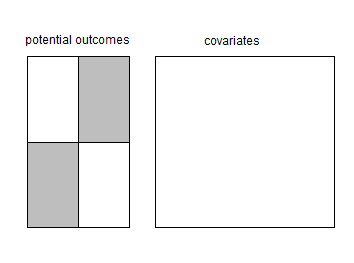
\includegraphics[width=1.0\linewidth,height=0.5\textheight]{plots/potentialoutcome} 
		\caption{Missingness mechanism of potential outcomes. The write represents observed value and the grey represents missing value. Without loss of generality, we assume covariates are completely observed.}
		\label{fig4_1}
	\end{figure}
	
	In this section we detail how blocked imputation can be used to impute missing outcomes with a given partial correlation between potential outcomes. We term the algorithm the imputation algorithm with specified partial correlation (SPC). Since the missing pattern of potential outcomes is somehow restrictive (see Figure \ref{fig4_1}) that is, no cases with completely observed potential outcomes, the imputation procedure follows three steps: 
	
	\begin{enumerate}
		\item Estimating the marginal distribution of potential outcomes conditioning on pre-treatment variables. 
		\item Derive the multivariate density of potential outcomes by combining the marginal distribution of potential outcomes and the specified correlation between potential outcomes. 
		\item Impute the missing outcomes with the corresponding submodel obtained from the multivariate distribution. 
	\end{enumerate}	
	
	Based on Rubin causal model \citep[Ch 8]{imbens2015causal}, it is plausible to assume a multivariate normal distribution for continuous potential outcomes. However, it is usually not valid to assume a joint distribution for the incomplete dataset. Applying fully conditional specification to impute covariates allows flexibility of imputation model specification. It is noticeable that SPC could also predict the posterior distribution of the individual treatment effect for units not in the experiment.  
	
	Our approach shares some similarities with statistical matching discussed by \citep{moriarity2003note}. For example, suppose there are two sample files, A and B. File A collects variables $X$ and $Y$ and file B collects variables $X$ and $Z$. The purpose of statistical matching is to combine two files, A and B, into one file containing variables $X$, $Y$ and $Z$. \citet{rubin1986statistical} proposed a procedure of statistical matching with three steps: regression step, matching step and concatenation step. In the regression step, Rubin specified the correlation between variable $X$ and $Y$ to derive the joint distribution of ($X$, $Y$, $Z$) in two sample files. We develop this idea to evaluate the individual treatment effects and extend to multiple treatments condition.  
	%In practice, the potential outcomes sometimes should be tailored to more or less normal distribution.  
	
	Without loss of generality, let us assume that potential outcomes follow a multivariate normal distribution. We specify Bayesian linear models for two potential outcomes based on observed covariates. 
	\begin{align}
		Y(0) = \beta_{0}X + \varepsilon_{0}, \varepsilon_{0} \sim \mathcal{N}(0, \sigma_{0}^2)\\
		Y(1) = \beta_{1}X + \varepsilon_{1}, \varepsilon_{1} \sim \mathcal{N}(0, \sigma_{1}^2).
	\end{align}
	Bayesian sampling draws $\beta_{0}^{*}$, $\beta_{1}^{*}$, $\sigma_{0}^{*2}$, $\sigma_{1}^{*2}$ from their respective posterior distribution. The Jeffrey's prior used and hence, the posterior distributions of $\sigma_{0}^{*2}$ and $\sigma_{1}^{*2}$ would be inverse $\chi^2$ distribution:
	\begin{align}
		\sigma_{0}^{*2} \sim \sum_{i = 1}^{N_{0}}(Y_i(0) - \hat{\beta}_{0}X_{i})^2\chi_{N_{0} - k}^{-2}\\
		\sigma_{1}^{*2} \sim \sum_{i = 1}^{N_{1}}(Y_i(1) - \hat{\beta}_{1}X_{i})^2\chi_{N_{1} - k}^{-2},
	\end{align}
	where $\hat{\beta}_{0} = (X_{0}'X_{0})^{-1}X_{0}'Y(0)$, $\hat{\beta}_{1} = (X_{1}'X_{1})^{-1}X_{1}'Y(1)$ and \emph{k} is the number of covariates. The conditional distributions of  $\beta_{0}^{*}$ and $\beta_{1}^{*}$ are multivariate normal:
	\begin{align}
		\beta_{0}^{*} | \sigma_{0}^{*2} \sim \mathcal{N}(\hat{\beta}_{0}, \sigma_{0}^{*2}((X_{0}'X_{0})^{-1}))\\
		\beta_{1}^{*} | \sigma_{1}^{*2} \sim \mathcal{N}(\hat{\beta}_{1}, \sigma_{1}^{*2}((X_{1}'X_{1})^{-1})).
	\end{align}
	Since there is no information relevant to the partial correlation between potential outcomes in the observed data, the posterior distribution of the partial correlation $\rho_{Y(0)Y(1)|X}$ equals the prior distribution specified by the user, who can select several numbers in the interval [$-1$, $1$] to investigate the sensitivity to $\rho_{Y(0)Y(1)|X}$. 
	Finally, combined the marginal distribution of $Y(0)$ and $Y(1)$ with the specification of $\rho_{Y(0)Y(1)|X}$, the joint distribution of $Y^{mis}(0)$ and $Y^{mis}(1)$ is:
	\begin{eqnarray}
		\left[\begin{array}{c}
			Y^{mis}(0)\\
			Y^{mis}(1)
		\end{array}\right] & \sim & \mathcal{N}\left[\left(\begin{array}{c}
			\beta^{*}_{0}x\\
			\beta^{*}_{1}x
		\end{array}\right),\left(\begin{array}{cc}
			\sigma^{*2}_{0} & \rho_{Y(0)Y(1)|X}\sigma^{*}_{0}\sigma^{*}_{1}\\
			\rho_{Y(0)Y(1)|X}\sigma^{*}_{0}\sigma^{*}_{1} & \sigma^{*2}_{1}
		\end{array}\right)\right],
	\end{eqnarray}
	and the distributions of $Y^{mis}(0)$ and $Y^{mis}(1)$ are:
	\begin{align}
		Y^{mis}(0) \sim \mathcal{N} (\beta^{*}_{0}x + (Y(1) - \beta^{*}_{1}x)\rho_{Y(0)Y(1)|X}\sigma_{0} / \sigma_{1}, (1 - \rho_{Y(0)Y(1)|X}^2)\sigma^{*2}_{0})\\
		Y^{mis}(1) \sim \mathcal{N} (\beta^{*}_{1}x + (Y(0) - \beta^{*}_{0}x)\rho_{Y(0)Y(1)|X}\sigma_{1} / \sigma_{0}, (1 - \rho_{Y(0)Y(1)|X}^2)\sigma^{*2}_{1}).
	\end{align}
	Comparing equations (15) and (16) to equations (8) and (9), it is evident that inclusion of the observed outcome may change the location of missing outcomes shifts slightly and the uncertainty is reduced when imputing missing outcomes under the specified correlation between potential outcomes. For the prediction of units out of trials, the reasonable values for outcomes under two treatments could be drawn from the joint distribution (14). 
	
	When generalizing to the multiple treatments condition $W = 0, 1,\dots,w$, the marginal posterior distribution for potential outcomes would be:
	\begin{align*}
		Y(0)^{*} &= \beta_{0}^{*}X + \varepsilon_{0}^{*}, \varepsilon_{0}^{*} \sim \mathcal{N}(0, \sigma_{0}^{*2})\\
		Y(1)^{*} &= \beta_{1}^{*}X + \varepsilon_{1}^{*}, \varepsilon_{1}^{*} \sim \mathcal{N}(0, \sigma_{1}^{*2})\\
		&\dots\\
		Y(w)^{*} &= \beta_{w}^{*}X + \varepsilon_{w}^{*}, \varepsilon_{w}^{*} \sim \mathcal{N}(0, \sigma_{w}^{*2}),
	\end{align*}
	where the values of $\beta_{0}^{*}$, $\beta_{1}^{*}$, \dots, $\beta_{w}^{*}$, $\sigma_{0}^{*2}$, $\sigma_{1}^{*2}$, \dots, $\sigma_{w}^{*2}$  draw from their respective Bayesian posterior distribution.
	If $\sigma_{0}^{*2}, \dots, \sigma_{w}^{*2}$ are unrestricted, with pairwise specification of partial correlation between potential outcomes, the joint distribution of $Y^{mis}(0)$, $Y^{mis}(1)$, \dots, $Y^{mis}(w)$ is:
	\begin{eqnarray}
		\left[\begin{array}{c}
			Y^{mis}(0)\\
			Y^{mis}(1)\\
			\dots\\
			Y^{mis}(w).
		\end{array}\right] & \sim & \mathcal{N}(\mathcal{M}, \Sigma),
	\end{eqnarray}
	where  $\mathcal{M} = (\beta^{*}_{0}x, \beta^{*}_{1}x, \dots, \beta^{*}_{w}x)^{\mathsf{T}}$. The covariance matrix $\Sigma$ must be positive semi-definite:
	\begin{eqnarray}
		\begin{array}{c}
			\Sigma
		\end{array} = \left(\begin{array}{cccc}
			\sigma^{*2}_{0} & \rho_{Y(0)Y(1)|X}\sigma^{*}_{0}\sigma^{*}_{1} & \dots & \rho_{Y(0)Y(w)|X}\sigma^{*}_{0}\sigma^{*}_{w}\\
			\rho_{Y(1)Y(0)|X}\sigma^{*}_{1}\sigma^{*}_{0} & \sigma^{*2}_{1} & \dots & \rho_{Y(1)Y(w)|X}\sigma^{*}_{1}\sigma^{*}_{w}\\
			\vdots & \vdots & \ddots & \vdots\\
			\rho_{Y(w)Y(0)|X}\sigma^{*}_{w}\sigma^{*}_{0} & \rho_{Y(w)Y(1)|X}\sigma^{*}_{w}\sigma^{*}_{1} & \dots & \sigma^{*2}_{w}
		\end{array}\right).
	\end{eqnarray} 
	Draws of missing outcomes for units under different treatments could be derived from the joint distribution based on the property of conditional distribution for the multivariate normal distribution. For instance, with units under control treatment $W = 0$, the distribution of missing outcomes $Y^{mis}(-0) = (Y^{mis}(1), \dots, Y^{mis}(w))$ would be $Y^{mis}(-0) \sim \mathcal{N} ((\beta^{*}_{1}x, \dots, \beta^{*}_{w}x)^{\mathsf{T}} + \Sigma_{0-0}\Sigma_{-0-0}^{-1}(Y_0 - \beta^{*}_{0}x), \Sigma_{00} - \Sigma_{0-0}\Sigma_{-0-0}^{-1}\Sigma_{-00})$, where
	\begin{eqnarray}
		\left[\begin{array}{cc}
			\Sigma_{00} & \Sigma_{0-0}\\
			\Sigma_{-00} & \Sigma_{-0-0}
		\end{array}\right],
	\end{eqnarray}
	is the partition of $\Sigma$: $\Sigma_{00} = \sigma^{*2}_{0}$, $\Sigma_{0-0} = \Sigma_{-00}^{\mathsf{T}} = (\rho_{Y(0)Y(1)|X}\sigma^{*}_{0}\sigma^{*}_{1}, \dots, \rho_{Y(0)Y(w)|X}\sigma^{*}_{0}\sigma^{*}_{w})$ and 
	\begin{eqnarray}
		\begin{array}{c}
			\Sigma_{-0-0}
		\end{array} = \left(\begin{array}{cccc}
			\sigma^{*2}_{1} & \dots & \rho_{Y(1)Y(w)|X}\sigma^{*}_{1}\sigma^{*}_{w}\\
			\vdots & \vdots & \ddots & \vdots\\
			\rho_{Y(w)Y(1)|X}\sigma^{*}_{w}\sigma^{*}_{1} & \dots & \sigma^{*2}_{w}
		\end{array}\right).
	\end{eqnarray} 
	One could use the sweep operator for rapid calculation of the parameters for imputation models of missing outcomes \citep{goodnight1979tutorial}. 
	
	\section{Simulation study}
	\label{sec:4.5}
	We evaluate the performance of SPC at both the individual level (i.e. the individual treatment effect) and the aggregate level (i.e. the average treatment effect). For individual causal inference, we study the mean and mean absolute differences between the `true' and imputed individual treatment effects, together with posterior distributions of individual treatment effects. For average causal inference, we analyse biases and confidence interval coverages of the estimated parameters in the distribution of the potential outcomes. We perform a sensitivity analysis to the multiple imputation approach with three different values for the partial correlation between potential outcomes: $\rho = 0, 0.73 $ or $0.99$, which correspond to, respectively, a conditional independent correlation assumption, the correct partial correlation and a constant treatment effect condition. 
	
	We compare the performance of SPC to the targeted learning approach by \citet{van2011targeted}. Targeted learning is an alternative for estimating individual treatment effects. The idea is to estimate the data-generating distribution $P_{0}$ and then update the initial estimation to make an optimal bias-variance tradeoff for the scientific interest $\Psi(P_{0})$. To estimate individual treatment effects, we define the average treatment effect as the scientific interest:
	\begin{equation}
		\Psi(P_{0}) = E[E(Y_{i}(1)\,|\,X) - E(Y_{i}(0)\,|\,X)].
	\end{equation} 
	The targeted learning consists of three steps of analysis: 1) definition of the data-generating model and the scientific interest $\Psi(P_{0})$, 2) super learning for initial prediction of $\Psi(P_{0})$ and 3) targeted maximum likelihood estimation for $\Psi(P_{0})$ \citep{van2011targeted}. Specifically, before estimation, it is necessary to define a set of possible probability distributions of observed data and identify a collection of causal assumptions (i.e., the ignorable assignment mechanism and the stable unit treatment value assumption) to the identification of the correct model. With the definition of the model, one could apply the super learner to derive an initial estimation for the distribution of potential outcomes $\hat{P}_0$. The super learner first selects a library of candidate algorithms and a risk function and then applies the validation set approach to calculate the average risk for each algorithm. The optimal algorithm with the smallest average risk is used to produce the initial predicted distribution of potential outcomes. The candidate algorithms could be parametric(i.e., general linear model), non-parametric (i.e., random forest), or even a weighted combination of statistical algorithms. 
	
	After the initial estimation of predicted potential outcomes, one could define the targeted maximum likelihood estimation (TMLE) for scientific interest $\Psi(P_{0})$. The TMLE step reduces the bias in the estimation of $\Psi(P_{0})$ if the initial estimation $\Psi(\hat{P}_0)$ is inconsistent. This is accomplished by exploiting information in the treatment assignment mechanisms to adjust the initial estimations. Generally, the adjustment is an iterative procedure. However, when the scientific interest is the average treatment effect, convergence is achieved in one step. More details are provided in \citet{gruber2011tmle}.    
	
	While targeted learning is a machine learning approach aimed at estimating the average treatment effect, it involves calculating the missing potential outcomes and can therefore also be used to identify individual treatment effects. However, unlike SPC, the targeted learning fits the distribution of the missing outcome only based on the covariates, which assumes conditional independence between potential outcomes. In the simulation study, we aim to show the relevance of specifying the correlation between potential outcomes when specifying the analysis model of potential outcomes.              
	\subsection{Simulation conditions}
	\label{sec:4.5.1}
	We design the two potential outcomes $Y(0)$ and $Y(1)$ as well as one baseline covariate $X$. The data is generated with a multivariate normal distribution:
	\begin{eqnarray*}
		\begin{pmatrix}Y_{0}\\
			Y_{1}\\
			X
		\end{pmatrix} & \sim & \mathcal{N}\left[\left(\begin{array}{c}
			0\\
			1\\
			2
		\end{array}\right),\left(\begin{array}{ccc}
			1 & 0.8 & 0.5\\
			0.8 & 1 & 0.5\\
			0.5 & 0.5 & 1
		\end{array}\right)\right]\\
	\end{eqnarray*}
	Because the marginal correlation between potential outcomes is 0.8, the corresponding partial correlation is 0.73. 
	\begin{equation}
		\begin{array}{cl}
			\rho_{y_{0}y_{1}|x} &= \frac{\rho_{y_{0}y_{1}} - \rho_{y_{0}x}\rho_{y_{1}x}}{\sqrt{1 - \rho_{y_{0}x}^2}\sqrt{1 - \rho_{y_{1}x}^2}} \\
			&= \frac{0.8 - 0.25}{0.75}\\
			&\approx 0.73,
		\end{array}
	\end{equation}
	A total of $N = 5000$ independent and identically distributed cases are generated. The first 2500 cases have only information for $Y_0$ and the remaining cases have only information on $Y_1$. One thousand repetitions of the simulation are produced for average causal inference. While, for individual causal inference, we derive the posterior distributions of imputed outcomes from twenty imputed datasets. For reasons of brevity, we only include one pre-treatment covariate. However, it is straightforward to extend the methodology to situations with more covariates and even mixtures of continuous and categorical predictors.
	    
	
	\subsection{Results}
	\label{sec:4.5.2}
	\subsubsection{Individual causal inference}
	We define bias as the mean difference between \emph{true} and estimated values over twenty imputed datasets. Figure \ref{fig4_2} shows the distribution of the bias for all four strategies, and the corresponding location and scale are displayed in Table \ref{tab4_1}.  
\begin{figure}[ht!]
	\begin{center}
		\resizebox{\textwidth}{!}{
			\subfigure[BLI-SPC $\rho_{partial} = 0$]{
				\label{boxplot:a}
				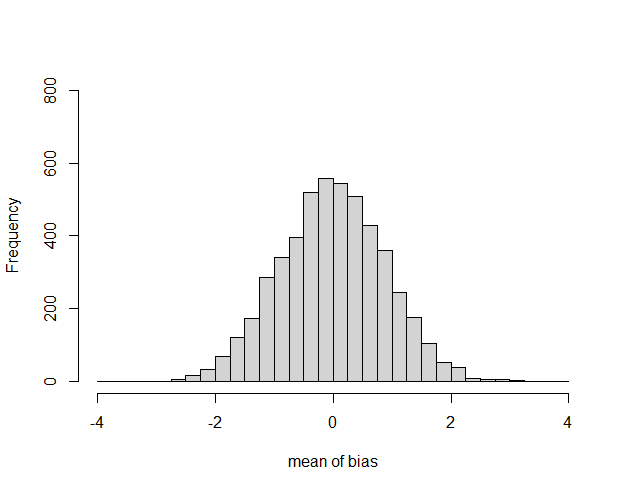
\includegraphics[scale=.5]{plots/plot4.1}
			}
			\subfigure[BLI-SPC $\rho_{partial} = 0.73$]{
				\label{boxplot:b}
				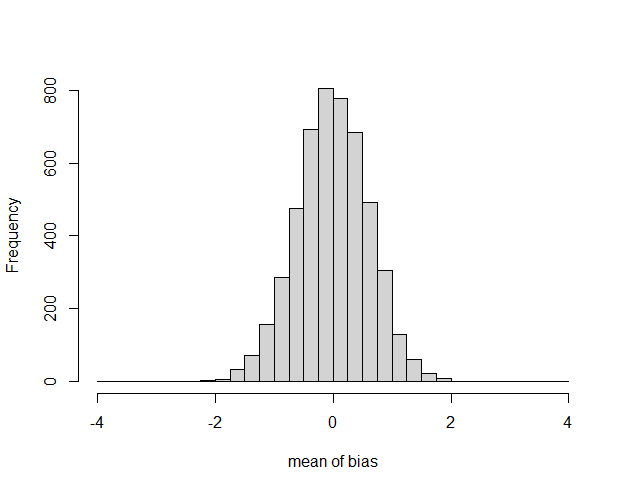
\includegraphics[scale=.5]{plots/plot4.2}
			}
		}\\ 	
		\resizebox{\textwidth}{!}{
			\subfigure[BLI-SPC $\rho_{partial} = 0.99$]{
				\label{boxplot:c}
				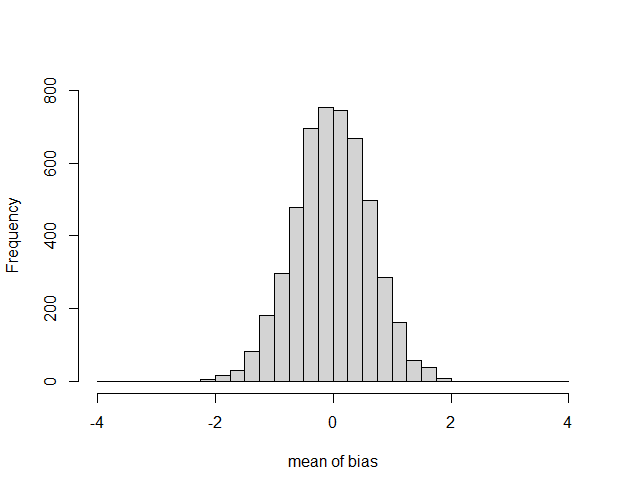
\includegraphics[scale=.5]{plots/plot4.3}
			}
			\subfigure[The targeted learning]{
				\label{boxplot:d}
				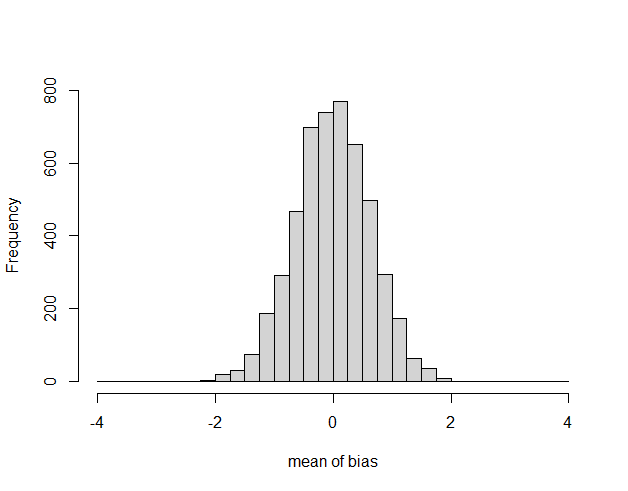
\includegraphics[scale=.5]{plots/plot4.4}
			}
		}
	\end{center}
	\caption{Histrogram plots of the bias of estimate the individual treatment effects for all four strategies.}
	\label{fig4_2}
\end{figure}

\begin{table}[ht!]
	\centering
	\begin{tabular}{c|cc}
		$\rho_{Y(0)Y(1)\,|\ X}$                       & Mean   & Variance \\
		\hline                              
		BLI-SPC $\rho_{partial} = 0$       & -0.012     & 0.791 \\
		BLI-SPC $\rho_{partial} = 0.73$    & -0.007     & 0.363 \\
		BLI-SPC $\rho_{partial} = 0.99$    & -0.013     & 0.398 \\
		The targeted learning         & -0.006 & 0.401 
	\end{tabular}
	\caption{The location and the scale for the bias of estimate the individual treatment effects for all four strategies.}
	\label{tab4_1}
\end{table} 

\begin{figure}[ht!]
	\centering
	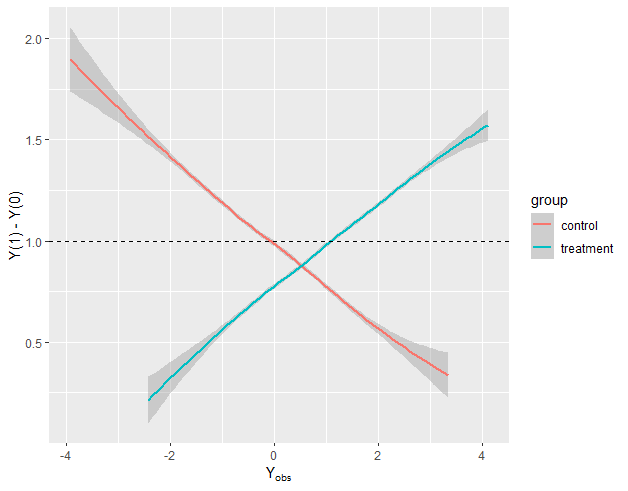
\includegraphics[width=1.0\linewidth,height=0.5\textheight]{plots/plot4.5} 
	\caption{The plot shows mean individual treatment effects $(Y(1) - Y(0))$ in both treatment and control group when partial correlation is defined as $0.73$. The oucome $Y(0)$ is observed in the control group and the oucome $Y(1)$ is observed in the treatment group. The dashed line represents the average treatment effect.}
	\label{fig4_3}
\end{figure}
	Overall, SPC with three different partial correlations and the targeted learning all yield unbiased estimates of the average treatment effect. However, in terms of the scale, The SPC with the \emph{correct} partial correlation has a minor variance. The closer the specified partial correlation is to the partial correlation in the \emph{true} data generating model, the smaller bias and variance can be expected. Although it is difficult to produce accurate estimates of the individual treatment effect for units at the tail in Fig \ref{fig4_3}, we still have a large proportion of the estimated individual treatment effect with negligible biases. Since the variance of the bias equals the partial variance of the potential outcomes, we could include more explanatory variables to increase the accuracy of the imputation of missing outcomes and hence the prediction of individual treatment effect. On the other hand, when the specified partial correlation deviates from the \emph{true} value, more variance would appear because of the differences between the \emph{true} distribution and the estimated distribution for each missing outcome. 
	
	
	\begin{figure}[ht!]
		\begin{center}
			\resizebox{\textwidth}{!}{
				\subfigure[BLI-SPC $\rho_{partial} = 0$]{
					\label{boxplot:e}
					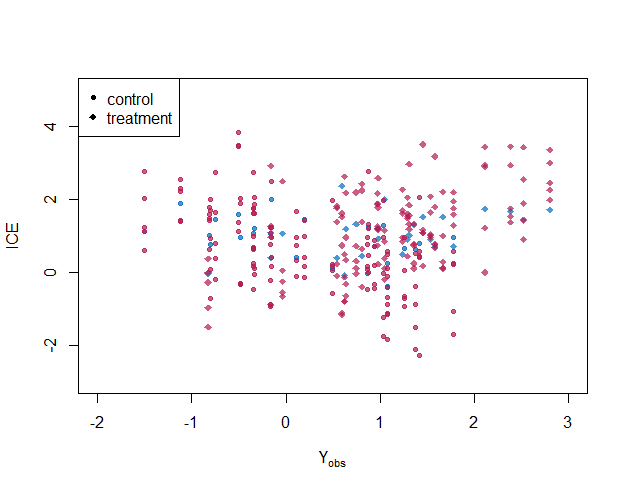
\includegraphics[scale=.5]{plots/plot4.6}
				}
				\subfigure[BLI-SPC $\rho_{partial} = 0.73$]{
					\label{boxplot:f}
					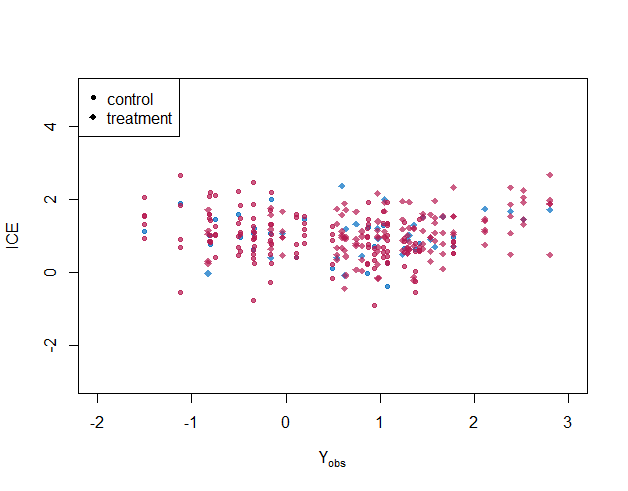
\includegraphics[scale=.5]{plots/plot4.7}
				}
			}\\ 	
			\resizebox{\textwidth}{!}{
				\subfigure[BLI-SPC $\rho_{partial} = 0.99$]{
					\label{boxplot:g}
					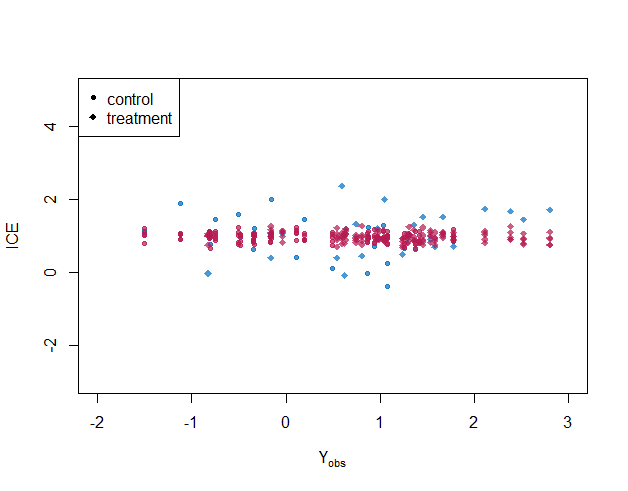
\includegraphics[scale=.5]{plots/plot4.8}
				}
				\subfigure[The targeted learning]{
					\label{boxplot:h}
					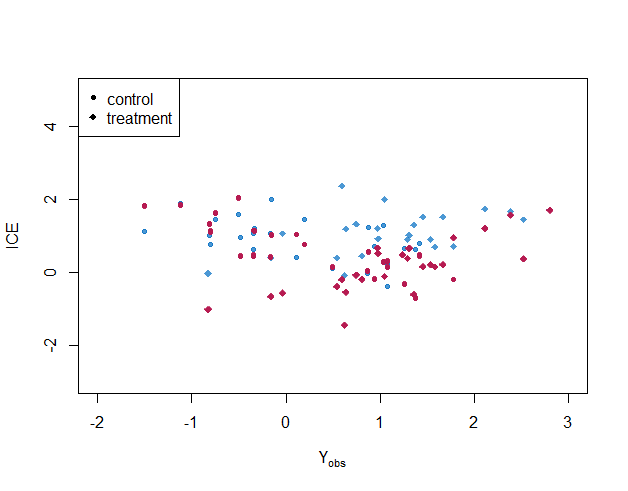
\includegraphics[scale=.5]{plots/plot4.9}
				}
			}
		\end{center}
		\caption{Stripplot of $\texttt{m} = 5$ of observed (blue) and imputed (red) data for individual treatment effects with selected cases.}
		\label{fig4_4}
	\end{figure}
	Figure \ref{fig4_4} shows posterior distributions of individual treatment effects for selected cases($\emph{i} = 100, 200, \dots, 5000$). When the partial correlation is specified correctly, the imputations look plausible: imputed ITE covers the \emph{true} ITE for almost every case, and the variance of ITE for each individual is smaller than the case under the independent conditional correlation assumption. With homogeneous treatment effect assumption, i.e., $\rho_{Y(0)Y(1)\,|\ X} = 0.99$, the imputed individual treatment effects are biased towards the average treatment effect. For targeted learning, uncertainty about the missing outcomes is not estimated. 
	
	Furthermore, we evaluate the imputations with all possible positive partial correlation (range from 0 to 1) by mean distance between the \emph{true} and the mean estimated individual treatment effects and the rate of the posterior distribution of imputed outcome cover the \emph{true} value. Fig \ref{fig4_5} shows that the violation of the homogeneous treatment effect assumption leads to extremely poor coverage. If we specified the partial correlation closed to the \emph{true} value, the imputed outcomes would be more accurate (see Fig \ref{fig4_6}). Fig \ref{fig4_6} also highlight the mean distance calculated by the targeted learning, which implies the implicit assumption of conditional independence between potential outcomes. 
	\begin{figure}[ht!]
		\centering
		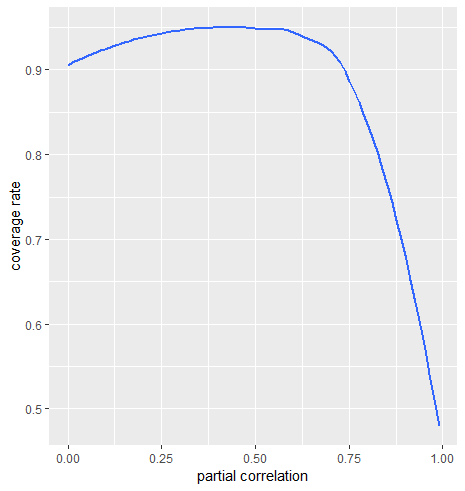
\includegraphics{plots/ICE.COVER} 
		\caption{Coverage rate of the posterior distribution of estimated individual treatment effects}
		\label{fig4_5}
	\end{figure}
	\begin{figure}[ht!]
		\centering
		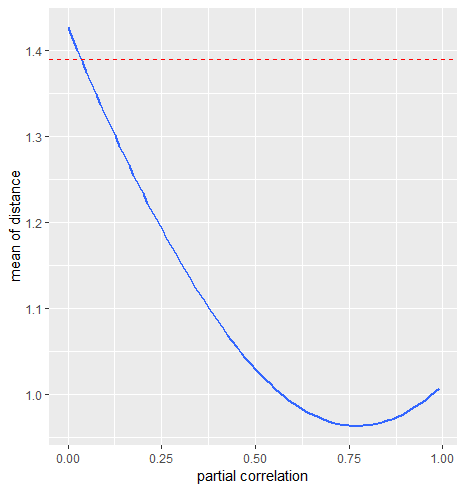
\includegraphics{plots/ICE.DIS} 
		\caption{Mean distance between the \emph{true} and the mean estimated individual treatment effects. The red dashed line represents the mean distance calculated by the targeted learning approach.}
		\label{fig4_6}
	\end{figure}
	
	The SPC approach derives the distribution of individual treatment effects, which provides more information on treatment recommendations. For instance, with a small individual treatment effect, it is possible to estimate the probability of a positive treatment effect from the distribution of individual treatment effects. 
		
	\subsubsection{Average causal inference}
	In this section, we investigate whether we could provide valid inferences for the distribution of the potential outcomes. In addition, we are interested in the biases and the coverage of nominal 95\% confidence intervals of all parameters related to the potential outcomes.  
	\begin{table}[ht!]
		\centering
		\begin{tabular}{lccc}
			Method & Truth & Est   & Cover \\
			\hline
			SPC $\rho_{partial} = 0$       &      &      &  \\\hline
			E($y_0$)       & 0.0     & 0.00     & 0.95 \\
			E($y_1$)       & 1.0     & 1.00     & 0.94 \\
			Var($y_0$)     & 1.0     & 1.00 & 0.94 \\
			Var($y_1$)     & 1.0     & 1.00 & 0.94 \\
			Cov($y_0$, $y_1$) & 0.8   & 0.25   & 0.00 \\
			Cov($y_0$, $x$)  & 0.5   & 0.50 & 0.94 \\
			Cov($y_1$, $x$)  & 0.5   & 0.50   & 0.95\\\hline
			SPC $\rho_{partial} = 0.73$       &      &      &  \\\hline
			E($y_0$)       & 0.0     & 0.00     & 0.97 \\
			E($y_1$)       & 1.0     & 1.00     & 0.95 \\
			Var($y_0$)     & 1.0     & 1.00 & 0.94 \\
			Var($y_1$)     & 1.0     & 1.00 & 0.95 \\
			Cov($y_0$, $y_1$) & 0.8   & 0.80   & 1.00 \\
			Cov($y_0$, $x$)  & 0.5   & 0.50 & 0.95 \\
			Cov($y_1$, $x$)  & 0.5   & 0.50   & 0.94\\\hline
			SPC $\rho_{partial} = 0.99$       &      &      &  \\\hline
			E($y_0$)       & 0.0     & 0.00     & 0.95 \\
			E($y_1$)       & 1.0     & 1.00     & 0.95 \\
			Var($y_0$)     & 1.0     & 1.00 & 0.95 \\
			Var($y_1$)     & 1.0     & 1.00 & 0.94 \\
			Cov($y_0$, $y_1$) & 0.8   & 0.99   & 0.00 \\
			Cov($y_0$, $x$)  & 0.5   & 0.50 & 0.95 \\
			Cov($y_1$, $x$)  & 0.5   & 0.50   & 0.95
		\end{tabular}
		\caption{Parameter estimates for SPC with different partial correlations}
		\label{tab4_2}
	\end{table} 
	Table \ref{tab4_2} shows all statistics relevant to the potential outcomes. Statistics involving only one potential outcome are unbiased and have valid coverage rates, which means that even with incorrect specified partial correlation, we could derive plausible marginal distribution of potential outcomes. Since the partial correlation is set before imputation and there is no information about the correlation between potential outcomes in the data, we get valid inference for the marginal correlation between potential outcomes only when we specified the partial correlation correctly.    
	
	\section{Application}
	\label{sec:4.6}
	We apply the SPC algorithm to evaluate the effects of two different therapies on slowing the progression of HIV disease. The data comes from a study comparing the effects of four therapies (zidovudine alone, didanosine alone, zidovudine plus didanosine and zidovudine and zalcitabine) on preventing the deterioration of disease in adults with HIV-1 infected patients \citep{hammer1996trial}. For simplicity, we name them treatment A(zidovudine alone), B(didanosine alone), C(zidovudine plus didanosine) and D(zidovudine and zalcitabine). The data named ACTG175 is accessible in package \texttt{speff2trial} in \texttt{R}. We restrict our analyses to treatments A and B and perform out-of-sample prediction of hypothetical effect of treatments A and B for the remaining patients that were allocated to treatments C and D. Hammer et al. concluded that treatment with didanosine is superior to treatment with zidovudine. However, the overall treatment effect was found to be insufficient to recommend the therapy to a patient, a situation that is common in many medical interventions. 
	
	A total of 693 HIV-1 infected adults with CD4 cell counts in the range of 200 to 500 per cubic millimetre were randomised into the control (N = 316) and treatment (N = 377) group, while 670 patients were treated as out-of-sample. Fifteen baseline covariates are included which assess gender, age, weight, Karnofsky score, risk factors, prior antiretroviral therapy, CD4 cell count, and CD8 T cell count. We are interested in the number of days until the first occurrence of: 1) a decline in CD4 cell count of at least 50 2) an event indicating progression to AIDS, or 3) death. The larger number of days yields a more beneficial treatment effect. The individual treatment effect is defined as the number of days under treatment B minus the number of days under treatment A. We select the value of partial correlation as 0 and 0.7 to perform the sensitivity analysis so that the result yields distinct differences. 
	
	\begin{figure}[ht!]
		\begin{center}
			\resizebox{\textwidth}{!}{
				\subfigure[BLI-SPC $\rho_{partial} = 0$]{
					\label{boxplot:i}
					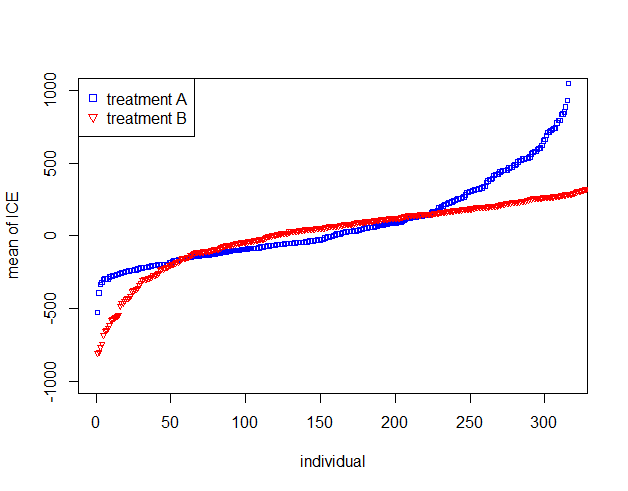
\includegraphics[scale=.5]{plots/plot4.10}
				}
				\subfigure[BLI-SPC $\rho_{partial} = 0.7$]{
					\label{boxplot:j}
					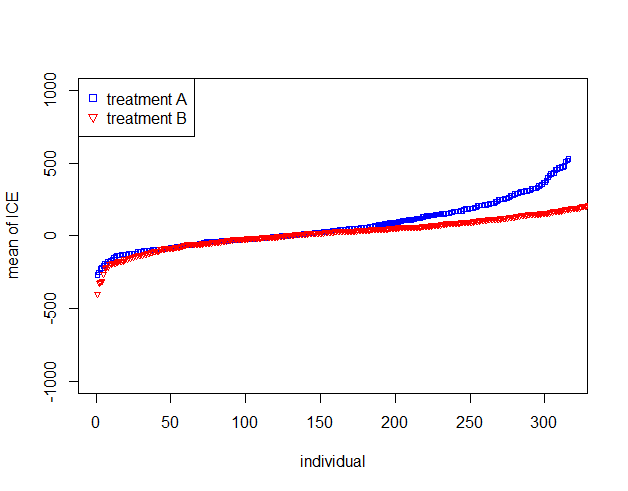
\includegraphics[scale=.5]{plots/plot4.11}
				}
			}\\
		\end{center}
		\caption{Means of individual treatment effects for patients under treatment A and treatment B, which are arranged into ascending order.}
		\label{fig4_7}
	\end{figure}
	
	\begin{figure}[ht!]
		\begin{center}
			\resizebox{\textwidth}{!}{
				\subfigure[BLI-SPC $\rho_{partial} = 0$]{
					\label{boxplot:k}
					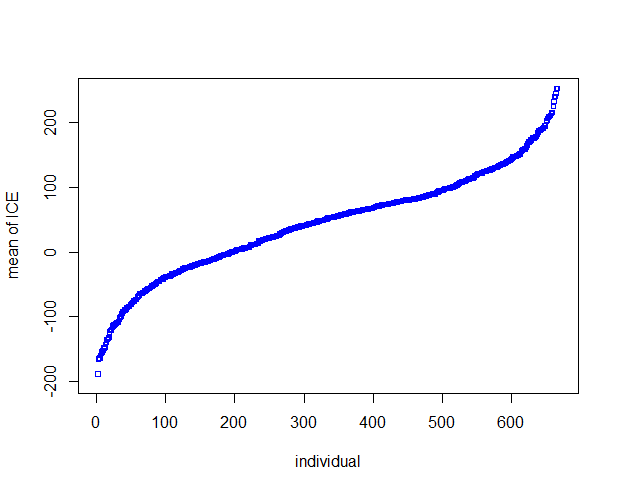
\includegraphics[scale=.5]{plots/plot4.12}
				}
				\subfigure[BLI-SPC $\rho_{partial} = 0.7$]{
					\label{boxplot:l}
					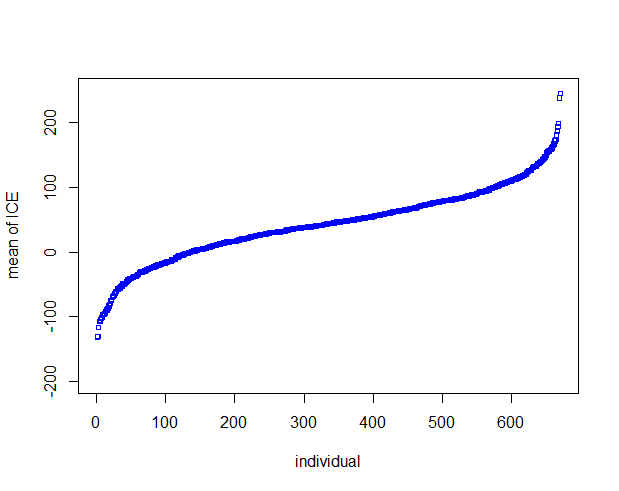
\includegraphics[scale=.5]{plots/plot4.13}
				}
			}\\
		\end{center}
		\caption{Means of individual treatment effects for out-of-sample patients under treatment C and D, which are arranged into ascending order.}
		\label{fig4_8}
	\end{figure}
	Figure \ref{fig4_7} shows the results of individual treatment effects under treatment A and treatment B group with partial correlation specification 0 and 0.7. As expected, this approach could detect the heterogeneity of treatment effects. A large proportion of patients in the sample, whose individual treatment effects are larger than 0, are recommended to receive a treatment regimen with didanosine. However, treatment with zidovudine still yields greater clinical benefit for a fraction of units, whose individual treatment effects are smaller than 0. Since all covariates are balanced under two groups, the distributions of expected individual treatment effects under two treatments (A and B) are more similar when specifying a 0.7 partial correlation. Furthermore, the range of expected value of individual treatment effects is smaller, with a partial correlation of 0.7. The larger the partial correlation we set, the more convinced that all effect modifiers are included, and effects are identical across persons. Figure \ref{4_8} shows variability in individual effects in out-of-sample patients, which implies that our method could also be applied to a prediction scenario. 
	\begin{figure}[ht!]
		\begin{center}
			\resizebox{\textwidth}{!}{
				\subfigure[]{
					\label{boxplot:m}
					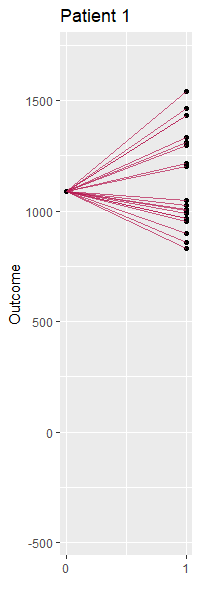
\includegraphics[scale=.5]{plots/indiv01}
				}
				\subfigure[]{
					\label{boxplot:n}
					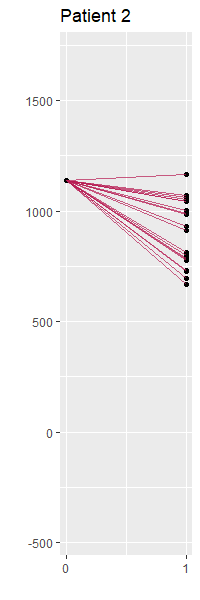
\includegraphics[scale=.5]{plots/indiv02}
				}
				\subfigure[]{
					\label{boxplot:o}
					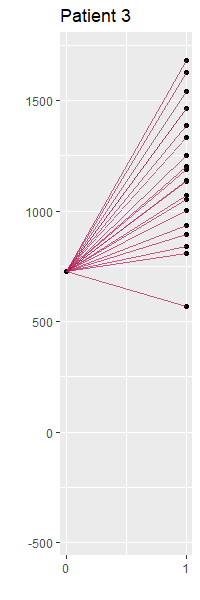
\includegraphics[scale=.5]{plots/indiv03}
				}
				\subfigure[]{
					\label{boxplot:p}
					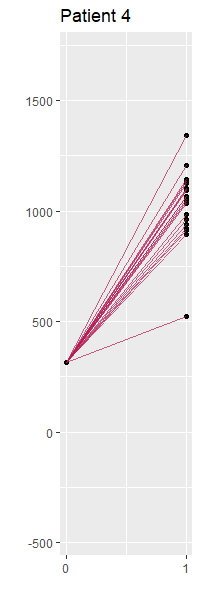
\includegraphics[scale=.5]{plots/indiv04}
				}
				\subfigure[]{
					\label{boxplot:q}
					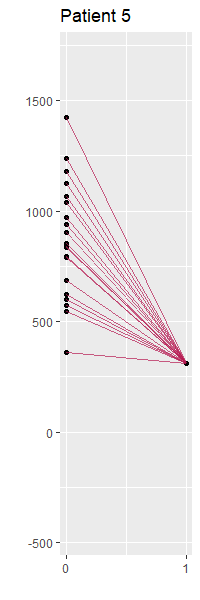
\includegraphics[scale=.5]{plots/indiv05}
				}
				\subfigure[]{
					\label{boxplot:r}
					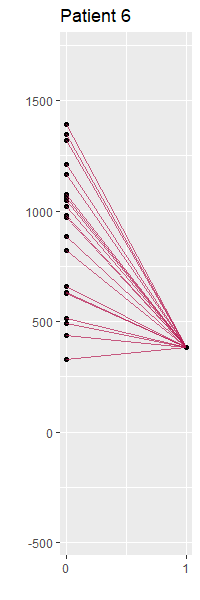
\includegraphics[scale=.5]{plots/indiv06}
				}
				\subfigure[]{
					\label{boxplot:s}
					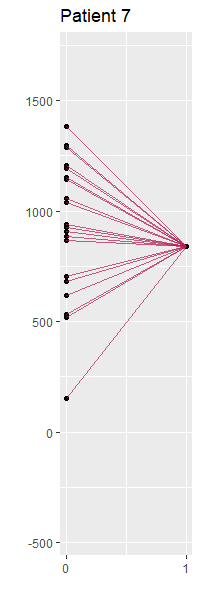
\includegraphics[scale=.5]{plots/indiv07}
				}
			}\\
		\end{center}
		\caption{Fan plot of Observed and imputed (m = 20) outcomes under treatment A (0) and B (0). The partial correlation is 0.}
		\label{fig4_9}
	\end{figure}
	
	\begin{figure}[ht!]
		\begin{center}
			\resizebox{\textwidth}{!}{
				\subfigure[]{
					\label{boxplot:t}
					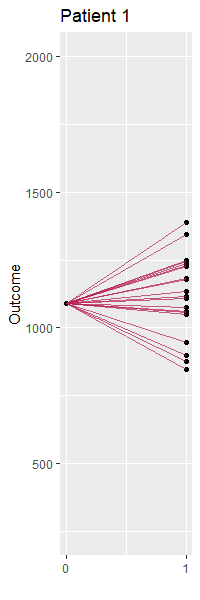
\includegraphics[scale=.5]{plots/indiv71}
				}
				\subfigure[]{
					\label{boxplot:u}
					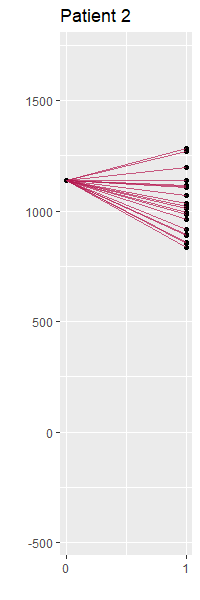
\includegraphics[scale=.5]{plots/indiv72}
				}
				\subfigure[]{
					\label{boxplot:v}
					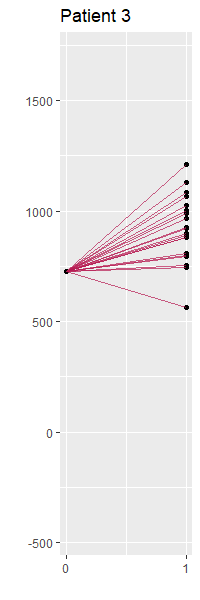
\includegraphics[scale=.5]{plots/indiv73}
				}
				\subfigure[]{
					\label{boxplot:w}
					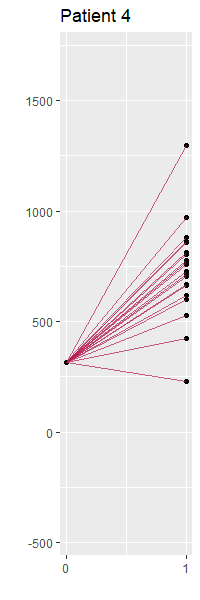
\includegraphics[scale=.5]{plots/indiv74}
				}
				\subfigure[]{
					\label{boxplot:x}
					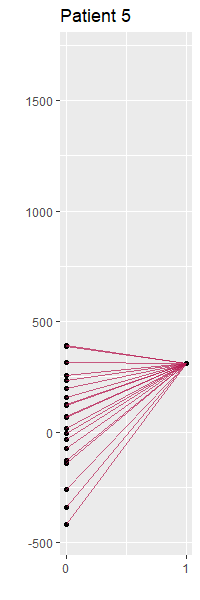
\includegraphics[scale=.5]{plots/indiv75}
				}
				\subfigure[]{
					\label{boxplot:y}
					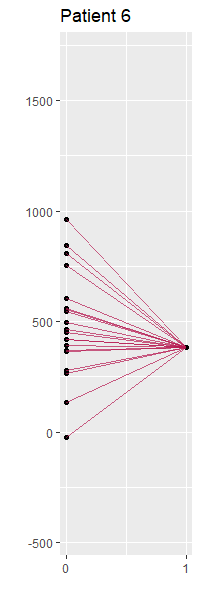
\includegraphics[scale=.5]{plots/indiv76}
				}
				\subfigure[]{
					\label{boxplot:z}
					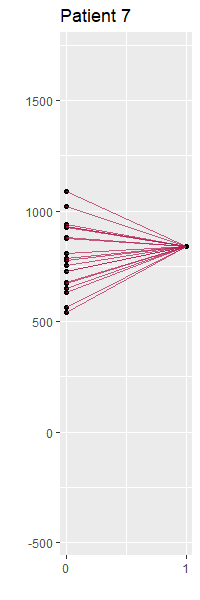
\includegraphics[scale=.5]{plots/indiv77}
				}
			}\\
		\end{center}
		\caption{Fan plot of Observed and imputed (m = 20) outcomes under treatment A (0) and B (0). The partial correlation is 0.7.}
		\label{fig4_10}
	\end{figure}
	Figure \ref{fig4_9} and \ref{fig4_10} display imputations by selected patients for two different values of partial correlation, 0 and 0.7. Each panel contains the observed outcome for the patient and $m = 20$ imputed values for the missing outcome. The imputed outcomes are sensitive to different values of partial correlation. Patient 5 benefits from treatment A when the partial correlation equals 0, while we derive the opposite conclusion when specifying the partial correlation as 0.7. The location of imputed outcomes is different under various partial correlations, and the scale shrinks when the partial correlation tends to 1.  
	
	\section{Discussion}
	\label{sec:4.7}
	We propose a multiple imputation approach to replace missing outcomes with plausible values to estimate the individual treatment effect. Treatment assignment is currently steered by the average treatment effect. This may lead to suboptimal individual treatment decisions because the treatment effects are assumed to be homogeneous. We have demonstrated that the proposed SPC algorithm allows for the imputation of heterogeneous treatment effects under a given partial correlation. 
	
	The sensitivity analysis of the partial correlation between potential outcomes in section 4.5.2 demonstrates that different values of the partial correlation yield similar results in terms of marginal distributions of potential outcomes and the average treatment effect. However, the closer the specified partial correlation is to the \emph{true} value, the less biased the estimated individual treatment effect will be. Since one cannot obtain information about the partial correlation from the observed data, the determination of the partial correlation should be set to a plausible range based on previous investigations or expert knowledge. In addition, it may be useful to perform a sensitivity analysis to see how imputed outcomes differ with different partial correlations. 
	
	An advantage of our multiple imputation approach to individual treatment effects is that it provides an estimate of the uncertainty of the imputed outcomes and hence, of the individual treatment effects. One could obtain the posterior distribution of the individual treatment effects for a unit from multiply imputed datasets, from which we can learn the probability of benefit from the treatment at the individual level. Since we incorporate the partial correlation when imputing, researchers could apply complete-data analyses to explore potential variables. This accounts for residual heterogeneity of treatment effects or additional effect modifiers. 
	
	In our illustration of the SPC algorithm, we applied Bayesian imputation under the normal linear model. It is possible to use other imputation techniques (parametric or non-parametric imputation methods). The behaviour of such methods has not yet been studied. Since SPC is a hybrid of FCS and JM, it will provide valid inferences on data that are missing at random.  Another useful property of SPC is that under the assumption of ignorable treatment assignment, researchers can skip explicit modelling of the probability of assignment. 
	
	In the application study, we focus on the comparison of treatments A and B. It is possible to generalise the multiple treatment comparison (treatment A, B, C, and D). By imputing unobserved outcomes, we could then recommend the optimal treatment to each unit among four treatments. One could benefit from our method when performing an experiment that has been investigated on a different population. Some proven effect modifiers may be difficult to collect when performing the same experiment in other regions or countries. In such a case, the inference would include the heterogeneity of treatment effects explained by the uncollected factors by specifying a reasonable partial correlation.         
	
	This is an initial study on MI to the individual treatment effect. The simulation study used a basic randomised trial with a correctly specified imputation model. Further work should be done to extend discrete and semi-continuous outcomes. Another challenge is to develop imputation techniques for studies that collect post-treatment variables. All in all, we believe that our methodology for incorporating the partial correlation represents an important advance in estimating individual treatment effects. We hope that our method may attribute to the growing body of work on personalised statistics and individual treatment effects. 

		\chapter{Joint distribution properties of Fully Conditional Specification under the normal linear model with normal inverse-gamma priors}
\chaptermark{Compatibility}
\label{chap5}
	\begin{abstract}
		Fully conditional specification (FCS) is a convenient and flexible multiple imputation approach. It specifies a sequence of simple regression models instead of a potential complex joint density for missing variables. However, FCS may not converge to a stationary distribution. Many authors have studied the convergence properties of FCS when the priors of conditional models are non-informative. We extend to the case of informative priors. This paper evaluates the convergence properties of the normal linear model with normal inverse-gamma prior. The theoretical and simulation results prove the convergence of FCS and show the equivalence of prior specification under the joint model and a set of conditional models when the analysis model is a linear regression with normal inverse-gamma priors.  
	\end{abstract}
	
	\section{Introduction}
Multiple imputation \citep{RubinD1987} is a widely applied approach for the analysis of incomplete datasets. It involves replacing each missing cell with several plausible imputed values that are drawn from the corresponding posterior predictive distributions. The most popular way to derive posterior predictive distributions' parameters is to draw randomly from the Bayesian posterior distribution of the parameters based on the observed data. In the Bayesian analysis of complete data, the researcher usually integrates their beliefs or assumptions about unknown quantities(e.g., scientific interests and parameters of the scientific models) with collected data to sharpen the conclusions. For instance, \citet{jackman2004bayesian} explained how to merge historical information with current data in an analysis of election outcomes. \citet{mccarthy2005profiting} analyzed the effect of removing spinifex on the capture rates of mulgara by incorporating results of a previous observational study. \citet{laptook2017effect} specified prior distributions on the overall treatment effects to investigate the effect of hypothermia administered between 6 and 24 hours after birth on death and disability from hypoxic-ischemic encephalopathy (HIE) because of a small sample size. However, prior information is rarely applied when drawing the parameters of the imputation model from the Bayesian posterior distribution. Non-informative priors dominate the prior specifications when conducting multiple imputation. Multiple imputation with priors beyond non-informative specification is a vast and yet unexplored field. In general, prior beliefs or assumptions to the scientific model should also be incorporated into imputation models. Potential applications could be multiple imputation of incomplete data with limited rows and multiple imputation of streaming data.  

Fully conditional specification is a popular approach to arrive at those posterior distributions under multivariate missing data. It offers a solution to this challenge by allowing a flexible specification of the imputation model for each partially observed variable. The imputation procedure then starts by imputing missing values with a random draw from the marginal distribution. Each incomplete variable is then iteratively imputed with a specified univariate imputation model. 

Although many simulation studies demonstrated that fully conditional specification yields plausible imputations in various cases, the theoretical properties of fully conditional specification are not thoroughly understood \citep{van2007multiple}. A sequence of conditional models may not imply a joint distribution to which the algorithm converges. In such a case, the imputation results may systematically differ according to different visit sequences, which is named as ``order effects" \citep{hughes2014joint}. 

Van Buuren  [2018a, Section 4.6.1] stated two cases in which FCS converges to a joint distribution. First, if all imputation models are linear with a homogenous normal distributed response, the implicit joint model would be the multivariate normal distribution. Second, if three incomplete binary variables are imputed with a two-way interaction logistic regression model, FCS would be equivalent to the joint modelling (JM) under a zero three-way interaction log-linear model. \citet{liu2014stationary} illustrated a series of sufficient conditions under which the imputation distribution for FCS converges in total variation to the posterior distribution of a joint Bayesian model when the sample size moves to infinity. Complementing the work of \citet{liu2014stationary}, \citet{hughes2014joint} pointed out that, in addition to the compatibility, a ``non-informative margins" condition is another sufficient condition for the equivalency of FCS and joint modelling for finite samples. \citet{hughes2014joint} also showed that with multivariate normal distributed data and a non-informative prior, both compatibility and the non-informative margins conditions are satisfied. In that case, fully conditional specification and joint modelling provide imputations from the same posterior distribution. \citet{zhu2015convergence} discussed conditions for convergence and assess properties of FCS. All these authors illustrated the convergence properties of FCS when the prior for conditional models is non-informative. However, the convergence property in the case of informative priors has not received much attention.       

In this paper, we focus on the question-whether the fully conditional specification (FCS) under the normal linear model with an informative inverse-gamma prior converges to a joint distribution. For the initial step to evaluate convergence properties of FCS with informative priors, it is sensible to focus on the Bayesian normal linear models and the typical informative prior: normal inverse-gamma prior. The main contributions of this paper are that we prove FCS under the normal linear model with an informative inverse-gamma prior converges to a joint distribution and provide the explicit form of the joint distribution. We hope our limited contribution could inspire others to develop more valuable research and applications about multiple imputation with informative priors. The following section will briefly overview the joint modelling, fully conditional specification, compatibility, and non-informative margins. Then, we derive a theoretical result and perform a simulation study to evaluate the non-informative margins condition. We also consider the prior for the target joint density of a sequence of normal linear models with normal inverse-gamma priors. Finally, some remarks are concluded.
	
	\section{Background}
	\subsection{Joint modelling}
	Let $Y^{obs}$ and $Y^{mis}$ denote the observed and missing data in the dataset $Y$. Joint modelling involves specifying a parametric joint model $p(Y^{obs}, Y^{mis}|\theta)$ for the complete data and an appropriate prior distribution $p(\theta)$ for the parameter $\theta$. Incomplete cases are partitioned into groups according to various missing patterns and then imputed with different submodels. Under the assumption of ignorability, the imputation model for each group is the corresponding conditional distribution derived from the assumed joint model 
	\begin{equation*}
		p(Y^{mis}|Y^{obs}) = \int_{}p(Y^{mis}| Y^{obs}, \theta)p(\theta|Y^{obs})d\theta.
	\end{equation*}
	Since the joint modelling algorithm converges to the specified multivariate distribution, once the joint imputation model is correctly specified, the results will be valid and the theoretical properties are satisfactory. 
	\subsection{Fully conditional specification}
	Fully conditional specification attempts to define the joint distribution\\$p(Y^{obs}, Y^{mis}|\theta)$ by positing a univariate imputation model for each partially observed variable. The imputation model is typically a generalized linear model selected based on the nature of the missing variable (e.g., continuous, semi-continuous, categorical, and count). Starting from some simple imputation methods, such as mean imputation or a random draw from the sampled values, FCS algorithms iteratively repeat imputations over all missing variables. Let $Y_{j}^{t} = (Y_{j}^{obs}, Y_{j}^{mis(t)})$ denote the observed and imputed values of variable $Y_{j}$ at iteration $t$ and $Y_{-j}^{t} = (Y_{1}^{t}, \dots, Y_{j-1}^{t}, Y_{j+1}^{t-1}, \dots, Y_{p}^{t-1})$. The \emph{t}th iteration for the incomplete variable \emph{$Y_{j}^{mis}$} consists of the following draws:
	\begin{align*}
		\theta_{j}^{t} \sim f(\theta_{j})f(Y_{j}^{obs}|Y_{-j}^{t}, \theta_{j})\\
		Y_{j}^{mis(t)} \sim f(Y_{j}^{mis}|Y_{-j}^{t}, \theta_{j}^{t}),
	\end{align*}
	where $f(\theta_{j})$ is generally specified with a noninformative prior. After a sufficient number of iterations, typically ranging from 5 to 10 iterations \citep{Buuren2018, oberman2020missing}, the stationary distribution is achieved. The final iteration generates a single imputed dataset and multiple imputations are created by applying FCS in parallel \emph{m} times with different seeds. If the underlying joint distribution defined by separate conditional models exists, the algorithm is equivalent to a Gibbs sampler. 
	
	The attractive feature of fully conditional specification is the flexibility of model specification, which allows models to preserve features in the data, such as skip patterns, incorporating constraints, logistical and consistency bounds \citep{van2007multiple}. Such restrictions would be difficult to formulate when applying joint modelling. One could conveniently construct a sequence of conditional models and avoid the specification of a parametric multivariate distribution, which may not be appropriate for the data in practice.
	
	Fully conditional specification has been proposed under a variety of names: chained equations stochastic relaxation, variable-by-variable imputation, switching regression, sequential regressions, ordered pseudo-Gibbs sampler, partially incompatible MCMC and iterated univariate imputation \citep[Section 4.5.1]{Buuren2018}. Fully conditional specification can be of great value in practice because of its flexibility in model specification. FCS has become a standard in practice and has been widely implemented in software (e.g. \texttt{mice} and \texttt{mi} in \texttt{R}, \texttt{IVEWARE} in \texttt{SAS}, \texttt{ice} in \texttt{STATA} and module \texttt{MVA} in \texttt{SPSS}) \citep{Buuren2011}.
	
	\subsection{Compatibility} 
	The definition of compatibility is given by \citet{liu2014stationary}: let $Y = (Y_1, Y_2, \dots, Y_p)$ be a vector of random variables and $Y_{-j} = (Y_1, Y_2, \dots, Y_{j-1}, Y_{j+1}, \dots, Y_{p})$. A set of conditional models $\{f_{j}(Y_j|Y_{-j}, \theta_{j}) : \theta_{j} \in \Theta_{j}, j = 1, 2, \dots, p\}$ is said to be compatible if there exists a joint model $\{\emph{f}(Y|\theta) : \theta \in \Theta\}$ and a collection of surjective maps $\{t_{j} : \Theta \to \Theta_{j}\}$ such that for each $j$, $\theta_{j} \in \Theta_{j}$ and $\theta \in t_{j}^{-1}(\theta_{j}) = \{\theta : t_{j}(\theta) = \theta_{j}\}$. In that case 
	\begin{gather*}
		f_{j}(Y_j|Y_{-j}, \theta_{j}) = \emph{f}(Y_j|Y_{-j}, \theta).
	\end{gather*}
	Otherwise, $\{f_{j}, j = 1, 2, \dots, p\}$ is said to be incompatible.
	A simple example of compatible models is a set of normal linear models for a vector of continuous data: 
	\begin{gather*}
		Y_j = N((\textbf1, Y_{-j})\beta_{j}, \sigma_{j}^2), 
	\end{gather*}
	where $\beta_{j}$ is the vector of coefficients and $\textbf1$ is a vector of ones. In such a case, the joint model of $(Y_1, Y_2, \dots, Y_p)$ would be a multivariate normal distribution and the map $t_j$ is derived by conditional multivariate normal formula. On the other hand, the classical example for an incompatible model would be the linear model with squared terms \citep{liu2014stationary, bartlett2015multiple}.
	
	Incompatibility is a theoretical weakness of fully conditional specification since, in some cases, it is unclear whether the algorithm indeed converges to the desired multivariate distribution \citep{arnold1989compatible, arnold2004compatibility, heckerman2000dependency, van2006fully}. Consideration of compatibility is significant when the multivariate density is of scientific interest. Both \citet{hughes2014joint} and \citet{liu2014stationary} stated the necessity of model compatibility for the algorithm to converge to a joint distribution. Several papers introduced some cases in which FCS models are compatible with joint distributions \citep{Buuren2018, raghunathan2001multivariate}. \citet{van2006fully} also performed some simulation studies of fully conditional specification with strongly incompatible models and concluded the effects of incompatibility are negligible. However, further work is necessary to investigate the adverse effects of incompatibility in more general scenarios. 
	
	\subsection{Non-informative margins}
	\citet{hughes2014joint} showed that the non-informative margins condition is sufficient for fully conditional specification to converge to a multivariate distribution. Suppose $\pi(\theta_{j})$ is the prior distribution of the conditional model $p(Y_j|Y_{-j}, \theta_{j})$ and $\pi(\theta_{-j})$ is the prior distribution of the marginal model $p(Y_{-j}|\theta_{-j})$, then the non-informative margins condition is satisfied if the joint prior could be factorized into independent priors $\pi(\theta_{j}, \theta_{-j}) = \pi(\theta_{j})\pi(\theta_{-j})$. It is worthwhile to note that the non-informative margin condition does not hold if $p(Y_j|Y_{-j}, \theta_{j})$ and $p(Y_{-j}|\theta_{-j})$ have the same parameter space. When the non-informative margins condition is violated, an order effect appears. In such a case, the inference of parameters would have systematic differences depending on the sequence of the variables in FCS algorithm. Simulations performed by \citet{hughes2014joint} demonstrated that such an order effect is subtle. However, more research is needed to verify such claims, and it is necessary to be aware of the existence of the order effect. 
	
	\section{Theoretical results}
	Under weak regularity conditions, FCS under the normal linear model with an informative inverse-gamma prior converges to a joint distribution. This section provides the proof of that claim. Since the compatibility of the normal linear model is well understood,  we will check the satisfaction of the non-informative margins condition. 
	
	Starting with the problem of Bayesian inference for $\theta = (\mu, \Sigma)$ under a multivariate normal model, let us apply the following prior distribution. Suppose that, given $\Sigma$, the prior distribution of $\mu$ is assumed to be the conditionally multivariate normal,
	\begin{equation}
		\mu | \Sigma \sim N(\mu_{0}, \tau^{-1}\Sigma),
	\end{equation}
	where the hyperparameters $\mu_{0} \in \mathcal{R}^{p}$ and $\tau > 0$ are fixed and known and where $p$ denotes the number of variables. Moreover, suppose that the prior distribution of $\Sigma$ is an inverse-Wishart,
	\begin{equation}
		\Sigma \sim W^{-1}(m, \Lambda),
	\end{equation}
	for fixed hyperparameters $m \ge p$ and $\Lambda$. The prior density for $\theta$ can then be written as
	\begin{equation}
		\begin{array}{ll}
			\pi(\theta) \propto &|\Sigma|^{-(\frac{m+p+2}{2})}\;\exp\;\{-\frac{1}{2}tr(\Lambda^{-1}\Sigma^{-1})\}\\
			& \times\;\exp\;\{-\frac{\tau}{2}(\mu-\mu_{0})^{T}\Sigma^{-1}(\mu-\mu_{0})\}.
		\end{array}	
	\end{equation}
	For each variable $Y_{j}$, we partition the mean vector $\mu$ as $(\mu_j, \mu_{-j})^T$ and the covariance matrix $\Sigma$ as 
	\begin{eqnarray*}
		\left(\begin{array}{cc}
			\omega_{j} & \xi_{j}^T\\
			\xi_{j} & \Sigma_{-j} 
		\end{array}\right),
	\end{eqnarray*}
	such that $Y_j \sim \mathcal{N}(\mu_j, \omega_{j})$ and $Y_{-j} \sim \mathcal{N}(\mu_{-j}, \Sigma_{-j})$. Similarly, we partition the scale parameter $\mu_{0}$ as $(\mu_{0j}, \mu_{0-j})^T$ and $\Lambda$ as
	\begin{eqnarray*}
		\left(\begin{array}{cc}
			\Lambda_{j} & \psi_{j}^T\\
			\psi_{j} & \Lambda_{-j} 
		\end{array}\right).
	\end{eqnarray*}
	The conditional model of $Y_j$ given $Y_{-j}$ is the normal linear regression $Y_{j} = \alpha_j + \beta_{j}^TY_{-j} + \sigma_{j}$, where $\beta_{j}^T = \xi_{j}^T\Sigma_{-j}^{-1}$, $\alpha_j = \mu_j - \xi_{j}^T\Sigma_{-j}^{-1}\mu_{-j}$ and $\sigma_{j} = \omega_{j} - \xi_{j}^T\Sigma_{-j}^{-1}\xi_{j}$. The corresponding vectors of parameters $\theta_{j}$ and $\theta_{-j}$ would be 
	\begin{equation}
		\begin{array}{cc}
			\theta_{j}  &= (\alpha_j, \beta_{j}, \sigma_{j})\\
			\theta_{-j} &= (\mu_{-j}, \Sigma_{-j}).
		\end{array}
	\end{equation}
	By applying the partition function illustrated by \citet[p. 165]{Eation2007} and by block diagonalization of a partitioned matrix, the joint prior for $\theta_{j}$ and $\theta_{-j}$ can be derived from $\pi(\theta)$ as :
	\begin{equation}
		\begin{array}{l}
			\pi(\theta_{j}, \theta_{-j}) = p(\sigma_{j})p(\beta_{j}|\sigma_{j})p(\Sigma_{-j})\\
			\times \exp\;\{-\frac{\tau}{2}(\alpha_{j} + \beta_{j}\mu_{0-j}\ - \mu_{0j})^{T}(\sigma_{j})^{-1}(\alpha_{j} + \beta_{j}\mu_{0-j}\ - \mu_{0j})\}\\
			\times \exp\{-\frac{\tau}{2}(\mu_{-j}-\mu_{0-j})^{T}\Sigma_{-j}^{-1}(\mu_{-j}-\mu_{0-j})\} \times |\Sigma_{-j}|\\
			=\pi(\theta_{j})\pi(\theta_{-j}),
		\end{array}
	\end{equation}
	where
	\begin{align}
		&\pi(\theta_{j}) = p(\sigma_{j})p(\beta_{j}|\sigma_{j}) \nonumber\\
		&\times \exp\;\{-\frac{\tau}{2}(\alpha_{j} + \beta_{j}\mu_{0-j}\ - \mu_{0j})^{T}(\sigma_{j})^{-1}(\alpha_{j} + \beta_{j}\mu_{0-j}\ - \mu_{0j})\},\\
		&\pi(\theta_{-j}) = p(\Sigma_{-j})\times \exp\{-\frac{\tau}{2}(\mu_{-j}-\mu_{0-j})^{T}\Sigma_{-j}^{-1}(\mu_{-j}-\mu_{0-j})\} \times |\Sigma_{-j}|,
	\end{align}
	and 
	
	$p(\sigma_{j}) \sim W^{-1}(m, \lambda_j)$, $p(\beta_{j}|\sigma_{j}) \sim \mathcal{N}(\psi_{j}^T\Lambda_{-j}^{-1}, \lambda_j\Lambda_{-j}^{-1})$, $p(\Sigma_{-j}) \sim W^{-1}(m-1, \Lambda_{-j})$, $\lambda_j = \Lambda_{j} - \psi_{j}^T\Lambda_{-j}^{-1}\psi_{j}$ (Eaton, 2007, Section 8.2). Since the joint prior distribution factorizes into independent priors, the ``non-informative" margins condition is satisfied and the validity of our claim that FCS under the normal linear model with an informative inverse-gamma prior converges to a joint distribution is demonstrated. 
	
	Based on equations (6) and (7), we could also derive the connection between the prior for the conditional linear model and the prior for the corresponding joint distribution:
	\begin{equation}
		\begin{array}{l}
			p(\sigma_{j}) \sim W^{-1}(m, \lambda_j)\\
			p(\beta_{j}|\sigma_{j}) \sim \mathcal{N}(\psi_{j}^T\Lambda_{-j}, \lambda_j\Lambda_{-j})\\
			p(\alpha_{j}|\sigma_{j}) \sim \mathcal{N}(\mu_{0j} - \psi_{j}^T\Lambda_{-j}\mu_{02}, \tau^{-1}\sigma_{j} - (\mu_{-0j})^{2}\lambda_j\Lambda_{-j}^{-1}).
		\end{array}
	\end{equation} 
	Since the conditional $\beta_{j} | \sigma_{j}$ follows a normal distribution, the marginal distribution $\beta_{j}$ would be a student's t-distribution $\beta_{j} \sim t(\psi_{j}^T\Lambda_{-j}^{-1}, \\m\Lambda_{-j}^{-1}\lambda_{j}^{-1}, 2m-p+1)$. When the sample size increases, $\beta_{j}$ tends to the normal distribution $N(\psi_{j}^T\Lambda_{-j}^{-1}, \frac{\lambda_{j}\Lambda_{-j}}{m-1})$. Similarly, the marginal distribution $\alpha_{j}$ would be $t(\mu_{0j} - \psi_{j}^T\Lambda_{-j}\mu_{02}, m(\tau^{-1} - (\mu_{0-j})^{2}\Lambda_{-j}^{-1})\Lambda_{j}^{-1}, 2m-p+1)$. When the sample size increases, $\alpha_{j}$ tends to the normal distribution $N(\mu_{0j} - \psi_{j}^T\Lambda_{-j}\mu_{02},\\
	\frac{1}{(\tau^{-1} - (\mu_{-0j})^{2}\Lambda_{-j}^{-1})(m-1)}\Lambda_{j})$. Usually, when the sample size is over 30, the difference between student's t-distribution and the corresponding normally distributed approximation is negligible. With the prior transformation formula, one could apply Bayesian imputation under the normal linear model even with prior information of the mean vector and the covariance matrix of the incomplete data.   
	
	\section{Simulation}
	We perform a simulation study to demonstrate the validity and convergence of fully conditional specification when the conditional models are simple linear regressions with an inverse-gamma prior for the error term and a multivariate normal prior for regression weights. In addition, we look for the disappearance of order effects, which is evident in the convergence of fully conditional specification to a multivariate distribution. 
	
	We repeat the simulation 500 times and generate a dataset with 200 cases for every simulation according to the following multivariate distribution :
	\begin{eqnarray*}
		\begin{pmatrix}x\\
			y\\
			z
		\end{pmatrix} & \sim & \mathcal{N}\left[\left(\begin{array}{c}
			1\\
			4\\
			9
		\end{array}\right),\left(\begin{array}{ccc}
			4 & 2 & 2\\
			2 & 4 & 2\\
			2 & 2 & 9 
		\end{array}\right)\right].\\
	\end{eqnarray*}
	Fifty percent missingness is induced on either variable $x$, $y$ or $z$. The proportion of the three missing patterns is equal. When evaluating whether it is appropriate to specify a normal inverse-gamma prior, we consider both missing completely at random (MCAR) mechanisms and right-tailed missing at random (MARr) mechanisms where higher values have a larger probability to be unobserved. When investigating the existence of order effects, we only conduct the simulation under MCAR missingness mechanism to ensure that the missingness does not attribute to any order effects. We specify a weak informative prior for two reasons. First, with a weak informative prior, the frequentist inference is still plausible by applying Rubin's rules \citep[p. 76]{RubinD1987}. Second, \citet{Goodrich2019} suggested that compared with flat non-informative priors, weak informative priors place warranted weight to extreme parameter values. In such a case, the prior under the joint model is specified as: $\mu_{0} = (0, 0, 0)^T$, $\tau = 1$, $m = 3$ and 
	\begin{eqnarray*}
		\Lambda = \left(\begin{array}{ccc}
			60 & 0 & 0\\
			0 & 60 & 0\\
			0 & 0 & 60 
		\end{array}\right),
	\end{eqnarray*}
	and the corresponding prior for separated linear regression model would be the same, with $\pi(\sigma) \sim W^{-1}(3, 60)$ and 
	\begin{eqnarray*}
		(\alpha, \beta)^T
		& \sim & \mathcal{N}\left[\left(\begin{array}{c}
			0\\
			0\\
			0
		\end{array}\right),\left(\begin{array}{ccc}
			60 & 0 & 0\\
			0 & 3600 & 0\\
			0 & 0 & 3600 
		\end{array}\right)\right].\\
	\end{eqnarray*}
	\subsection{Scalar inference for the mean of variable Y}
	The aim is to assess whether Bayesian imputation under a normal linear model with normal inverse-gamma priors would yield unbiased estimates and exact coverage of the nominal 95\% confidence intervals. Table \ref{tab5_1} shows that with weak informative prior, fully conditional specification also provides valid imputations. The estimates are unbiased, and the coverage of the nominal 95\% confidence intervals is correct under both MCAR and MARr. Without the validity of a normal inverse-gamma prior specification, further investigations into the convergence would be redundant. 
	\begin{table}[h]
		\centering
		\vspace{0.5cm}
		\begin{tabular}{ccccc}
			& Bias  & Cov  & Ciw &  \\
			MCAR & 0     & 0.95 & 0.74 &  \\
			MARr & -0.01 & 0.97 & 0.73 &  \\
			&       &      &  & 
		\end{tabular}
		\caption{Bias of the estimates ($E(Y)$) and coverage of nominal 95\% confidence intervals under MCAR and MARr}
		\label{tab5_1}
	\end{table}
	
	\subsection{Order effect evaluation}
	The visit sequence laid upon the simulation is $z$, $x$ and $y$. To identify the presence of any systematic order effect, we estimate the regression coefficient directly after updating variable $z$ and after updating variable $x$. Specifically, the \emph{i}th iteration of fully conditional specification would be augmented as:
	\begin{enumerate}
		\item impute $z$ given $x^{i-1}$ and $y^{i-1}$.
		\item build the linear regression $y = \alpha + \beta_{1}x + \beta_{2}z + \epsilon$ and collect the coefficient $\beta_{1}$, denoted as $\hat{\beta}^z_{1}$.
		\item impute $x$ given $z^{i}$ and $y^{i-1}$.
		\item build the linear regression $y = \alpha + \beta_{1}x + \beta_{2}z + \epsilon$ and collect the coefficient $\beta_{1}$, denoted as $\hat{\beta}^x_{1}$.
		\item impute $y$ given $z^{i}$ and $x^{i}$.	 
	\end{enumerate}
	After a burn-in period with 10 iterations, the fully conditional specification algorithm was performed with an additional 1000 iterations, in which differences between the estimates $\hat{\beta}^z_{1} - \hat{\beta}^x_{1}$ are recorded. The estimates from the first 10 iterations are omitted since the FCS algorithms commonly reach convergence around 5 to 10 iterations. Estimates from the additional 1000 iterations would be partitioned into subsequences with equal size, which are used for variance calculation. We calculate the nominal 95\% confidence interval of the difference. The standard error of the difference is estimated with batch-means methods \citep[p. 124]{albert2009bayesian}. The mean of $\hat{\beta}^z_{1} - \hat{\beta}^x_{1}$ is set to zero. Since only three 95\% confidence intervals derived from 500 repetitions do not include the zero, there is no indication of any order effects. We also monitor the posterior distribution of the coefficient under both joint modelling and fully conditional specification. Figure \ref{fig5_1} shows a quantile-quantile plot demonstration the closeness of the posterior distribution for $\beta_{1}$ derived from both joint modelling and fully conditional specification. Since the posterior distributions for $\beta_{1}$ under joint modelling and FCS are very similar, any differences may be considered negligible in practice.  
	\begin{figure}[h]
		\centering
		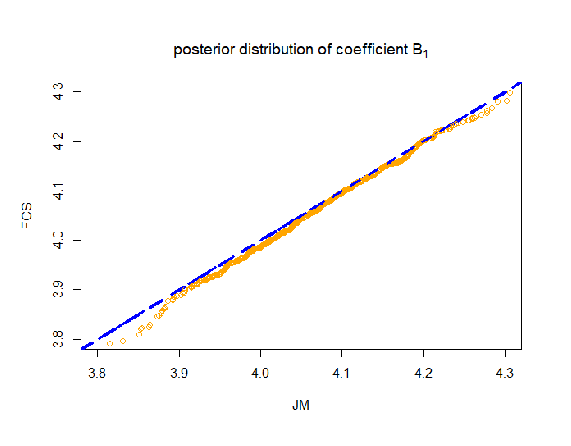
\includegraphics[scale=0.7]{plots/plot5.1.eps}
		\caption{qqplot demonstrating the closeness of the posterior distribution of JM and FCS for $\beta_{1}$}
		\label{fig5_1}
	\end{figure} 
	
	All these results confirm that under the normal inverse-gamma prior, Bayesian imputation under normal linear model converges to the corresponding multivariate normal distribution. 
	
	\section{Conclusion}
	In this paper, we study the problem of whether fully conditional specification under the normal linear model with normal inverse-gamma prior converges to a joint distribution. Based on the theory of the non-informative margins condition proposed by \citet{hughes2014joint}, we demonstrate the validity of the convergence. We also provide the equivalence relation between a sequence of normal inverse-gamma priors for fully conditional specification and a normal inverse-Wishart for joint modelling. It allows the imputer to merge prior beliefs about the mean vector and the covariance matrix of the incomplete data when applying FCS to impute. 
	
	Fully conditional specification is an appealing imputation method because it allows one to specify a sequence of flexible and simple conditional models and bypass the difficulty of multivariate modelling in practice. The default prior for normal linear regression is Jeffreys prior, which satisfies the non-informative margin condition. However, it is worth developing other types of priors for fully conditional specification such that one could select the prior, which suits the description of prior knowledge best. Many researchers have discussed the convergence condition of FCS. However, there is no conclusion for the family of posterior distributions that satisfies the condition of convergence. In such a case, when including new kinds of priors in fully conditional specification algorithms, it is necessary to investigate the convergence of the algorithm with new posterior distributions. Specifically, one should study the non-informative margin conditions for new priors. Compatibility should also be considered if the imputation model is novel. Our work takes steps in this direction. 
	
	Although a series of investigations have shown that the adverse effects of violating compatibility and non-informative margin conditions may be small, all of these investigations rely on predefined simulation settings. More research is needed to verify the conditions under which the fully conditional specification algorithm converges to a multivariate distribution and cases in which the violation of compatibility and non-informative margin has negligible adverse impacts on the result.
	
	
	There are several directions for future research. From one direction, it is possible to develop a prior setting to eliminate the order effects of the fully conditional specification algorithm under the general location model since the compatibility and non-informative margins conditions are satisfied under the saturated multinomial distribution. Moreover, various types of priors of the generalized linear model for the fully conditional specification and corresponding joint modelling rationales could be developed. Another open problem is the convergence condition and properties of block imputation, which partitions missing variables into several blocks and iteratively imputes blocks \citep[Section 4.7.2]{Buuren2018}. Block imputation is a more flexible and user-friendly method. However, its properties have yet to be studied. Finally, it is necessary to investigate the implementation of prior specifications in software.         
	
	

		\include{parts/part3}
		\chapter{Graphical and numerical diagnostic tools to assess multiple imputation models by posterior predictive checking}
\chaptermark{Diagnostics for imputation models}
\label{chap6}
	\begin{abstract}
		We propose a method to diagnose imputation models based on posterior predictive checking. To assess the congeniality of imputation models, we compare the observed data with their replicates generated under corresponding posterior predictive distributions. The idea is that if the imputation model is congenial with the substantive model, the observed data is expected to locate in the centre of corresponding predictive posterior distributions. We investigate the proposed diagnostic method for parametric and non-parametric imputation approaches, continuous and discrete incomplete variables, univariate and multivariate missingness patterns. The results show the validity of the proposed diagnostic method.  	
	\end{abstract}
	
	\section{Introduction}
	\label{sec:6.1}
	Multiple imputation (MI) is a popular approach for the analysis of incomplete datasets. It involves generating several plausible imputed datasets and aggregating different results into a single inference. Missing cells are filled with synthetic data drawn from corresponding posterior predictive distributions. This procedure is repeated multiple times, resulting in several imputed datasets. The parameters of scientific interest are then estimated for each imputed dataset by complete-data analyses. Finally, different estimates are pooled into one inference using Rubin's rule, which accounts for within and across imputation uncertainty \citep{RubinD1987}. 
	
	A crucial part of the multiple imputation process is selecting sensible models to generate plausible values for the missing data. The validity of post-imputation analyses relies on the congeniality of the imputation model and the substantive model of interest \citep{meng1994multiple}. However, model selection is not a trivial process in practice since there can be a wide array of candidate models to check. Therefore, researchers should consider which variables, interaction terms, and nonlinear terms are included based on the scientific interest and data features.  
	
	Despite the popularity of multiple imputation, there are only a few imputation model diagnostic methodologies. One standard diagnostic method is to compare distributions of the observed with imputed data \citep{Buuren2018, abayomi2008diagnostics}. Plausible imputation models would generate imputed values that have a similar distribution to the observed data. Although missing at random (MAR) mechanisms would also induce the discrepancies between the observed and imputed data, any dramatic departures that the observed data features cannot explain are evidence of potential imputation model misspecification. Reliable interpretation of the observed and imputed data's discrepancies could be derived from external knowledge about the incomplete variables and the missingness mechanisms \citep{abayomi2008diagnostics}. 
	
	The idea to evaluate the validity of scientific models with multiply imputed data is not new. \citet{bondarenko2016graphical} proposed an advanced diagnostic method to compare the distributions of the observed with imputed data conditional on the probability of missingness. \citet{gelman1998not} applied cross-validation to check the fit of a hierarchical Bayesian model in the study of 51 public opinion polls preceding the 1988 U.S. Presidential election. \citet{gelman2005multiple} also proposed to apply graphical posterior predictive inference on the test statistics for model checking with missing and latent data. If regression-based imputation approaches are involved, the conventional regression diagnostics, such as plots of residuals and outliers, are helpful \citep{white2011multiple}. A comprehensive overview of model diagnostic in multiple imputation is available in \citet{nguyen2017model}.
	
	Posterior predictive checking (PPC) has been proposed as an alternative method for the imputation model diagnostic \citep{gelman2005multiple, he2012diagnosing, nguyen2015posterior}. PPC is a Bayesian model checking approach that compares the replicated data drawn from the corresponding posterior predictive distribution to the observed data. If the model lacks fit, there could be a discrepancy between the replicated and observed data. 
	
	\citet{he2012diagnosing} and \citet{nguyen2015posterior} applied posterior predictive checking to assess the inadequacies of the joint imputation model with one or more test quantities relative to the scientific interest. To evaluate the `usability' of imputation models with respect to the test statistics, analysts compare the estimates for the complete data to their replicates. Comparisons of the complete data and its replicates ensure the calculation of test quantities with general missingness patterns. However, it also results in sensitivity to the amount of missingness.    
	
	This manuscript proposes and evaluates the implementation of posterior predictive checking for imputation techniques. The general idea is that if the imputation model is congenial to the substantive model, the expected value of the data (whether observed or missing) is in the centre of corresponding predictive posterior distributions. We compare the observed data to their posterior replicates generated under the imputation model and evaluate the posterior distributions of all observed data points. This distinguishes our approach from the posterior predictive checking of imputation models by applying target analyses. We demonstrate:
	\begin{enumerate}
		\item that PPC can be generalised to variable-by-variable imputation techniques; 
		\item that PPC can be used to identify the imputation model that conforms most to the true data generating model;
		\item that PPC can be used as a model evaluation technique to identify the better substantive analysis model;
		\item how to perform PPC with \texttt{MICE} in \texttt{R} on a real-life data set \citep{Buuren2011};
		\item that this PPC approach is not sensitive to the amount of missing data.
	\end{enumerate}
	The remainder of this manuscript is organised as follows. In section \ref{sec:6.2}, we review the posterior predictive checking of the imputation model by applying the target analysis proposed by \citet{he2012diagnosing}. In section \ref{sec:6.3}, we provide an overview of the \texttt{MICE} package and the underlying imputation algorithm: fully conditional specification (FCS). We also further point out the necessity of extending the posterior predictive checking of the imputation model so that the diagnostics would apply to the \texttt{MICE} algorithm. In section \ref{sec:6.4}, we evaluate the performance of the proposed diagnostic approach with simulation studies. In section \ref{sec:6.5}, we show the results of simulation studies. In section \ref{sec:6.6}, we apply the proposed diagnostic approach to the body mass index (BMI) data in Dutch. In section \ref{sec:6.7}, we conclude with a discussion of our findings.  
	
	\section{Posterior predictive checking (PPC)}
	\label{sec:6.2}
	\subsection{Posterior predictive checking}
	Without incomplete variables, PPC compares the observed data $y$ with the replicated data $y^{rep}$ which are simulated from the posterior predictive distribution, with parameter $\theta$:
	\begin{equation}
		\begin{array}{ll}
			p(y^{rep}|y) = \int p(y^{rep}|\theta)p(\theta|y)d\theta
		\end{array} 
	\end{equation}
	To detect the discrepancy between the model and the data, we define test quantities that reflect the scientific interest and estimate them for both observed and replicated data. Misfits of the model with respect to the data could be summarised by the posterior predictive p-value, which is the probability that the replicated data are more extreme than the observed data, with respect to the selected test quantities \citep{gelman2013bayesian}:
	\begin{equation}
		\begin{array}{ll}
			p_{B} &= Pr(T(y^{rep}, \theta) \ge T(y, \theta)|y)\\
			&= \int\int I_{T(y^{rep}, \theta) \ge T(y, \theta)}p(y^{rep}|\theta)p(\theta|y)dy^{rep}d\theta,
		\end{array} 
	\end{equation}
	where $I$ is the indicator function. An extreme p-value (close to 0 or 1) implies the suspicion on the fit of the model since a consistent discrepancy between test quantities $T(y^{rep}, \theta)$ and $T(y, \theta)$ cannot be explained by the simulation variance. 
	
	Posterior predictive checking has been widely used for model diagnostic in applied Bayesian analysis \citep[chapter 6]{gelman2013bayesian}, and the posterior predictive distribution is usually calculated by simulation. Suppose we have $N$ draws of model parameters from its posterior distribution $\theta_j, j=1,\dots,N$, we then generate a replicated data for every theta $\theta_j$. The PPC compares test quantities based on observed data with the empirical predictive distribution of test quantities. The estimated posterior predictive p-value is the proportion of these \texttt{N} simulations for which $T_{j}(y^{rep}, \theta) > T_{j}(y, \theta)$. It is noticeable that PPC's application for the imputation model diagnostic is not based on the hypothesis test perspective. Hence, there is no underlying assumed distribution for the posterior predictive p-value in this case. The posterior predictive p-value indicates whether the model would provide plausible inference based on the data with respect to the selected test quantities. 
	
	To perform multiple imputation model checking with PPC, we compare the completed data, the combination of the observed and imputed data, with its replications. \citet{gelman2005multiple} applied graphical PPC to visualise test quantities comparisons based on completed and replicated data. \citet{he2012diagnosing} and \citet{nguyen2015posterior} developed numerical posterior predictive checks as target analyses to the joint imputation model. \citet{he2012diagnosing} proposed two kinds of discrepancies, completed data discrepancy and expected completed-data discrepancy, and the approaches to calculate corresponding posterior predictive p-values. We briefly introduce these discrepancies and p-values for the completeness of PPC for MI models.
	
	\subsection{Completed-data discrepancy}
	To assess the completed-data discrepancy $T(y_{com}^{rep}, \theta) - T(y_{com}, \theta)$, we draw imputed values for incomplete variables $y_{mis}$ and the replication of the complete data $y_{com}^{rep}$ from their posterior predictive distribution:
	\begin{equation}
		\begin{array}{ll}
			p(y_{com}^{rep}, y_{mis}|y_{obs}) = \int p(y_{com}^{rep}|\theta)p(y_{mis}|y_{obs}, \theta)p(\theta|y_{obs})d\theta,
		\end{array} 
	\end{equation}
	where $y_{obs}$ is the observed data and $y_{com} = (y_{obs}, y_{mis})$. To assess the model fit, we calculate the posterior predictive p-value as :
	\begin{equation}
		\begin{array}{ll}
			p_{B, com} &= Pr(T(y_{com}^{rep}) \ge T(y_{com})|y_{obs})\\
			&= \int\int I_{T(y_{com}^{rep}) \ge T(y_{com})}p(y_{com}^{rep}, y_{mis}|y_{obs})dy_{com}^{rep}dy_{mis}
		\end{array} 
	\end{equation}
	The simulation process to estimate p-value proposed by \citet{he2012diagnosing} is:
	\begin{enumerate}
		\item Simulate $N$ draws of $\theta$ from the corresponding posterior distribution $p(\theta|y_{obs})$
		\item For each $\theta_{j}, j=1, \dots, N$, impute $y_{mis}^j$ from $p(y_{mis}|y_{obs}, \theta_{j})$ and simulate the replicated data $y_{com}^{rep, j}$ from $p(y_{com}^{rep}|\theta_{j})$
	\end{enumerate}
	A $p_{B, com}$, which is close to 0 or 1, implies the discrepancy between the model and the data with respect to the selected test quantities.  
	\subsection{Expected completed-data discrepancy}
	\citet{he2012diagnosing} noticed that the power of completed-data discrepancy is weakened because the variance of imputed data across complete data $y_{imp}$ and replicated data $y_{imp}^{rep}$ increase the variance of the test quantities. \citet{he2012diagnosing} reduced the variance of completed-data discrepancy by calculating the expectation value of missing data for each model parameter draw. 
	The modification of p-value $p_{B, ecom}$ would be:  
	\begin{equation}
		\begin{array}{ll}
			p_{B, ecom} &= Pr(E[T(y_{com}^{rep})|y_{obs}^{rep}, y_{obs}] \ge E[T(y_{com})|y_{obs}^{rep}, y_{obs}]|y_{obs})\\
			&= \int\int I_{E[T(y_{com}^{rep})|y_{obs}^{rep}, y_{obs}] \ge E[T(y_{com})|y_{obs}^{rep}, y_{obs}]}p(y_{obs}^{rep}, y_{obs})dy_{obs}^{rep}
		\end{array} 
	\end{equation}
	Again, the nested simulation process to calculate the p-value $p_{B, ecom}$ is:
	\begin{enumerate}
		\item Simulate $N_{1}$ draws of $\theta$ from the corresponding posterior distribution $p(\theta|y_{obs})$
		\item For each $\theta_{j}, j=1, \dots, N_{1}$, impute $y_{mis}^j$ from $p(y_{mis}|y_{obs}, \theta_{j})$ and simulate the replicated data $y_{com}^{rep, j}$ from $p(y_{com}^{rep}|\theta_{j})$
		\item For each j-th replicate, calculate the mean discrepancy by setting $y_{mis}^j$ and $y_{com}^{rep, j}$ to missing and overimputing them with the same paramters $\theta_{j}$ over $N_{2}$ draws $y_{mis}^{j, k}$ and $y_{com}^{rep, j, k}, k = 1, \dots, N_{2}$. Calculate the difference : $D_{j, k} = T(y_{obs}^{rep, j}, y_{mis}^{rep, j, k}) - T(y_{obs}, y_{mis}^{rep, j, k})$ over $N_{2}$ draws and then average the difference for the j-th replicate : $\bar{D}_{j.} = \sum_{1}^{k}D_{j, k}/k$
		\item Calculate $p_{B, ecom}$ as the proportion of these $N_{1}$ estimates that are positive, $\bar{D}_{j.} \ge 0$    
	\end{enumerate}
	
	\citet{he2012diagnosing} evaluated whether the PPC could detect the uncongeniality of the imputation model. \citet{nguyen2015posterior} investigated the performance of PPC in other imputation model misspecification scenarios, such as ignoring the response variable and auxiliary variables or failing to transform skewed variables. The PPC approach proposed by \citet{he2012diagnosing} is based on the joint imputation model. The imputation model for diagnostic is a joint distribution for the observed data, and the test quantities depend on multiple variables and parameters. 
	
	\section{\texttt{MICE} package}
	\label{sec:6.3}
	Fully conditional specification (FCS) is a popular approach for multiple imputation. It attempts to specify an imputation model for each missing variable $Y_j, j = 1, \dots, p$ conditional on all the other variables $P(Y_j | Y_{-j}, \theta_{j})$, with parameter $\theta_{j}$. It generates imputations iteratively over all missing variables after an initial imputation, such as mean imputation or random draw from observed values. Let $Y_{j}^{t} = (Y_{j}^{obs}, Y_{j}^{mis(t)})$ denote the observed and imputed values of variable $Y_{j}$ at iteration $t$ and $Y_{-j}^{t} = (Y_{1}^{t}, \dots, Y_{j-1}^{t}, Y_{j+1}^{t-1}, \dots, Y_{p}^{t-1})$. Given the most recent imputations of the other missing variables $Y_{j}^{t}$ at iteration $t$, the algorithm of generating imputations for the missing variable $Y_{j}$ consists of the following draws:
	\begin{align*}
		\theta_{j}^{t} \sim f(\theta_{j})f(Y_{j}^{obs}|Y_{-j}^{t}, \theta_{j})\\
		Y_{j}^{mis(t)} \sim f(Y_{j}^{mis}|Y_{-j}^{t}, \theta_{j}^{t}),
	\end{align*}
	where $f(\theta_{j})$ is the prior distribution for the parameter of the imputation model $\theta_{j}$.
	The FCS is an attractive imputation approach because of its flexibility in imputation model specification. It is known under different names: chained equations stochastic relaxation, variable-by-variable imputation, switching regression, sequential regressions, ordered pseudo-Gibbs sampler, partially incompatible MCMC, and iterated univariate imputation \citep{van2007multiple}. 
	
	Multivariate Imputation by Chained Equations (\texttt{MICE}) is the name of software for imputing incomplete multivariate data by Fully Conditional Specification. It has developed into the de facto standard for imputation in \texttt{R} and is increasingly being adopted in Python (e.g., statsmodels (imputer function) \& miceforest). The \texttt{MICE} package creates functions for three components of FCS: imputation, analysis, and pooling. 
	\begin{figure}[ht!]
		\centering
		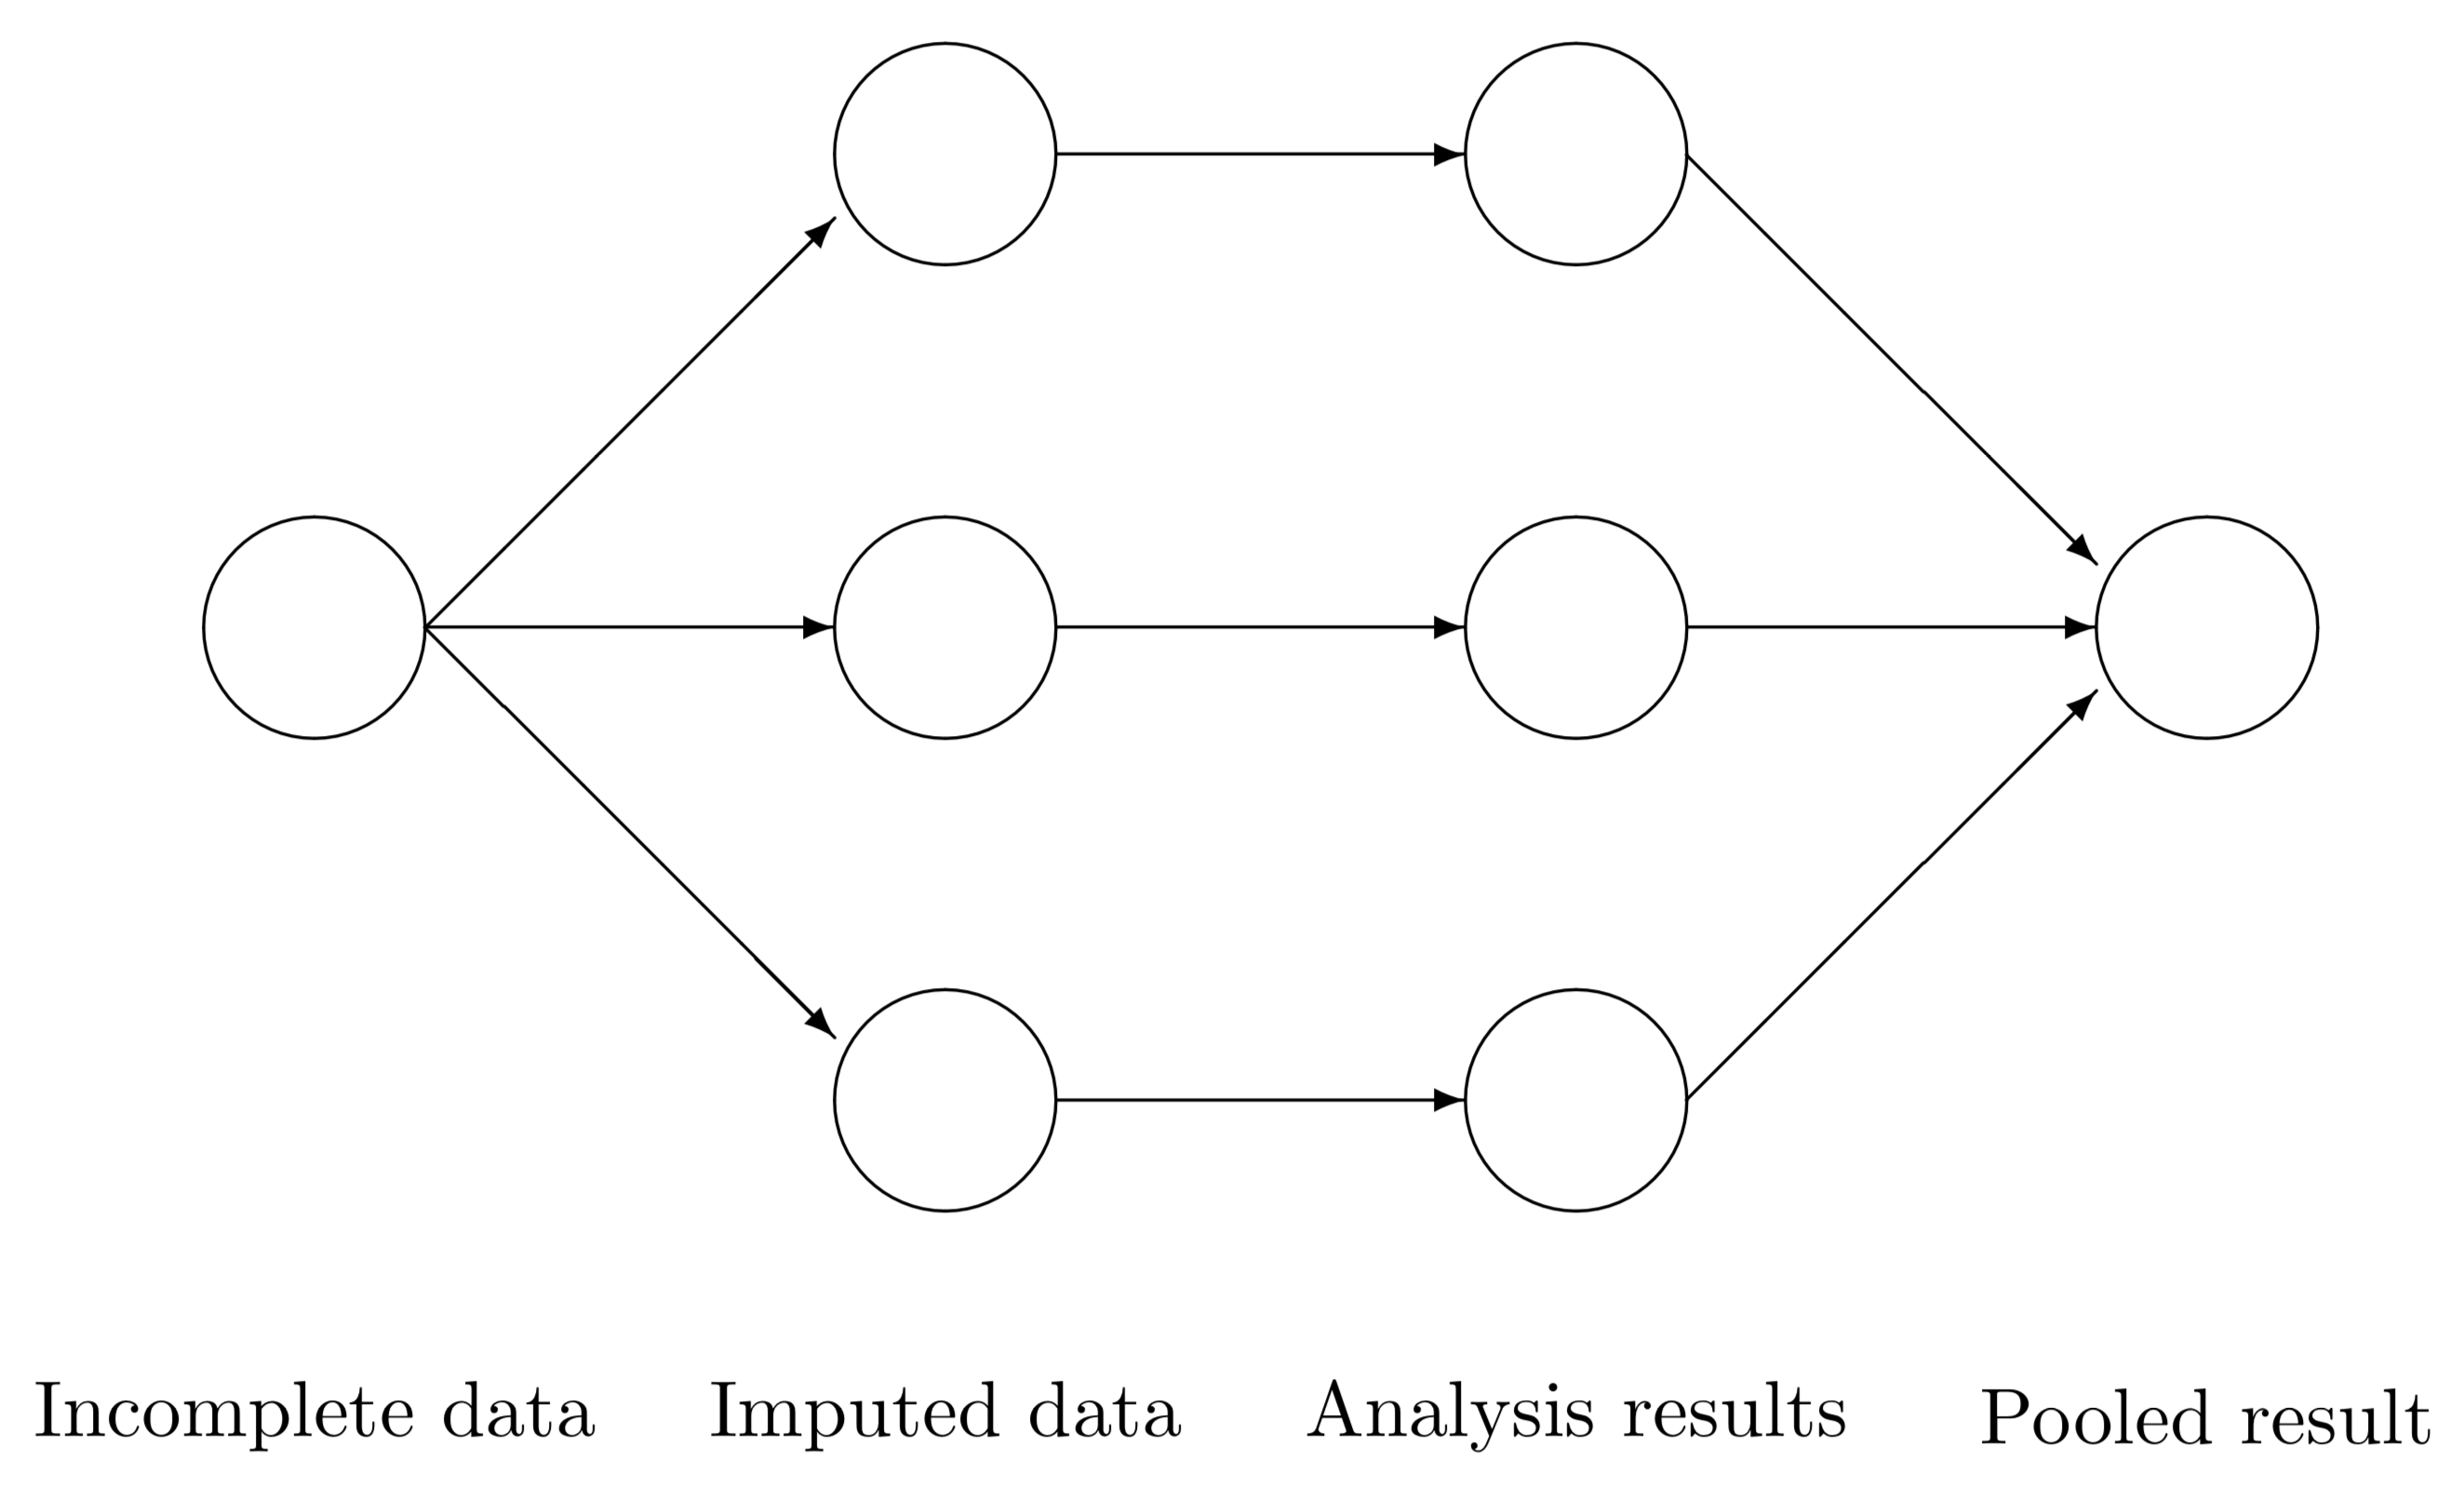
\includegraphics[scale=.2]{plots/miflow}
		\caption{Main steps used in \texttt{MICE} \citep{Buuren2011}}
		\label{fig6_1}
	\end{figure} 
	Figure \ref{fig6_1} illustrates how MICE solves a missing data problem by generating 3 imputed datasets. Three imputed datasets are generated with function \textbf{mice()}. Analysis are performed on every imputed dataset by \textbf{with()} function and combined into a single inference with function \textbf{pool()}. The software stores the output of each step in a particular class: \textbf{mids}, \textbf{mira} and \textbf{mipo}. More details about \texttt{MICE} package can be found in \citet{Buuren2011}.
	
	Two features of the software motivate our research. First, the default imputation method for numerical missing data is predictive mean matching (PMM) \citep{little1988missing}.
	\begin{lstlisting}
		library(mice, warn.conflicts = FALSE)
		imp <- mice(nhanes, print = FALSE)
		imp$method
	\end{lstlisting}
	\begin{verbatim}
		##   age   bmi   hyp   chl 
		##    "" "pmm" "pmm" "pmm"
	\end{verbatim}
	It generates imputations for a missing cell from its $p$ nearest points. The distance function applied to selection nearest points in MICE is:
	\begin{equation}
		\begin{array}{ll}
			d_{mice}(x_{i}^{obs}, x_{j}^{mis}) = |x_{i}^{obs}\beta^{*} - x_{j}^{mis}\hat{\beta}|,
		\end{array} 
	\end{equation}
	where $\hat{\beta}$ is the mean of the posterior distribution of models' parameters and $\beta^{*}$ is a random draw from the corresponding posterior distribution. Predictive mean matching is a non-parametric imputation approach that is proven to perform well in a wide range of scenarios \citep{de2011handbook, siddique2008multiple, su2011multiple, Buuren2018, Buuren2011, Vink2014, white2011multiple, Vink2015, yu2007evaluation}. The attractive advantage of PMM is that the imputed data is consistently within the range of the sample space \citep{heeringa2001multivariate, Buuren2018, Vink2014, Vink2015, white2011multiple, yu2007evaluation}. For instance, PMM prevents imputing negative values for data that are strictly non-negative. Second, \textbf{mids} only stores imputed datasets not the estimated parameters of the imputation models \citep{hoogland2020handling}. 
	
	Based on the features of \texttt{MICE} package discussed above, it is necessary to investigate whether PPC could check the donor selection procedure of PMM and perform PPC based on the observed data itself instead of the target statistics. \citet{he2012diagnosing} briefly discussed the approach to checking imputation models for subsets of missing variables. However, they assumed that the imputations of the remaining variables (excluding the incomplete variables of interest in an assessment) are adequate. Therefore, we also evaluate the performance of PPC when relaxing this assumption in the application section \ref{sec:6.6}.      
	
	The implement of PPC in \texttt{MICE} (version 3.13.15) is straightforward. A new argument \texttt{where} is included in \texttt{mice} function which allows us to replace the observed data by randomly drawing values from the predictive posterior distribution \citep{volker2021anonymiced}. Here is an example to generate replications of the observed data.   
	\begin{lstlisting}
		to_imp <- as.data.frame(!is.na(nhanes)) 
		imp <- mice(nhanes, where = to_imp, print = FALSE)
	\end{lstlisting}


	\section{Simulation Study}
	\label{sec:6.4}
	We carried out a simulation study to investigate the performance of the proposed diagnostic approach, varying several factors including missingness proportion (30\%, 50\%, 80\%), missingness mechanisms (MCAR and MARr), nominal levels of the confidence interval (75\%, 95\%) and different imputation models. The simulation study consisted of diagnostics under three scenarios: 1) quadratic equation with an incomplete outcome 2) quadratic equation with missing covariates 3) generalised linear model with an incomplete binary outcome. We evaluated whether the proposed diagnostic method could identify the congenial imputation model for continuous and discrete missing variables under the first and the third scenarios. We also investigated the performance of the proposed diagnostic method on the donor selection procedure of predictive mean matching under the second scenario. The sample size and the number of iterations were set to be 1000 and 50 separately in all simulations.  
	
	We induced missingness with the \texttt{ampute()} function in the simulation study. Generally, \texttt{ampute()} is a convenient function in \texttt{MICE} package to generate missing data for simulation purposes \citep{Schouten2018}. We considered missing completely at random (MCAR) mechanism where the probability of missingness is equal for every cell as well as right-tailed missing at random (MARr) mechanism where higher values of covariates have a higher probability of being unobserved. In the algorithm of \texttt{ampute()} function, the probability of missingness is allocated with different logistic functions of the weighted sum score, which is a linear combination of covariates correlated with the probability of missingness:
	\begin{equation}
		\begin{array}{ll}
			wss_{i} = w_{i}x_{1i} + w_{i}x_{2i} + \dots + w_{i}x_{mi}
		\end{array} 
	\end{equation}
	The weight $w_i$ is pre-specified to reflect the influence of the variable $x_{i}$ on the probability of missingness. For instance, if the formation of a weighted sum score is:
	$wss = x_1 + x_2$, the probability of missingness is determined by both $x_1$ and $x_2$ with the equal effects. More specifically, under MARr mechanism, candidates with higher values of weighted sum score have a higher probability of being unobserved when applying the \texttt{ampute()} function to generate missing data.
	
	\subsection{Quadratic equation with an incomplete outcome}
	In the first simulation study, we considered a partially observed variable $Y$ and a fully observed variable $X$. The data was generated from : $X \sim unif(-3, 3)$, $Y|X \sim \mathcal{N}(X + X^2, 1)$. The scientific model was indeed a quadratic model. We considered two imputation models for the missing response $Y$: one is a linear regression of $Y$ on $X$, and the other is a quadratic regression of $Y$ on $X$. 
	
	\subsection{Quadratic equation with incomplete covariates}
	In the second simulation study, the response variable $Y$ was generated from a normal distribution: $Y|X \sim \mathcal{N}(X + X^2, 1)$, where the covariate $X$ followed a standard normal distribution. In this simulation study, the response variable $Y$ was completely observed while the covariate $X$ and the corresponding quadratic term $X^2$ were jointly missing for a part of the cases. There were no cases with missing cells on either $X$ or $X^2$. We compared two non-parametric methods, predictive mean matching (PMM) and polynomial combination (PC) with a parametric method, the substantive model compatible fully conditional specification (SMC-FCS) \citep{Vink2013, bartlett2015multiple}. The PC and SMC-FCS methods are two accepted methods to impute linear regression with quadratic terms. The PC method is an extension of PMM but applies a different donor selection procedure. 
	
	\subsection{Generalised linear model for discrete variables}
	The final simulation study considered a partially observed binary $Y$ and two complete covariates $X$ and $Z$. The model of scientific interest was : $Pr (Y = 1 | X, Z) = exp(X + Z) / 1 + exp(X + Z)$,
	where $x \sim unif(-3 , 3)$ and $Z \sim \mathcal{N}(1, 1)$. Under MARr mechanism, the weights of variables $X$ and $Z$ in determining the probability of missingness for $Y$ were set to be equal. Since the logistic regression actually models the probability of assignment, we investigated the plot of deviance and calculated the sum of squared deviance divided by the sample size. There were two candidate models: a logistic regression of $Y$ on $X$ and $Z$ and a logistic regression of $Y$ on $Z$ only.
	
	\section{Simulation results}
	\label{sec:6.5}
	In this section, we present the simulation results of the proposed diagnostic method under three different scenarios. For numerical assessment, we estimated the rate by which the confidence interval covers the observed data (COV), the mean of the distance between the observed data and the mean of corresponding predictive posterior distributions (Distance), and the average width of the confidence intervals (CIW). We also provided graphical analyses with scatterplots, density plots, and distribution plots, which show observed values, upper and lower bounds of confidence intervals for each observed data point. Sometimes a single plot or summarised statistic is inadequate to arrive at a conclusion. Conducting PPC with various tools would provide a more comprehensive evaluation of the imputation model.     
	
	\subsection{Quadratic equation with an incomplete outcome}
	Table \ref{tab6_1} shows the results of the simulation study when the substantive model is a quadratic equation with an incomplete outcome. Since we only generated one incomplete dataset and repeated imputing it 50 times, all coverage rates were close to the pre-specified nominal level. However, when the imputation model was misspecified as a linear regression model, the average distance was larger than the average distance under the correct specification of the imputation model (linear regression with a quadratic term). It conforms to our intuitive idea that the data would be close to the centre of predictive posterior distributions if the model fits. The variance of the missing variable $Y$ was set as 1, which implied that the width of 95\% nominal confidence interval is approximate 3.92 ($1.96 \times 2$) and the width of 75\% nominal confidence interval is approximate 2.3 ($1.15 \times 2$). When the imputation model was correctly specified, the estimated average width of the confidence interval was unbiased. However, the variance of $Y$ was overestimated when the imputation model was linear. 
	
	The same result could also be derived from the graphical analysis. Figure \ref{fig6_2} shows distribution plots under the scenario of 30\% missing cases and MARr missing mechanism. This plot provides upper and lower bounds of the posterior predictive distribution for all observed $Y$ in ascending order of the mean of the posterior distribution. Green points imply the corresponding observed value falls in the interval, while red points imply the corresponding observed value falls out the interval. 
	
	When the imputation model was correctly specified, the points out of the 95\% confidence interval were randomly spread over the sample space without any patterns. However, when the imputation model was incorrectly specified as the linear regression model, the points out of the confidence interval clustered in the regions with extreme values of $X$. Moreover, the width of the intervals was generally narrower when the model was correct. The density plot and the scatter plot of the observed and replicated data generated with function \textbf{densityplot()} and \textbf{xyplot()} in \texttt{MICE} also show the evidence that the quadratic regression is preferable than the linear model (see figure \ref{fig6_3}). The scatter plot of the quadratic regression imputation model shows that replicated data overlapped the observed data. The density plot shows that the replicated data shared the same distribution as the observed data. This evidence illustrates the congeniality of the quadratic regression imputation model. However, the linear regression model performed worse than the quadratic regression model. First, the replicated data did not cover the observed data in two extreme regions in the scatter plot. Second, the empirical density of the replicated data and observed data were different. 
	
	These three plots do not merely illustrate the misspecification of the imputation model as the linear regression model. They also provide information to identify the regions of sample space in which the sub-optimal imputation model could still generate acceptable imputed values. Based on the distribution plot for the linear regression imputation model, we could also develop the piecewise linear regression model for the observed data. 
	
	When we cannot figure out the imputation model under which the observed data fit the predictive posterior distribution perfectly, these plots based on observed data provide the evidence of rebuilding a piecewise imputation model, which would improve the validity of imputation values. When the missing cases are not in the regions where outliers crowd, we could even apply the uncongenial imputation model. For example, in our simulation scenario, suppose we only consider the linear regression imputation model and missing cases with near parabolic minimum $X$ values. The imputed value will not show significant deviations from the true value. Finally, our proposed PPC approach for imputation models is robust against the different percentages of missing cases, missingness mechanisms, and the confidence interval's nominal levels. The nominal level of the confidence interval is determined by the extent to which we could undertake the outliers when the imputation model is not congenial with the data generating process. For instance, there were more outliers in the plot of means and 75\% confidence intervals than the plot of mean and 95\% confidence intervals. When we would like to replace the linear regression model with a piecewise linear model to improve the imputation, the selection knots based on the 75\% confidence intervals are more closed to the parabolic minimum than the 95\% confidence intervals (See figure \ref{fig6_4}). 
	
	\subsection{Quadratic equation with incomplete covariates}	
	Table \ref{tab6_2} and \ref{tab6_3} show the result of the simulation for the quadratic equation with incomplete covariates. Based on the numerical results, the performance of these three methods, PC, SMC-FCS, and PMM, was the same, despite the slightly reduced coverage rate of PMM. In fact, when the missingness mechanism is MCAR (to bypass the problem of the sparse observed region for PMM), PMM would also provide a valid inference of the regression parameters (see Table \ref{tab6_4}) \citep{Vink2013}.
	
	However, when it comes to graphical diagnostics, the misfit of PMM appears. The distribution plot (figure \ref{fig6_5} and \ref{fig6_6}) show that PC and SMC-FCS generated the same posterior predictive distribution of the observed data. There were more outliers with a larger value of $Y$. It is sensible since the density function of $X$ based on $Y$ is not monotone. Thus, it is unavoidable to impute the missing cell on the opposite arm of the parabolic function. Although in such a case, the imputed value was not the same as the true value, the replicated data still overlapped the observed data in the scatter plot (see Figures \ref{fig6_7}). The distribution plot of PMM with a 95\% nominal level in Figure \ref{fig6_5} did not show more outliers than these of PC and SMF-FCS. However, when the nominal level was set to 75\%, more outliers appeared in the sub-plot of PMM (Figure \ref{fig6_6}). The reason is that there are more observed data closed to the centre in the plots of PC and SMC-FCS, which implies the superiority of PC and SMC-FCS. The scatter plot also shows the discrepancy between the distribution of the replicated and the observed data with respect to PMM (Figures \ref{fig6_7}). The result is robust against various percentages of missing cases and over the studied missing mechanisms. The proposed PPC for the imputation model could check the donor selection process of hot-deck approaches. In our simulation scenarios, selecting donors for the composition $X + X^2$ performed better than only solving for the missing variable $X$. SMC-FCS was treated as the baseline in our simulation since it is proven as a reliable imputation method when the substantive model is known \citep{bartlett2015multiple}. The PC performs as well as the SMC-FCS which implies the donor selection process of PC reflects the data generating process in our simulation scenarios. However, when applying hot-deck approaches to implement imputation, the success in model checking is not sufficient to define valid imputations. In order to determine whether we could derive plausible imputations, additional diagnoses of distribution of the complete variable for observed and missing cases are necessary. For example, in our simulation scenario, if the variable $Y$'s range of missing cases is out of the range of observed cases, the PC may still derive implausible imputations. 
	
	\subsection{Generalised linear model for discrete variables}
	Table \ref{tab6_5} shows the average sum of squared deviance for two different logistic regression models. The value of the average sum of squared deviance was smaller when the imputation model was correctly specified with logistic regression on both $X$ and $Z$. The result is robust against the percentage of missing cases and missingness mechanisms. Figure \ref{fig6_8} shows that the residuals tend to zero when the imputation model fits the observed data better. The distribution of the observed data was more extreme than the empirical posterior distributions of replicated data generated under the logistic model with only variable $Z$. 
	
	\section{Application}
	\label{sec:6.6}
	\subsection{Background}
	We illustrate the application of the proposed PPC for multiple missing variables with the data from the body mass index (BMI) of the Dutch. This application is to study whether the proposed PPC works for a sequence of imputation models. More specifically, we aim to investigate whether the incorrect imputation model for one missing variable would disturb the proposed PPC for other variables. BMI is defined as the body weight divided by the square of the body height, which is broadly applied to categorise a person into underweight, normal, overweight, and obese. Since measuring a person's weight and height is costly, an alternative is to ask people to report their weight and height. However, such self-report data is systematically biased. People are used to overestimating their height and underestimating their weight, leading to a lower self-report BMI compared with measured BMI \citep[Section 9.3]{Buuren2018}. The goal of the study is to estimate unbiased BMI from the self-report data. We apply the multiple imputation approach to fill the unobserved measured weight and height. 
	
	The data we analyze is named \texttt{selfreport} in \texttt{MICE} package. The data consists of two components. One is the calibration dataset that contains 1257 Dutch individuals with both self-report and measured height and weight and was taken from \citet{krul2011self}. The original survey measured 4459 adults in either Italy, Netherlands, or North America aged 18-65 years in 1999 or 2000. The second part is the survey dataset containing 803 Dutch adults aged 18-75 years with only self-reported data. The survey data were collected in November 2007, either online or using paper-and-pencil methods \citep[Section 9.3]{Buuren2018}. Six variables are included in the application: \texttt{age} (years), \texttt{sex} (male or female), \texttt{hm} denoting measured height (cm), \texttt{hr} denoting self-reported height (cm), \texttt{wm} denoting measured weight (kg), and \texttt{wr} denoting self-reported weight (kg). 
	
	To fit the aim of this application study, we design two linear regression imputation models for \texttt{hm}: one includes all the other variables, and the other includes all the other variables except the variable \texttt{hr}. Similarly, there are two linear regression imputation models for \texttt{wm}: one includes all the other variables, and the other includes all the other variables except the variable \texttt{wr}. In such a case, we have four imputation strategies to evaluate:
	\begin{enumerate}
		\item Case 1: include \texttt{hr} in the imputation model of \texttt{hm} and \texttt{wr} in the imputation model of \texttt{wm}.
		\item Case 2: include \texttt{hr} in the imputation model of \texttt{hm} and exclude \texttt{wr} from the imputation model of \texttt{wm}.
		\item Case 3: exclude \texttt{hr} from the imputation model of \texttt{hm} and include \texttt{wr} in the imputation model of \texttt{wm}.
		\item Case 4: exclude \texttt{hr} from the imputation model of \texttt{hm} and \texttt{wr} from the imputation model of \texttt{wm}.
	\end{enumerate}
	Although it is evident that \texttt{hr} and \texttt{wr} are significant covariates for the imputation of \texttt{hm} and \texttt{wm}, we deliberately ignore these two variables in some cases to evaluate whether incorrect imputation model for \texttt{hm} (\texttt{wm}) influences PPC for \texttt{wm} (\texttt{hm}).
	 
	\subsection{Results}
	Table \ref{tab6_6} shows that the best imputation model among these four is the one that includes both \texttt{wr} and \texttt{hr}. The average distance and the width of confidence intervals for the observed data were the smallest for both \texttt{hm} and \texttt{wm}. No matter the imputation model of \texttt{hm} was correctly specified, the linear regression imputation model for \texttt{wm} should be based on all the other variables. When fixing the imputation model for the \texttt{hm} (no matter including \texttt{hr} or not), the average distance and the average width of the confidence interval of \texttt{hm} derived under the linear model included \texttt{hr} was remarkably less than the result taken under the linear model excluded the covariate \texttt{hr}. The graphical results (Figure \ref{fig6_9}-\ref{fig6_12}) show the same conclusion. When the linear regression imputation model for \texttt{wm} or \texttt{hm} was correctly specified, the imputed data overlapped the observed data in the scatter plot. The observed data would be closer to the centre of the confidence interval, and the width of confidence intervals was relatively small. However, the result of \texttt{wr} in case 3 was slightly larger than that in case 1. Similarly, the result of \texttt{wr} in case 4 was slightly larger than that in case 2. A similar result could be found in fixing the imputation model for the \texttt{wm} (no matter the imputation model includes \texttt{wr} or not). The average distance and the average confidence interval of \texttt{wm} derived under the linear model had \texttt{wr} was remarkably less than the result taken under the linear model excluded the covariate \texttt{wr}.
	
	The findings imply that incorrect specification of the imputation models for other missing variables $Y_{-j}$ would influence the target variable $Y_j$ for which we perform the PPC because densities of the imputed variables $Y_{-j}$ are different from the `true' densities. However, we can still select the correct model for $Y_j$. Our application scenario is relatively simple: the linear model is sufficient to reflect the data generating process of missing variables. However, we do not rule out the possibility that under extreme and complicated cases, incorrect specification of the imputation models for other missing variables $Y_{-j}$ would prevent us from selecting the most suitable imputation model for the missing variable $Y_j$. 
	
	\section{Discussion}
	\label{sec:6.7}
	The proposed imputation model diagnostic procedure based on PPC involves numerical assessment and graphical analysis. For numerical assessment, the evidence of a fitted imputation model is less deviation between the observed value and the expectation of corresponding predictive posterior distribution and narrower width of confidence intervals of predictive posterior distributions for the observed data. For graphical analysis, we provide the distribution plot, the scatter plot and the density plot. The more suitable imputation models are, the more similar the replicated data to the observed data in the density and scatter plots. The distribution plot shows posterior distributions of all observed data. It allows the researcher to identify the regions where the imputation model misfits. It is noteworthy that applying both numerical and graphical tools benefits a thorough understanding of model selection.
	
	The simulation study demonstrates that the proposed imputation model diagnostic procedure works on continuous and discrete variables under parametric and hot-deck multiple imputation approaches. We could derive more information for a continuous variable, such as the way to improve the imputation model, because of the distribution plot. For example, although the imputation model is incorrect in general, it provides valid imputations in the focused regions. In such a case, we could still apply the suboptimal imputation model. Moreover, we could only adjust the imputation model in the misfitted regions and develop a piecewise imputation model. The PPC for categorical data or ordered categorical data is limited, since the predictor of the imputation model is the probability of assignment rather than the observed data itself. We currently investigate residual deviance as the indicator to select the model for categorical data and ordered categorical data. For hot-deck imputation approaches, what PPC diagnoses is the donor-selection procedure. However, based on the features of predictive mean matching, the appropriate donor selection does not ensure plausible imputations. Extra analysis of the observed data and the imputed data is necessary.   
	
	The application example shows that the PPC works on the multivariate missing datasets. When the imputed covariate deviates from the actual distribution because of the mis-specified imputation models, the imputation model for the predictor could also be selected by PPC. In our case study, the misspecification of one missing variable slightly influences the other missing variable's numerical results. However, in more extreme situations, such as a large number of missing variables and more ridiculous imputation models for covariates, the result may be influenced seriously, so as to result in a sub-optimal model selection. Therefore, it is more reasonable to perform the numerical analysis of all missing variables and make the model selection for those variables with remarkably different results under different candidate imputation approaches first. 
	
	Existing PPC proposed by \citet{he2012diagnosing} and \citet{gelman2005multiple} measured the posterior predictive p-value to indicate the discrepancies of summarised statistics between the observed and replicated data. The close to 0 or 1 p-value implies the inadequacy of the imputation model with respect to the target quantities. The target quantities should be calculated with the completed data, which consists of the observed and the imputed data because it allows the researcher to calculate the target quantities requiring a complete data matrix. Both \citet{he2012diagnosing} and \citet{nguyen2015posterior} found that the existing PPC for multiple imputation model is sensitive to the percentage of missing cases. Since the imputed and replicated data are generated from the same posterior predictive distribution, the diagnostic becomes more difficult with an increasing proportion of missing data.
	
	Unlike the existing PPC approach, the PPC discussed in the paper checks the imputation model for each missing variable under the FCS framework. We diagnose the distribution of the observed data so that the result would also be reliable with a large proportion of missing cases. The simulation study also shows that the proposed PPC works for different missingness mechanisms. The PPC for multiple imputation models based on target analysis would be more informative when the imputer is also the researcher. The issue would be whether a valid inference for the scientific interest could be derived from the imputed data. However, the PPC for multiple imputation models based on the observed data addresses another issue: whether the imputation model is congenial to the substantive model. The imputed data generated after the proposed PPC could be used for more general downstream analysis and different scientific interests.
	
	When the sample size is tremendous, it is better to choose some representative data to check the imputation model so that the scatter plot or the distribution plot would not be too crowded. A clustered procedure could be applied to gather the observed data with closed values and choose one subset in each cluster to check the model. Further investigation is necessary to set the rule to select the observed data when the sample size is too large.
	
	\newpage
	\begin{sidewaystable}[ht!]
		\begin{tabular}{cc|cccc|cccc|cccc}
			\multicolumn{2}{l|}{}                             & \multicolumn{4}{c|}{COV}                                                                                           & \multicolumn{4}{c|}{Average Distance}                                                                              & \multicolumn{4}{c}{Average CIW}                                                                                   \\ \cline{3-14} 
			\multicolumn{1}{l}{}      & \multicolumn{1}{l|}{} & \multicolumn{2}{c}{linear model}                        & \multicolumn{2}{c|}{quadratic model}                     & \multicolumn{2}{c}{linear model}                        & \multicolumn{2}{c|}{quadratic model}                     & \multicolumn{2}{c}{linear model}                        & \multicolumn{2}{c}{quadratic model}                     \\ \hline
			\multicolumn{1}{l|}{}     & \multicolumn{1}{l|}{} & \multicolumn{1}{l}{75\%CI} & \multicolumn{1}{l}{95\%CI} & \multicolumn{1}{l}{75\%CI} & \multicolumn{1}{l|}{95\%CI} & \multicolumn{1}{l}{75\%CI} & \multicolumn{1}{l}{95\%CI} & \multicolumn{1}{l}{75\%CI} & \multicolumn{1}{l|}{95\%CI} & \multicolumn{1}{l}{75\%CI} & \multicolumn{1}{l}{95\%CI} & \multicolumn{1}{l}{75\%CI} & \multicolumn{1}{l}{95\%CI} \\
			\multicolumn{1}{c|}{}     & missingness           &                            &                            &                            &                             &                            &                            &                            &                             &                            &                            &                            &                            \\ \cline{2-14} 
			\multicolumn{1}{c|}{}     & 30                    & 0.76                       & 0.96                       & 0.75                       & 0.93                        & 2.41                       & 2.41                       & 0.79                       & 0.79                        & 6.64                       & 11.32                      & 2.27                       & 3.87                       \\
			\multicolumn{1}{c|}{MCAR} & 50                    & 0.72                       & 0.96                       & 0.76                       & 0.94                        & 2.44                       & 2.44                       & 0.77                       & 0.77                        & 6.61                       & 11.27                      & 2.25                       & 3.83                       \\
			\multicolumn{1}{c|}{}     & 80                    & 0.77                       & 0.95                       & 0.78                       & 0.94                        & 2.25                       & 2.25                       & 0.87                       & 0.87                        & 6.53                       & 11.13                      & 2.51                       & 4.28                       \\\hline
			\multicolumn{1}{c|}{}     & 30                    & 0.75                       & 0.95                       & 0.74                       & 0.94                        & 2.28                       & 2.28                       & 0.8                        & 0.8                         & 6.26                       & 10.66                      & 2.31                       & 3.94                       \\
			\multicolumn{1}{c|}{MARr} & 50                    & 0.76                       & 0.95                       & 0.73                       & 0.95                        & 2.21                       & 2.21                       & 0.81                       & 0.81                        & 6.3                        & 10.73                      & 2.3                        & 3.91                       \\
			\multicolumn{1}{c|}{}     & 80                    & 0.8                        & 0.96                       & 0.77                       & 0.92                        & 1.8                        & 1.8                        & 0.83                       & 0.83                        & 5.43                       & 9.25                       & 2.38                       & 4.05                      
		\end{tabular}
		\caption{The rate of nominal confidence interval covers the observed data (COV), the mean of the distance between the observed data and the location of the predictive posterior distribution (Distance), and the average width of the nominal (75\% and 95\%) confidence intervals (CIW) for two imputation models (linear model and quadratic model) under different combinations of experimental factors. The analysis model is a quadratic equation.}
		\label{tab6_1}
	\end{sidewaystable}
	
	\begin{sidewaystable}[ht!]
		\begin{tabular}{cc|ccc|ccc|ccc}
			\multicolumn{2}{l}{}                    & \multicolumn{3}{c|}{COV} & \multicolumn{3}{c|}{Average distance} & \multicolumn{3}{c}{Average CIW} \\ \cline{2-11} 
			\multicolumn{1}{c|}{}     & missingness & PC    & SMC-FCS  & PMM   & PC         & SMC-FCS      & PMM       & PC       & SMC-FCS    & PMM     \\
			\multicolumn{1}{c|}{}     & 30          & 0.94  & 0.94     & 0.91  & 0.62       & 0.62         & 0.68      & 3.02     & 3.1        & 3.03    \\
			\multicolumn{1}{c|}{MCAR} & 50          & 0.94  & 0.93     & 0.9   & 0.61       & 0.61         & 0.67      & 3.03     & 3.06       & 2.97    \\
			\multicolumn{1}{c|}{}     & 80          & 0.96  & 0.94     & 0.91  & 0.61       & 0.64         & 0.65      & 3.06     & 3.14       & 3       \\ \hline
			\multicolumn{1}{c|}{}     & 30          & 0.94  & 0.94     & 0.89  & 0.59       & 0.59         & 0.64      & 2.93     & 2.84       & 2.84    \\
			\multicolumn{1}{c|}{MARr} & 50          & 0.93  & 0.94     & 0.89  & 0.57       & 0.58         & 0.62      & 2.74     & 2.7        & 2.68    \\
			\multicolumn{1}{c|}{}     & 80          & 0.93  & 0.97     & 0.93  & 0.56       & 0.56         & 0.61      & 2.61     & 2.64       & 2.69   
		\end{tabular}
		\caption{The rate of nominal confidence interval covers the observed data (COV), the mean of the distance between the observed data and the location of the predictive posterior distribution (Distance), and the average width of the nominal 95\% confidence intervals (CIW) for PC, SMC-FCS and PMM under different combinations of experimental factors. The analysis model is a quadratic equation.}
		\label{tab6_2}
	\end{sidewaystable}
	
	\begin{sidewaystable}[ht!]
		\begin{tabular}{cc|ccc|ccc|ccc}
			\multicolumn{2}{l}{}                    & \multicolumn{3}{c|}{COV} & \multicolumn{3}{c|}{Average distance} & \multicolumn{3}{c}{Average CIW} \\ \cline{2-11} 
			\multicolumn{1}{c|}{}     & missingness & PC    & SMC-FCS  & PMM   & PC         & SMC-FCS      & PMM       & PC       & SMC-FCS    & PMM     \\
			\multicolumn{1}{c|}{}     & 30          & 0.76  & 0.75     & 0.7   & 0.62       & 0.62         & 0.68      & 1.77     & 1.82       & 1.78    \\
			\multicolumn{1}{c|}{MCAR} & 50          & 0.75  & 0.75     & 0.73  & 0.61       & 0.61         & 0.67      & 1.78     & 1.8        & 1.74    \\
			\multicolumn{1}{c|}{}     & 80          & 0.78  & 0.76     & 0.75  & 0.61       & 0.64         & 0.65      & 1.8      & 1.84       & 1.76    \\ \hline
			\multicolumn{1}{c|}{}     & 30          & 0.76  & 0.74     & 0.71  & 0.59       & 0.59         & 0.64      & 1.72     & 1.66       & 1.67    \\
			\multicolumn{1}{c|}{MARr} & 50          & 0.74  & 0.72     & 0.69  & 0.57       & 0.58         & 0.62      & 1.61     & 1.58       & 1.57    \\
			\multicolumn{1}{c|}{}     & 80          & 0.75  & 0.73     & 0.7   & 0.56       & 0.56         & 0.61      & 1.53     & 1.55       & 1.58   
		\end{tabular}
		\caption{The rate of nominal confidence interval covers the observed data (COV), the mean of the distance between the observed data and the location of the predictive posterior distribution (Distance), and the average width of the nominal 75\% confidence intervals (CIW) for PC, SMC-FCS and PMM under different combinations of experimental factors. The analysis model is a quadratic equation.}
		\label{tab6_3}
	\end{sidewaystable}
	
	\begin{table}[ht!]
		\begin{tabular}{cccc}
			& True value & Estimates value & Coverage rate \\
			$\beta_1$ & 1          & 1.008           & 0.934         \\
			$\beta_2$ & 1          & 1               & 0.958        
		\end{tabular}
		\caption{The PMM performs under the scientific model : $Y = \alpha + X\beta_{1} + X^2\beta_{2} +\epsilon$, where $\alpha = 0$, $\beta_{1} = 1$ and $\beta_{2} = 1$. The error term and variable $X$ follow standard normal distributions. 30\% cases of $X$ and $X^2$ are designed to be jointly missing. The missingness mechanism is MCAR.}
		\label{tab6_4}
	\end{table}
	
	\begin{table}[ht!]
		\begin{tabular}{cc|cc}
			&             & \multicolumn{2}{c}{mean of residual deviance} \\ \cline{2-4} 
			\multicolumn{1}{c|}{}     & missingness & with x               & without x               \\
			\multicolumn{1}{c|}{}     & 30          & 0.83                 & 1.25                    \\
			\multicolumn{1}{c|}{MCAR} & 50          & 0.85                 & 1.27                    \\
			\multicolumn{1}{c|}{}     & 80          & 0.95                 & 1.3                     \\ \hline
			\multicolumn{1}{c|}{}     & 30          & 0.9                  & 1.34                    \\
			\multicolumn{1}{c|}{MARr} & 50          & 0.94                 & 1.35                    \\
			\multicolumn{1}{c|}{}     & 80          & 0.98                 & 1.28                   
		\end{tabular}
		\caption{The average sum of squared deviance for two imputation models: 1) logistic regression with two predictors $x$ and $z$ 2) logistic regression with one predictor $x$ under different combinations of experimental factors. The outcome is a dichotomous variable $y$ and the binary regression is based on $x$ and $z$.}
		\label{tab6_5}
	\end{table}
	
	\begin{table}[ht!]
		\begin{tabular}{c|ccc|ccc}
			& \multicolumn{3}{c|}{hm}               & \multicolumn{3}{c}{wm}                \\ \cline{2-7} 
			& cov  & average distance & average CIW & cov  & average distance & average CIW \\
			strategy 1 & 0.95 & 1.57             & 8.27        & 0.95 & 2.28             & 12.46       \\
			strategy 2 & 0.95 & 1.65             & 8.89        & 0.94 & 10.9             & 54.38       \\
			strategy 3 & 0.95 & 5.58             & 26.89       & 0.94 & 2.35             & 12.83       \\
			strategy 4 & 0.95 & 5.56             & 27.88       & 0.97 & 9.84             & 59.57      
		\end{tabular}
		\caption{The performance of 4 imputation strategies is summarised by the coverage rate, the average distance and the average width of confidence intervals with respect to missing variables \texttt{hm} and \texttt{wm}}
		\label{tab6_6}
	\end{table}
	
	\newpage
	\begin{figure}[b]
		\begin{center}
			\resizebox{\textwidth}{!}{
				\subfigure[quadratic imputation model]{
					\label{boxplot:a}
					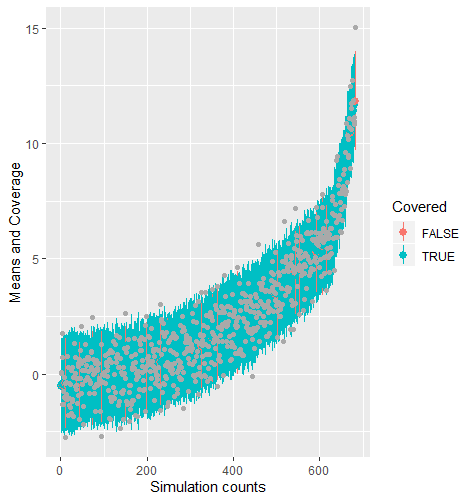
\includegraphics[scale=.5]{plots/plot6.1}
				}
				\subfigure[linear imputation model]{
					\label{boxplot:b}
					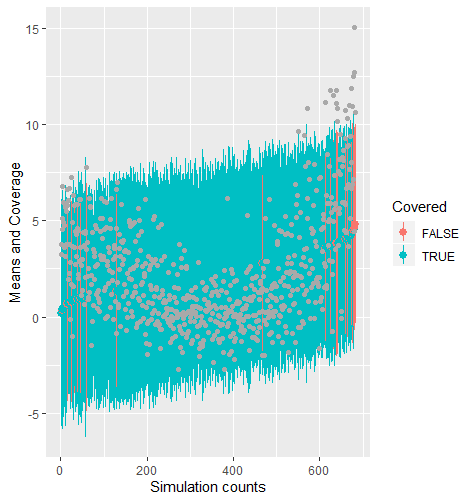
\includegraphics[scale=.5]{plots/plot6.2}
				}
			}
		\end{center}
		\caption{Distribution plots for the first simulation study (quadratic equation with an incomplete outcome) generated under 30\% missing cases and MARr missingness mechanism. The confidence interval is 95\% nominal.}
		\label{fig6_2}
	\end{figure}
	
	\begin{figure}[ht!]
		\begin{center}
			\resizebox{\textwidth}{!}{
				\subfigure[quadratic imputation model]{
					\label{boxplot:a}
					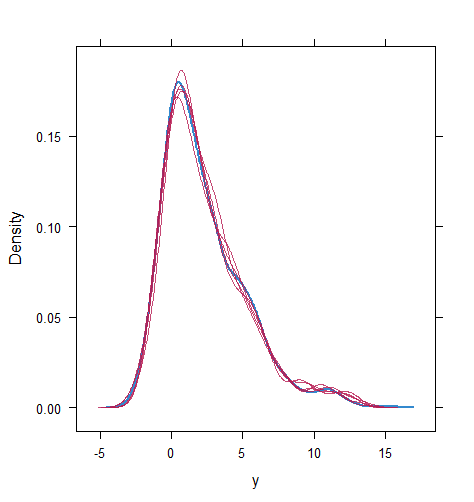
\includegraphics[scale=.5]{plots/plot6.3}
				}
				\subfigure[linear imputation model]{
					\label{boxplot:b}
					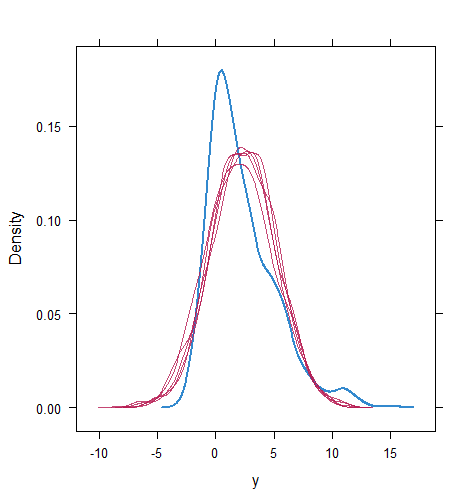
\includegraphics[scale=.5]{plots/plot6.4}
				}
			}\\ 	
			\resizebox{\textwidth}{!}{
				\subfigure[quadratic imputation model]{
					\label{boxplot:c}
					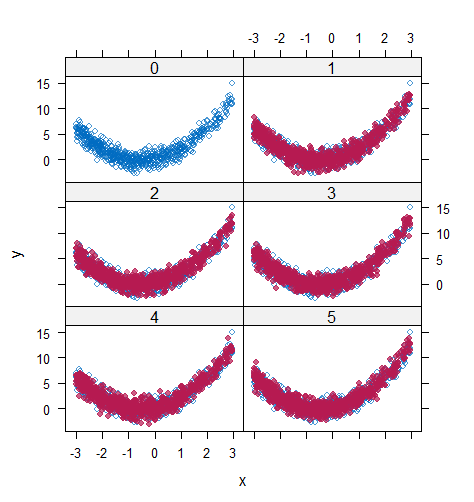
\includegraphics[scale=.5]{plots/plot6.5}
				}
				\subfigure[linear imputation model]{
					\label{boxplot:d}
					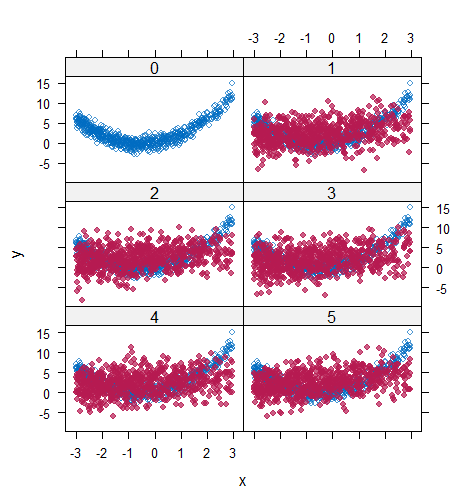
\includegraphics[scale=.5]{plots/plot6.6}
				}
			}
		\end{center}
		\caption{Scatterplots and densityplots for the first simulation study (quadratic equation with an incomplete outcome) generated under 30\% missing cases and MARr missingness mechanism.}
		\label{fig6_3}
	\end{figure}
	
	\begin{figure}[ht!]
		\begin{center}
			\resizebox{\textwidth}{!}{
				\subfigure[quadratic imputation model]{
					\label{boxplot:a}
					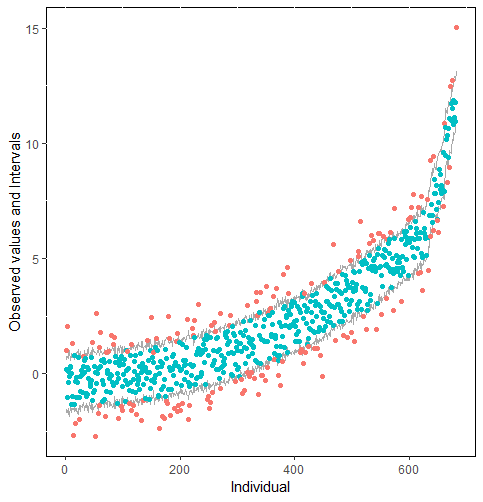
\includegraphics[scale=.5]{plots/plot6.7}
				}
				\subfigure[linear imputation model]{
					\label{boxplot:b}
					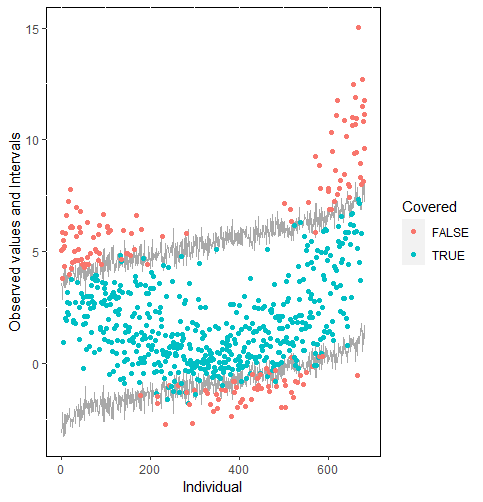
\includegraphics[scale=.5]{plots/plot6.8}
				}
			}
		\end{center}
		\caption{Distribution plots for the first simulation study (quadratic equation with an incomplete outcome) generated under 30\% missing cases and MARr missingness mechanism. The confidence interval is 75\% nominal.}
		\label{fig6_4}
	\end{figure}
	
		\begin{sidewaysfigure}
		\begin{center}
			\resizebox{\textwidth}{!}{
				\subfigure[PC]{
					\label{boxplot:a}
					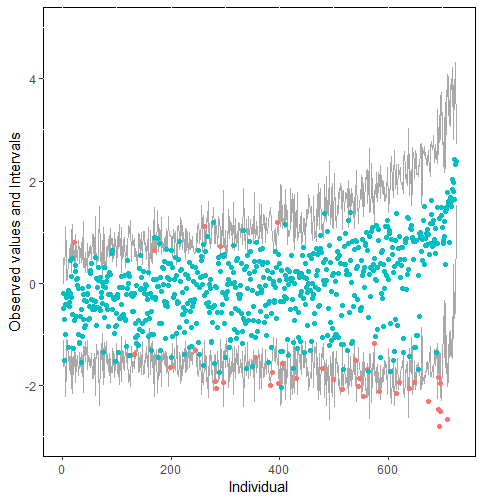
\includegraphics[scale=.5]{plots/plot6.9}
				}
				\subfigure[SMC-FCS]{
					\label{boxplot:b}
					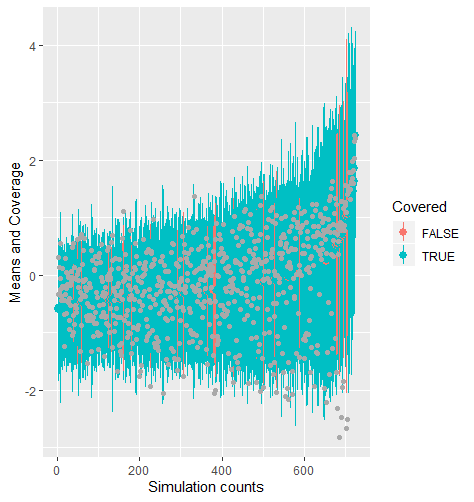
\includegraphics[scale=.5]{plots/plot6.10}
				}
				\subfigure[PMM]{
					\label{boxplot:b}
					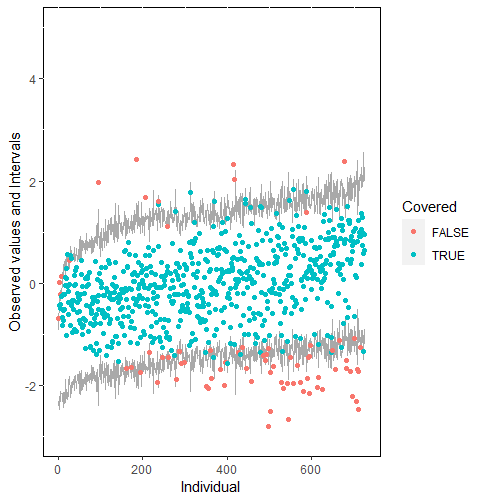
\includegraphics[scale=.5]{plots/plot6.11}
				}
			}
		\end{center}
		\caption{Distribution plots for the second simulation study (quadratic equation with incomplete covariates) generated under 30\% missing cases and MARr missingness mechanism. The nominal level is 95\%.}
		\label{fig6_5}
			\end{sidewaysfigure}
		
			\begin{sidewaysfigure}[ht!]
			\begin{center}
				\resizebox{\textwidth}{!}{
					\subfigure[PC]{
						\label{boxplot:a}
						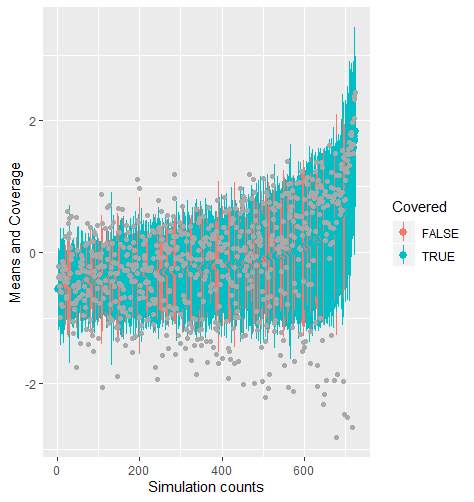
\includegraphics[scale=.5]{plots/plot6.12}
					}
					\subfigure[SMC-FCS]{
						\label{boxplot:b}
						\includegraphics[scale=.5]{plots/plot6.13}
					}
					\subfigure[PMM]{
						\label{boxplot:b}
						\includegraphics[scale=.5]{plots/plot6.14}
					}
				}
			\end{center}
			\caption{Distribution plots for the second simulation study (quadratic equation with incomplete covariates) generated under 30\% missing cases and MARr missingness mechanism. The nominal level is 75\%.}
			\label{fig6_6}
	
	\end{sidewaysfigure}
	
	\begin{sidewaysfigure}[ht!]
		\begin{center}
			\resizebox{\textwidth}{!}{
				\subfigure[PC]{
					\label{boxplot:a}
					\includegraphics[scale=.5]{plots/plot6.15}
				}
				\subfigure[SMC-FCS]{
					\label{boxplot:b}
					\includegraphics[scale=.5]{plots/plot6.16}
				}
				\subfigure[PMM]{
					\label{boxplot:b}
					\includegraphics[scale=.5]{plots/plot6.17}
				}
			}
		\end{center}
		\caption{Scatterplots for the second simulation study (quadratic equation with incomplete covariates) generated under 30\% missing cases and MARr missingness mechanism.}
		\label{fig6_7}
	\end{sidewaysfigure}

	\begin{figure}[ht!]
		\begin{center}
			\resizebox{\textwidth}{!}{
				\subfigure[logistic model based on $X$ and $Z$]{
					\label{boxplot:a}
					\includegraphics[scale=.5]{plots/plot6.18}
				}
				\subfigure[logistic model based on $Z$]{
					\label{boxplot:b}
					\includegraphics[scale=.5]{plots/plot6.19}
				}
			}
		\end{center}
		\caption{The plot of deviance residuals for the third simulation study (generalized linear model for discrete variables) generated under two logistic regression imputation models. The percentage of missing is 30\%, and the missingness mechanism is MARr.}
		\label{fig6_8}
	\end{figure}
	
	
	
	\begin{figure} [ht!]
		\centering
		\begin{tabular}{cccc}
			\includegraphics[width=0.3\textwidth]{plots/densitycase1} &
			\includegraphics[width=0.3\textwidth]{plots/scattercase1hm} &
			\includegraphics[width=0.3\textwidth]{plots/scattercase1wm} \\
			\textnormal{(a)}  & \textnormal{(b)} & \textnormal{(c)}  \\[6pt]
		\end{tabular}
		\begin{tabular}{cccc}
			\includegraphics[width=0.3\textwidth]{plots/distributioncase1hm} &
			\includegraphics[width=0.3\textwidth]{plots/distributioncase1wm} \\
			\textnormal{(d)}  & \textnormal{(e)}  \\[6pt]
		\end{tabular}
		\caption{Graphical analysis of the BMI data with imputation strategy case 1. (a) density plots, (b) scatter plot of \texttt{hm}, (c) scatter plot of \texttt{wm}, (d) distribution plot of \texttt{hm} and (e) distribution plot of \texttt{wm}.}
		\label{fig6_9}
	\end{figure}
	
	
	\begin{figure} [ht!]
		\centering
		\begin{tabular}{cccc}
			\includegraphics[width=0.3\textwidth]{plots/densitycase2} &
			\includegraphics[width=0.3\textwidth]{plots/scattercase2hm} &
			\includegraphics[width=0.3\textwidth]{plots/scattercase2wm} \\
			\textnormal{(a)}  & \textnormal{(b)} & \textnormal{(c)}  \\[6pt]
		\end{tabular}
		\begin{tabular}{cccc}
			\includegraphics[width=0.3\textwidth]{plots/distributioncase2hm} &
			\includegraphics[width=0.3\textwidth]{plots/distributioncase2wm} \\
			\textnormal{(d)}  & \textnormal{(e)}  \\[6pt]
		\end{tabular}
		\caption{Graphical analysis of the BMI data with imputation strategy case 2. (a) density plots, (b) scatter plot of \texttt{hm}, (c) scatter plot of \texttt{wm}, (d) distribution plot of \texttt{hm} and (e) distribution plot of \texttt{wm}.}
		\label{fig6_10}
	\end{figure}
	
	\begin{figure} [ht!]
		\centering
		\begin{tabular}{cccc}
			\includegraphics[width=0.3\textwidth]{plots/densitycase3} &
			\includegraphics[width=0.3\textwidth]{plots/scattercase3hm} &
			\includegraphics[width=0.3\textwidth]{plots/scattercase3wm} \\
			\textnormal{(a)}  & \textnormal{(b)} & \textnormal{(c)}  \\[6pt]
		\end{tabular}
		\begin{tabular}{cccc}
			\includegraphics[width=0.3\textwidth]{plots/distributioncase3hm} &
			\includegraphics[width=0.3\textwidth]{plots/distributioncase3wm} \\
			\textnormal{(d)}  & \textnormal{(e)}  \\[6pt]
		\end{tabular}
		\caption{Graphical analysis of the BMI data with imputation strategy case 3. (a) density plots, (b) scatter plot of \texttt{hm}, (c) scatter plot of \texttt{wm}, (d) distribution plot of \texttt{hm} and (e) distribution plot of \texttt{wm}.}
		\label{fig6_11}
	\end{figure}
	
	
	\begin{figure} [ht!]
		\centering
		\begin{tabular}{cccc}
			\includegraphics[width=0.3\textwidth]{plots/densitycase4} &
			\includegraphics[width=0.3\textwidth]{plots/scattercase4hm} &
			\includegraphics[width=0.3\textwidth]{plots/scattercase4wm} \\
			\textnormal{(a)}  & \textnormal{(b)} & \textnormal{(c)}  \\[6pt]
		\end{tabular}
		\begin{tabular}{cccc}
			\includegraphics[width=0.3\textwidth]{plots/distributioncase4hm} &
			\includegraphics[width=0.3\textwidth]{plots/distributioncase4wm} \\
			\textnormal{(d)}  & \textnormal{(e)}  \\[6pt]
		\end{tabular}
		\caption{Graphical analysis of the BMI data with imputation strategy case 4. (a) density plots, (b) scatter plot of \texttt{hm}, (c) scatter plot of \texttt{wm}, (d) distribution plot of \texttt{hm} and (e) distribution plot of \texttt{wm}.}
		\label{fig6_12}
	\end{figure}
	
	
	
	

		%\appendix
		%\include{appendix}
		
		\backmatter%%%%%%%%%%%%%%%%%%%%%%%%%%%%%%%%%%%%%%%%%%%%%%%%%%%%%%%
		\bibliographystyle{apalike-url}
		\bibliography{dissertation}
		\addcontentsline{toc}{chapter}{List of Figures}
\listoffigures

		\addcontentsline{toc}{chapter}{List of Tables}
\listoftables %	
		\chapter*{Samenvatting}
\addcontentsline{toc}{chapter}{Summary in Dutch / Samenvatting}
\markboth{Samenvatting}{Samenvatting}


Joint modeling (JM) en fully conditional specification (FCS) zijn twee veelgebruikte strategieën om multivariate incomplete data te imputeren. JM bestaat uit het specificeren van een multivariate verdeling voor de ontbrekende data om vervolgens imputaties uit de betreffende conditionele verdelingen te trekken. Bij FCS specificeert men de verdeling van iedere gedeeltelijk geobserveerde variabele conditioneel op alle andere variabelen. FCS heeft als voordeel boven JM dat het modeleren van multivariate data zeer flexibel kan worden vormgegeven. Het komt echter in de praktijk met regelmaat voor dat bepaalde structuren in de ontbrekende gegevens niet adequaat gemodelleerd kunnen worden. Daarnaast is het vaak lastig om de relaties tussen meerdere variabelen te bewaren wanneer een stapsgewijze imputatietechniek als FCS wordt gebruikt. Deze dissertatie heeft als doel om hybride imputatiestrategieën te ontwikkelen waarin aantrekkelijke eigenschappen van JM en FCS worden samengenomen. In dit proefschrift draag ik oplossingen aan voor ontbrekende dataproblemen waarin het toepassen van enkel JM of FCS tot suboptimale oplossingen leidt. 

In Hoofdstuk 2 beschouw ik algemene methoden om gekwadarateerde relaties te imputeren. Ik verbeter de polynomial combination (PC) methode en evalueer deze verbetering tegen oplossingen verkregen middels het Substantive Model Compatible Fully Conditional Specification (SMCFCS) framework. De uitkomst van deze evaluatie is als volgt: Als de ware verdeling en model bekend zijn, dan levert SMCFCS de scherpste inferentie. Dit gaat wel ten koste van de flexibiliteit in modelleren. Met de aangepaste PC methode blijft deze flexibiliteit wél behouden, maar kan de inferentie wat minder scherp zijn in situaties waar de verdeling van de geobserveerde data soms spaars is.

In Hoofdstuk 3 ontwikkel ik Multivariate Predictive Mean Matching (MPMM). Met MPMM kan men meer dan één incomplete variabele tegelijk imputeren. Ik combineer de methodologie van univariate PMM (REF LITTLE REF RUBIN) en canonical regression analysis (REF) om de ruimtes van de voorspellers en uitkomsten samen te vatten. Het voordeel van deze imputatiemethode is dat de relaties tussen incomplete variabelen behouden kunnen worden. Ik behandel een aantal scenario’s waarin MPMM gebruikt kan worden en beschouw de beperkingen van deze nieuwe methode. 

In Hoofdstuk 4 ontwikkel ik een hybride imputatietechniek om individuele behandeleffecten te kunnen schatten. Het imputeren van niet-geobserveerde uitkomsten maakt het mogelijk om verschillen tussen potentiele uitkomsten te berekenen voor verschillende behandelcondities. Het fundamentele probleem hierbij is dat beide uitkomsten nooit tegelijk geobserveerd kunnen worden. Men moet dus aannames doen over de correlatie tussen de potentiele uitkomsten. De voorgestelde hybride imputatiemethode stelt ons in staat om de partiële correlatie te specificeren en een sensitiviteitsanalyse uit te voeren. Ik demonstreer de validiteit van de voorgestelde hybride imputatiemethode en laat zien hoe men deze techniek in de praktijk kan toepassen. 
 
In Hoofdstuk 5 onderzoek ik de compatibiliteit van FCS onder informatieve prior verdelingen. Dergelijke vergelijkingen zijn al door meerdere auteurs beschreven voor scenarios waarin de prior voor de conditionele modellen niet informatief is. Compatibiliteit eigenschappen voor informatieve priors zijn echter onderbelicht gebleven. Ik toon aan dat FCS onder het normale lineaire model met een informatieve inverse-gamma prior compatibel is met een gezamenlijke verdeling en lever de bijbehorende normale inverse-Wishart prior verdeling voor de gezamenlijke verdeling.  

In Hoofdstuk 6 ontwikkel ik een nieuwe strategie voor het diagnosticeren en evalueren van multiple imputation modellen door middel van posterior predictive checking. Het idee hierbij is dat, wanneer het imputatiemodel congenial (REF MENG) is met betrekking tot het inhoudelijke analysemodel, de verwachte waarde van de geobserveerde data zich in het midden van de bijbehorende posterior predictive verdeling bevindt. Door de voorgestelde diagnostische methode te gebruiken, kunnen onderzoekers de geobserveerde data vergelijken met de ‘overgeïmputeerde’ data om de fit van het imputatiemodel te evalueren. 
 

		%%%%%%%%%%%%%%%%%%%%%%%%%%%%%%%%%%%%%%%%%%%%%%%%%%%%%%%%%%%%%%%%%%%%%%
		
		%for cosmetic reasons I include the back cover
		% REMOVE THE BELOW LINE WHEN SENDING TO PRINTER
		%\includepdf{cover_back.pdf}
		
	\end{document}
